% !TEX program = pdflatex
\documentclass[11pt]{article}
\usepackage[margin=0.82in]{geometry}
\usepackage[T1]{fontenc}
\usepackage[utf8]{inputenc}
\usepackage{newtxtext,newtxmath}
\usepackage{amsmath}
\usepackage{booktabs,longtable,array,calc}
\usepackage{graphicx}
\usepackage{xcolor}
\usepackage{microtype}
\usepackage{setspace}
\usepackage{caption}
\usepackage{float}
\usepackage{etoolbox}
\usepackage[round,authoryear]{natbib}
\usepackage[colorlinks=true,linkcolor=blue,citecolor=blue,urlcolor=blue,breaklinks=true]{hyperref}
\usepackage{bookmark}
\usepackage{xurl}
\usepackage{titlesec}
\usepackage{fancyhdr}
\usepackage{footnotehyper}
\makesavenoteenv{longtable}
\usepackage{ragged2e}

\singlespacing
\setlength{\parindent}{1.2em}
\setlength{\parskip}{0.18em}
\setlength{\emergencystretch}{3em}
\setcounter{secnumdepth}{2}
\setcounter{tocdepth}{2}
\titleformat{\section}{\large\bfseries}{\thesection.}{0.5em}{}
\titleformat{\subsection}{\normalsize\bfseries}{\thesubsection}{0.5em}{}
\titlespacing*{\section}{0pt}{1.0em}{0.45em}
\titlespacing*{\subsection}{0pt}{0.75em}{0.3em}
\captionsetup{font=small,labelfont=bf,justification=centering}
\pagestyle{fancy}
\fancyhf{}
\fancyfoot[C]{\thepage}
\renewcommand{\headrulewidth}{0pt}
\urlstyle{same}
\providecommand{\tightlist}{\setlength{\itemsep}{0pt}\setlength{\parskip}{0pt}}
\newcommand{\real}[1]{#1}
\AtBeginEnvironment{longtable}{\setlength{\tabcolsep}{3.5pt}}
\begin{document}
\justifying

\begin{center}
{\LARGE\bfseries News-Based Exchange-Rate Risk, Market Alignment, and Volatility Dynamics across African Economies\par}
\vspace{0.35em}
{\large\itshape Continental Panels, GARCH-Family Heterogeneity, Dynamic Transmission, and Out-of-Sample Forecast Evidence\par}
\end{center}
\vspace{0.6em}

\begin{abstract}
We introduce a market-alignment framework for organizing cross-country heterogeneity in news-based exchange-rate risk transmission and separate three empirical objects that are often conflated: information content, conditional-variance transmission, and forecast value. Using a 51-country African panel drawn from 54 source markets over January 2015--December 2025, we show that the News-Based Exchange-Rate Risk Index (NBERI) carries leading information about subsequent FX volatility, that transmission is materially stronger in markets where the FX-risk narrative is closely aligned with the bilateral exchange-rate level, and that the conditional-variance channel is selective rather than universal. In the continental benchmark, lagged NBERI predicts next-month volatility after controlling for volatility history, returns, inflation, country effects, and common time shocks ($\beta=0.030$, $p=0.004$), and remains significant after shared currencies are collapsed to 36 market clusters. Full-panel interaction tests imply an aligned-group slope of 0.063 ($p=0.007$) versus 0.017 ($p=0.147$) elsewhere, while a 1,000-draw random-subset benchmark places the selected group's effect near the upper tail of comparably sized groups. In the 15 aligned markets, the horizon-1 local-projection response is 0.121 ($p<0.001$), NBERI explains 3.39 percent of 12-month volatility forecast-error variance, and adding NBERI improves 2023--2025 pooled RMSE by 0.89 percent. Profile-likelihood GARCH-family tests with false-discovery-rate control identify robust conditional-variance effects only in Ghana and Libya. The evidence therefore distinguishes broad leading information from selective variance transmission and modest but genuine forecast value.
\end{abstract}

\noindent\textbf{Keywords:} news-based risk; exchange rates; volatility; market alignment; GARCH-X; local projections; Africa\\
\noindent\textbf{JEL Classification:} F31, C22, C23, C53, G15
\vspace{0.5em}
\section{Introduction}\label{introduction}

Exchange-rate instability remains a recurrent source of macroeconomic
risk across African economies. Depreciation passes into import prices,
changes the domestic-currency value of external liabilities, complicates
monetary policy, and can intensify balance-sheet and liquidity
pressures. Yet many conventional surveillance indicators are observed
only after these pressures have appeared in exchange rates, reserves,
inflation, or external financing conditions. A risk measure that
consistently moves before observed currency stress can therefore be
useful even if it does not replace market-based volatility models.

News-based indicators provide one route to earlier measurement. Economic
reporting aggregates dispersed information about foreign-exchange
availability, reserve adequacy, external financing, policy adjustments,
debt negotiations, devaluation expectations, and market access. The
broader uncertainty literature shows that disciplined text-based indices
can contain macroeconomic information that is not reducible to
contemporaneous market movements \citep{baker2016,caldara2022}. In foreign-exchange markets, the economic content
of news is especially plausible because prices respond rapidly to
changes in the information set \citep{andersen2003}. The empirical
question is whether a focused exchange-rate risk index adds information
after the currency market\textquotesingle s own history and
macroeconomic controls are taken into account.

This paper studies the News-Based Exchange-Rate Risk Index (NBERI), a
monthly measure of foreign-exchange and external-sector risk narratives.
The index is treated strictly as an information-state variable: it is
not market volatility, not an exchange-rate transformation, and not a
mechanical restatement of realized depreciation.\footnote{This distinction is substantive rather than semantic: NBERI is constructed from news narratives, whereas every market outcome in the paper is constructed from observed bilateral exchange-rate data.} The empirical question
is whether the information environment summarized by NBERI precedes
subsequent exchange-rate instability after the market\textquotesingle s
own history and conventional macroeconomic controls are taken into
account.

The paper\textquotesingle s central contribution is a market-alignment
framework for organizing cross-country heterogeneity in news-based
FX-risk transmission. Rather than treating country differences as a
collection of post hoc stories, the framework ranks eligible markets by
the contemporaneous alignment between the FX-risk narrative and the
bilateral exchange-rate level and then tests whether alignment predicts
stronger subsequent risk-to-volatility transmission in the full panel.
The selected 15-market group is also benchmarked against 1,000 random
15-country subsets. The ranking is descriptive rather than causal; its
contribution is to provide a disciplined organizing device for
heterogeneity that can be validated outside the selected subsample.\footnote{Market alignment is therefore not used as an instrument, treatment, or structural parameter. The full-panel interactions and random-subset benchmark are the formal tests of whether the aligned group exhibits unusually strong transmission.}

The second contribution is to separate three empirical objects that are
often conflated: information content, conditional-variance transmission,
and forecast value. Two-way fixed effects, PVARs, and local projections
ask whether NBERI contains leading information about future instability;
GARCH-X, EGARCH-X, and GJR/TGARCH-X ask whether NBERI enters the
conditional-variance recursion after endogenous volatility persistence
is absorbed; and expanding-window forecasts ask whether the signal
improves genuine out-of-sample loss. The paper does not require these
objects to agree. Their divergence is itself informative about how
news-based FX risk enters currency markets.\footnote{A variable can forecast future realized volatility without entering a particular parametric conditional-variance recursion, and an in-sample predictive relation can exist without producing economically large out-of-sample forecast gains.}

The continental design provides the empirical support needed to make
those contributions credible. The source panel contains 54 countries, of
which 51 satisfy pre-model coverage and return-variation criteria, while
a 36-market currency-cluster robustness design prevents repeated CFA- or
Common-Monetary-Area exchange-rate paths from being counted as
independent evidence.\footnote{This adjustment is especially important for the WAEMU/CEMAC CFA zones and tightly linked Common Monetary Area currencies, where repeated country labels can otherwise overstate the effective cross-section.} This broad benchmark establishes the common
leading-information result before the analysis turns to aligned-market
heterogeneity.

The results support that framework. The continental coefficient is 0.030
(p = 0.004), while the aligned-group full-panel slope is 0.063 (p =
0.007) and the remaining-market slope is 0.017 (p = 0.147). The
horizon-1 local-projection effect is also significantly larger for the
aligned group (increment = 0.072, p = 0.019), and the selected
group\textquotesingle s fixed-effects effect lies around the 94th
percentile of 1,000 random 15-country subsets. Yet conditional-variance
evidence is selective: after profile-likelihood refinement and
within-family false-discovery-rate correction, robust NBERI variance
effects survive only for Ghana under EGARCH-X and Libya under GARCH-X.
Out-of-sample gains are positive but modest. The paper therefore
contributes a unified empirical distinction between broad news-based
information, alignment-dependent transmission, and genuinely
market-specific variance effects.

\section{Related Literature and Testable Hypotheses}\label{related-literature-and-testable-hypotheses}

\subsection{News, information, and exchange-rate
risk}\label{news-information-and-exchange-rate-risk}

Newspaper-based uncertainty measures occupy an empirical space between
realized market variables and survey expectations. \citet{baker2016} establish that a transparent newspaper-coding framework can
generate an uncertainty index with macroeconomic content, while \citet{caldara2022} show that a focused text-based index can isolate a
particular class of risk. These contributions do not imply that media
coverage mechanically causes asset-price volatility. Their relevance is
informational: news can aggregate policy signals, funding conditions,
geopolitical developments, and expectations before those forces are
fully reflected in observed outcomes.

Foreign-exchange markets provide a demanding setting for such a test.
\citet{andersen2003} document rapid exchange-rate responses to
macroeconomic information, emphasizing that the surprise component of
news matters for price discovery. Across African economies, information
transmission is further shaped by heterogeneous exchange-rate regimes,
market depth, intervention practices, foreign-exchange availability, and
the presence of currency unions. A useful empirical design must
therefore allow both a common continental signal and substantial
cross-market heterogeneity rather than assigning a separate narrative to
every country coefficient.

\subsection{Conditional volatility and panel
dependence}\label{conditional-volatility-and-panel-dependence}

ARCH and GARCH models remain the standard parametric framework for
persistent conditional heteroskedasticity \citep{engle1982,bollerslev1986}. EGARCH permits asymmetric responses in log variance \citep{nelson1991}, while GJR-GARCH allows negative and positive innovations to
affect conditional variance differently \citep{glosten1993}. GARCH-X extensions provide a direct test of whether an
observed state variable contributes to conditional variance after
endogenous volatility persistence is absorbed \citep{francq2019,pedersen2019}. In the present setting, that distinction is
critical: a news-risk measure can predict next-month instability without
necessarily entering every currency\textquotesingle s variance recursion
through the same parameter.

Panel settings add a second complication: contemporaneous shocks and
common institutions generate cross-sectional dependence. \citet{cermeno2006} demonstrate the usefulness of panel approaches to
conditional heteroskedasticity, while \citet{driscoll1998} provide
covariance estimation that remains robust to broad forms of
cross-sectional and temporal dependence. These considerations are
especially relevant in Africa because the CFA franc zones and the Common
Monetary Area create mechanically related exchange-rate paths. The
present paper therefore combines country effects and common time effects
with Driscoll-Kraay inference and reports a currency-cluster robustness
design rather than treating all country observations as independent
market realizations.

\subsection{Dynamic propagation and forecast
evaluation}\label{dynamic-propagation-and-forecast-evaluation}

A statistically significant one-step coefficient does not establish the
duration of a predictive relationship. Panel VAR methods summarize
feedback within a multivariate system, while generalized impulse
responses avoid dependence on an arbitrary Cholesky ordering \citep{pesaran1998}. Local projections provide a complementary
horizon-by-horizon representation that is less dependent on the
recursive propagation of a single estimated transition matrix \citep{jorda2005}. The two approaches answer related but distinct questions and are
therefore used jointly.

Forecast evaluation imposes a still stronger requirement. A variable can
be significant in sample yet fail to reduce out-of-sample loss. \citet{clark2007} develop tests for nested predictive models, and \citet{patton2011} shows why loss functions such as QLIKE are useful when the
volatility target is measured with noise. These insights motivate an
explicit horse race between a benchmark built from exchange-rate history
and inflation and an augmented model that adds lagged NBERI.

\subsection{Hypotheses}\label{hypotheses}

H1 - Leading-risk hypothesis. Conditional on lagged volatility, lagged
exchange-rate returns, inflation, country effects, and common time
shocks, a higher lagged NBERI state should predict a higher subsequent
monthly FX volatility proxy.

H2 - Dynamic-transmission hypothesis. A positive NBERI innovation should
be followed by a positive short-horizon response of the FX volatility
proxy, while the dynamic contribution should attenuate over time.

H3 - Incremental-forecast hypothesis. Adding lagged NBERI to a nested
benchmark containing exchange-rate history and inflation should reduce
out-of-sample forecast loss.

H4 - Market-alignment heterogeneity hypothesis. The leading
NBERI-volatility relationship should be stronger in markets where the
FX-risk pillar is more closely aligned with the observed exchange-rate
state, but the alignment screen need not imply a monotonic or universal
GARCH-X effect.

\section{Data and Empirical Design}\label{data-and-empirical-design}

\subsection{Continental sample and objective coverage
screen}\label{continental-sample-and-objective-coverage-screen}

The empirical dataset combines the monthly NBERI panel with harmonized
monthly bilateral exchange-rate and inflation panels supplied for the
study. The common estimation window is January 2015 through December
2025. Although parts of the source data extend beyond 2025, December
2025 is used as the common endpoint because it preserves a consistent
macroeconomic control set and a fully defined out-of-sample evaluation
period.

The source exchange-rate file contains 54 African countries. Inclusion
is determined before model estimation using three transparent
requirements: at least 60 usable adjacent monthly exchange-rate returns;
at least 5 percent of usable months with nonzero exchange-rate changes;
and nonzero return variance. Fifty-one countries satisfy these
conditions. Djibouti and Eritrea are excluded because the supplied
official-rate series are effectively invariant over the sample, while
Somalia has only 41 usable adjacent monthly returns. One documented unit
discontinuity in Zimbabwe in April 2024 is treated as missing rather
than as an economic return. No missing return is mechanically
interpolated.

\textbf{Table 1. Continental sample construction}

\begingroup\footnotesize
\begin{longtable}[]{@{}
  >{\raggedright\arraybackslash}p{(\columnwidth - 4\tabcolsep) * \real{0.3333}}
  >{\raggedright\arraybackslash}p{(\columnwidth - 4\tabcolsep) * \real{0.3333}}
  >{\raggedright\arraybackslash}p{(\columnwidth - 4\tabcolsep) * \real{0.3333}}@{}}
\toprule\noalign{}
\begin{minipage}[b]{\linewidth}\raggedright
\textbf{Item}
\end{minipage} & \begin{minipage}[b]{\linewidth}\raggedright
\textbf{Count}
\end{minipage} & \begin{minipage}[b]{\linewidth}\raggedright
\textbf{Definition}
\end{minipage} \\
\midrule\noalign{}
\endhead
\bottomrule\noalign{}
\endlastfoot
Source countries & 54 & All African country series in supplied monthly
FX panel \\
Eligible countries & 51 & Pass coverage and return-variation screen \\
North Africa & 6 & Eligible countries \\
West Africa & 16 & Eligible countries \\
Central Africa & 9 & Eligible countries \\
East Africa & 11 & Eligible countries \\
Southern Africa & 9 & Eligible countries \\
Currency-market clusters & 36 & Robustness sample after shared/linked
currency collapse \\
\end{longtable}
\endgroup

\textbf{Notes:} The currency-cluster robustness collapses WAEMU-XOF,
CEMAC-XAF, and CMA-ZAR-linked observations so that repeated or tightly
linked currency paths do not mechanically increase the effective
cross-section.

\subsection{Variables and
measurement}\label{variables-and-measurement}

The bilateral exchange rate \(S_{it}\) is expressed as units of local
currency per U.S. dollar. A positive return therefore represents a
local-currency depreciation. Monthly log returns are defined as:

\begin{equation}
r_{it}=100\left[\ln(S_{it})-\ln(S_{i,t-1})\right].
\end{equation}

The monthly volatility outcome used in the panel, PVAR,
local-projection, and forecast exercises is \(v_{it}=\ln(1+r_{it}^{2})\).
This transformation reduces the influence of extreme squared returns
while retaining the ordering of large currency movements. Because one
monthly exchange-rate observation cannot recover intramonth quadratic
variation, the paper consistently refers to v\_it as a monthly
volatility proxy rather than realized volatility.\footnote{The terminology is intentionally conservative: monthly squared returns preserve the ordering of large currency movements but cannot recover high-frequency realized variance.}

NBERI is the monthly news-based exchange-rate risk score derived from
the exchange-rate/external-risk component of the study\textquotesingle s
news classification system. It measures the intensity of reported
foreign-exchange and external-sector risk narratives and remains
distinct from the exchange-rate outcome. To prevent persistent
cross-country differences in scale from driving pooled coefficients,
NBERI, the volatility proxy, returns where indicated, and inflation are
standardized within country. Thus, the principal NBERI coefficient is
interpretable in standard-deviation units. Inflation enters as a
conventional macroeconomic control, not as part of NBERI.

\textbf{Table 2. Descriptive statistics, 2015-2025}

\begingroup\footnotesize
\begin{longtable}[]{@{}
  >{\raggedright\arraybackslash}p{(\columnwidth - 14\tabcolsep) * \real{0.1250}}
  >{\raggedright\arraybackslash}p{(\columnwidth - 14\tabcolsep) * \real{0.1250}}
  >{\raggedright\arraybackslash}p{(\columnwidth - 14\tabcolsep) * \real{0.1250}}
  >{\raggedright\arraybackslash}p{(\columnwidth - 14\tabcolsep) * \real{0.1250}}
  >{\raggedright\arraybackslash}p{(\columnwidth - 14\tabcolsep) * \real{0.1250}}
  >{\raggedright\arraybackslash}p{(\columnwidth - 14\tabcolsep) * \real{0.1250}}
  >{\raggedright\arraybackslash}p{(\columnwidth - 14\tabcolsep) * \real{0.1250}}
  >{\raggedright\arraybackslash}p{(\columnwidth - 14\tabcolsep) * \real{0.1250}}@{}}
\toprule\noalign{}
\begin{minipage}[b]{\linewidth}\raggedright
\textbf{Variable}
\end{minipage} & \begin{minipage}[b]{\linewidth}\raggedright
\textbf{N}
\end{minipage} & \begin{minipage}[b]{\linewidth}\raggedright
\textbf{Mean}
\end{minipage} & \begin{minipage}[b]{\linewidth}\raggedright
\textbf{SD}
\end{minipage} & \begin{minipage}[b]{\linewidth}\raggedright
\textbf{P25}
\end{minipage} & \begin{minipage}[b]{\linewidth}\raggedright
\textbf{Median}
\end{minipage} & \begin{minipage}[b]{\linewidth}\raggedright
\textbf{P75}
\end{minipage} & \begin{minipage}[b]{\linewidth}\raggedright
\textbf{Max}
\end{minipage} \\
\midrule\noalign{}
\endhead
\bottomrule\noalign{}
\endlastfoot
NBERI & 6,731 & 5.443 & 14.410 & 0.271 & 1.640 & 4.967 & 211.129 \\
FX return (\%) & 6,446 & 0.707 & 5.109 & -0.468 & 0.183 & 1.105 &
133.715 \\
\(\ln(1+r^2)\) & 6,446 & 0.973 & 1.226 & 0.070 & 0.492 & 1.477 & 9.791 \\
Inflation (\%) & 6,632 & 11.252 & 37.600 & 2.158 & 4.900 & 9.662 &
820.770 \\
\end{longtable}
\endgroup

\textbf{Notes:} FX return is the monthly log change in local currency
per U.S. dollar. The volatility proxy is \(\ln(1+r^2)\). Raw descriptive
statistics are shown before within-country standardization.

\begin{figure}[!htbp]
\centering
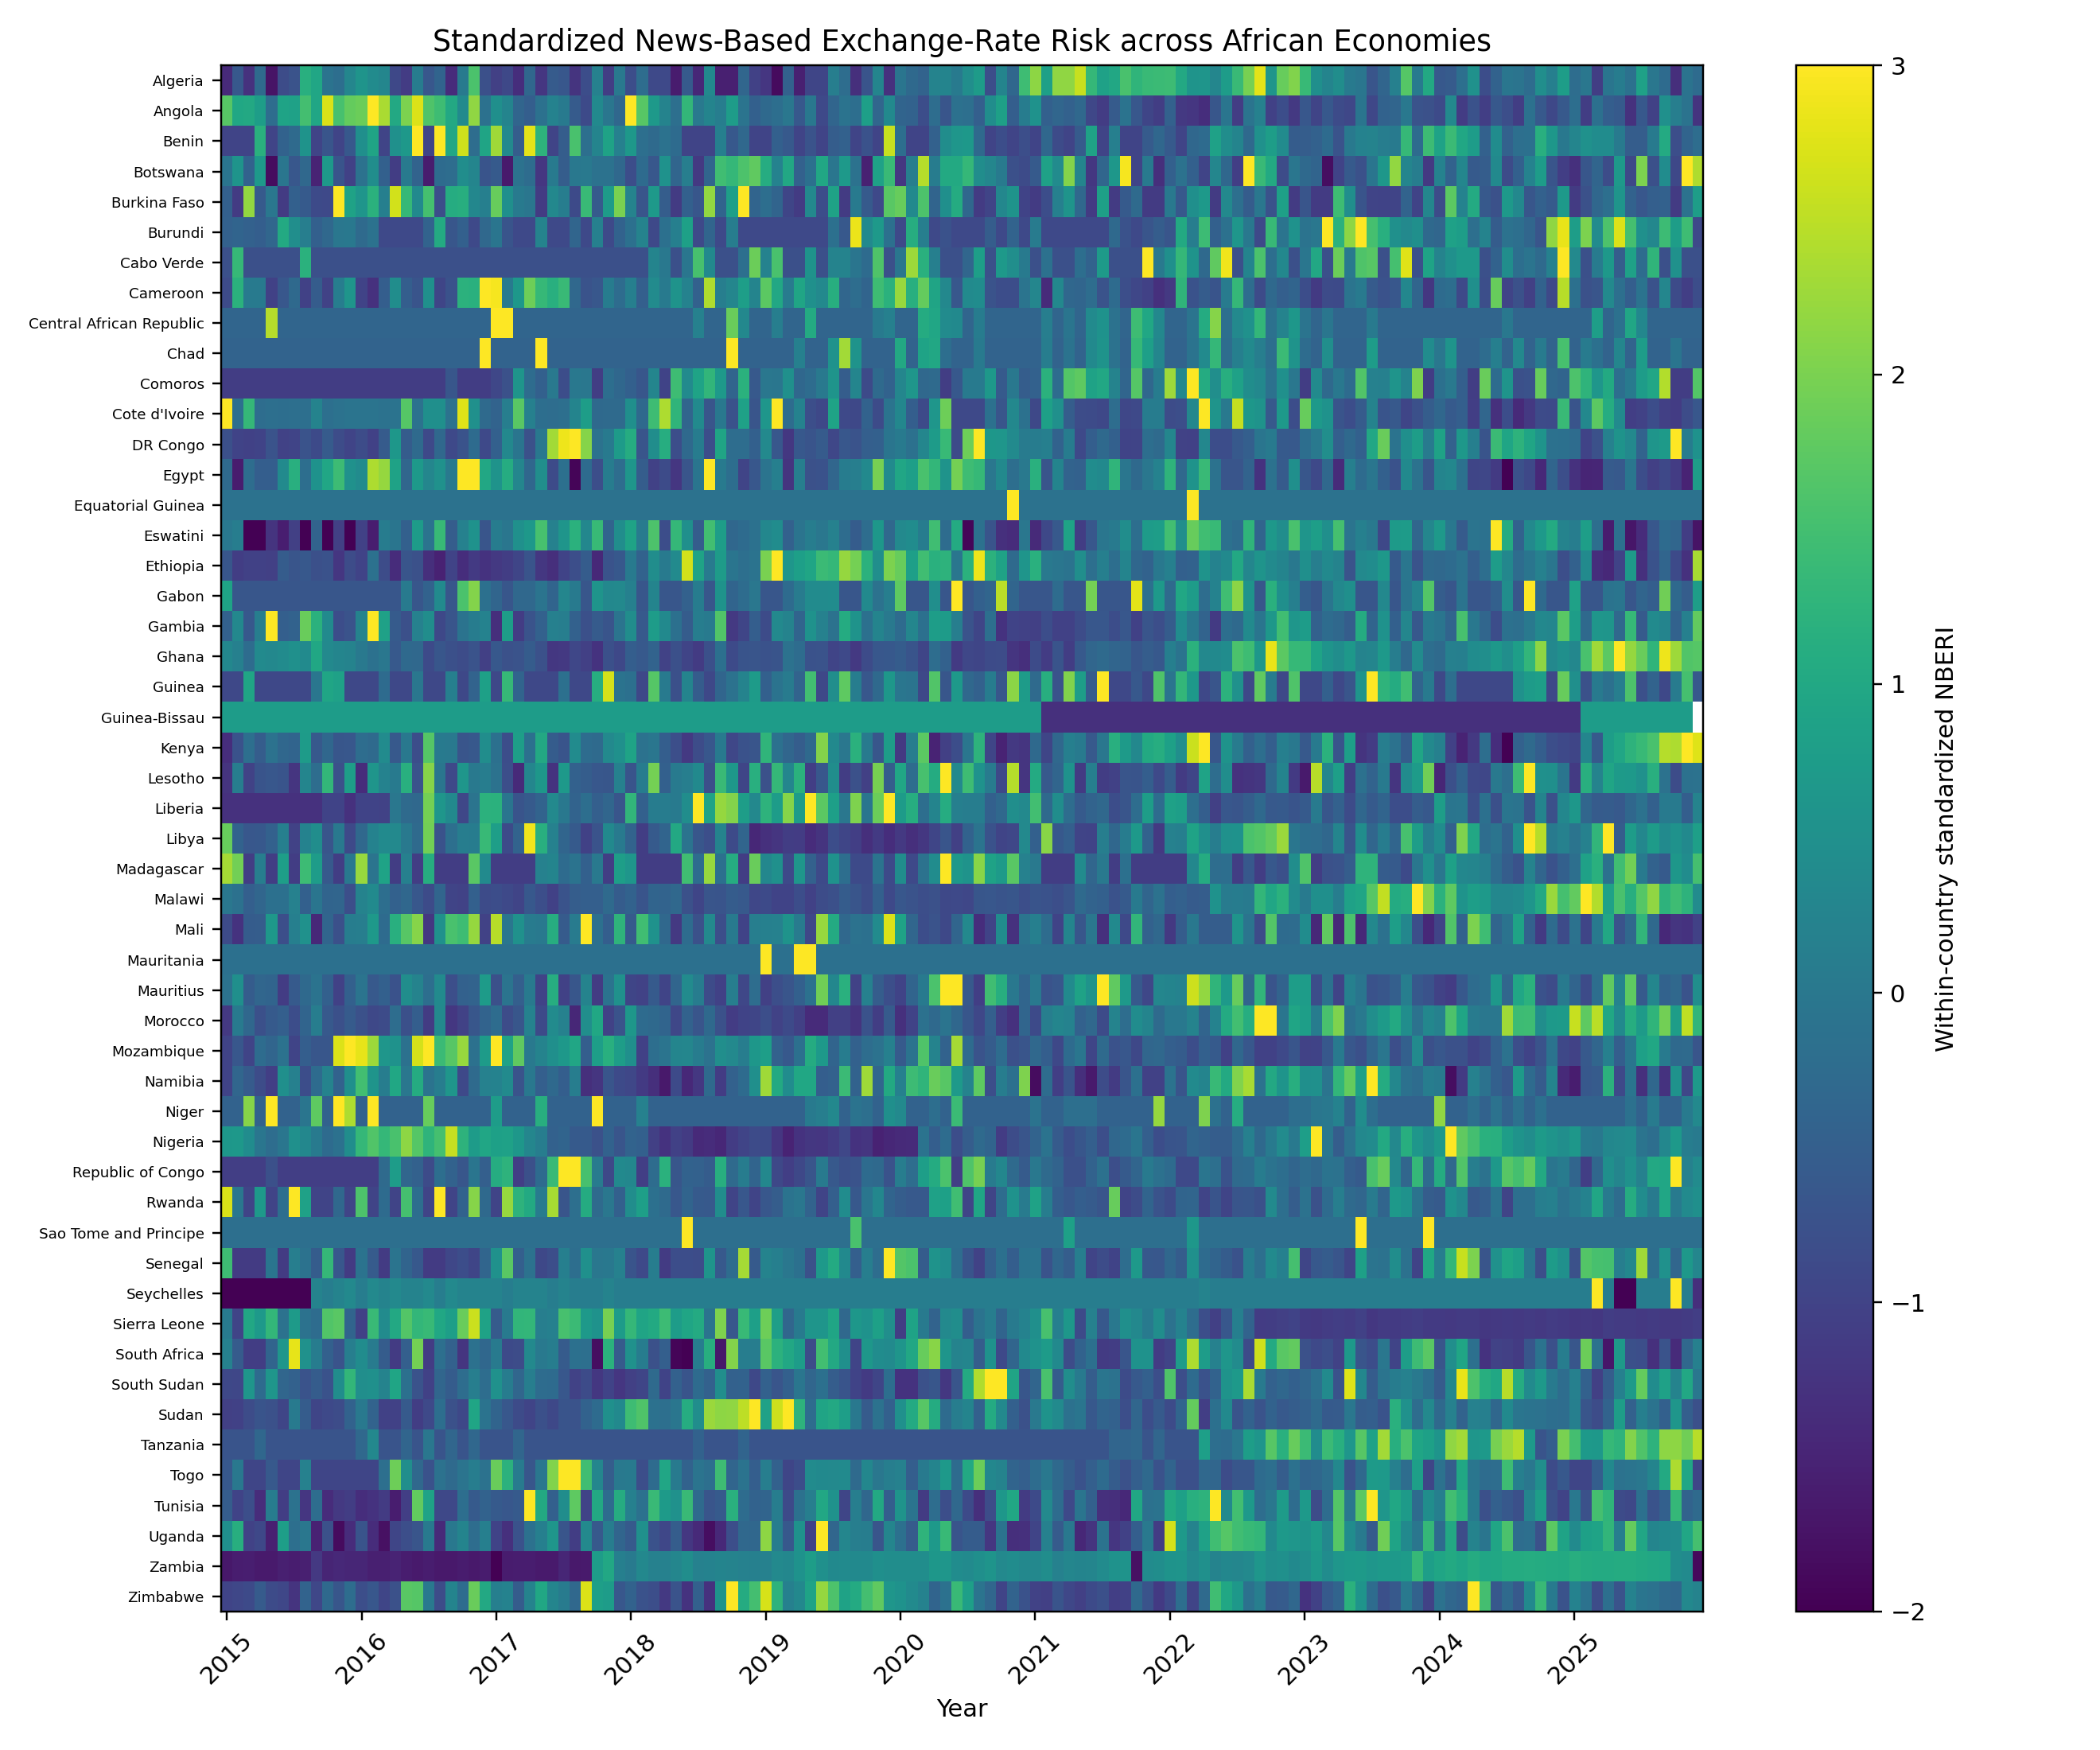
\includegraphics[width=6.45in]{figures/figure1_nberi_heatmap.png}
\caption{Standardized monthly NBERI across eligible African economies, 2015--2025.}
\label{fig:1}
\end{figure}

\subsection{Shared currencies and effective market
dependence}\label{shared-currencies-and-effective-market-dependence}

A country panel is not identical to a panel of independent currencies.
The WAEMU members in the sample share the West African CFA franc; the
CEMAC members share the Central African CFA franc; and South Africa,
Lesotho, Eswatini, and Namibia are treated as a linked Common Monetary
Area cluster for robustness. The principal regressions retain country
observations because NBERI is country-specific and the research question
concerns country risk environments. A complementary 36-cluster
specification collapses shared or linked exchange-rate paths so that the
same currency movement is not counted repeatedly as independent market
evidence. Cross-sectional dependence in the full panel is addressed
further through common time effects and Driscoll-Kraay covariance
estimation.

\subsection{Two-way fixed-effects
benchmark}\label{two-way-fixed-effects-benchmark}

The principal specification asks whether the current risk state contains
information about next-month exchange-rate instability after
conditioning on market history and inflation:

\begin{equation}
\label{eq:fe-benchmark}
v_{it}
=\alpha_i+\lambda_t+\beta\,NBERI_{i,t-1}
+\rho v_{i,t-1}+\theta r_{i,t-1}+\kappa\pi_{i,t-1}
+\varepsilon_{it}.
\end{equation}

Country effects absorb time-invariant differences in market structure,
reporting intensity, currency regime, and level effects. Calendar-time
effects absorb shocks shared across the continent. Inference uses
Driscoll-Kraay standard errors with a four-month bandwidth, allowing
heteroskedasticity, serial correlation, and broad cross-sectional
dependence. The same model is re-estimated on the 36 currency-market
clusters. A threshold extension interacts lagged NBERI with an indicator
for observations above each country\textquotesingle s 75th percentile to
test whether high-risk states amplify the slope.

\subsection{Pooled panel GARCH-X
robustness}\label{pooled-panel-garch-x-robustness}

The conditional-volatility exercise is deliberately secondary because
the available exchange-rate series are monthly. It nevertheless provides
a useful robustness test of whether NBERI shifts a common GARCH variance
recursion after volatility persistence is modeled directly. Monthly
returns are standardized within country, and the pooled likelihood
allows a common GARCH persistence structure across countries with
Student-t innovations. The nested GARCH(1,1) benchmark is

\begin{equation}
\label{eq:pooled-garch}
h_{it}^{\mathrm{GARCH}}
=\omega+\alpha\varepsilon_{i,t-1}^{2}+\beta h_{i,t-1}.
\end{equation}

The GARCH-X specification augments that recursion multiplicatively with lagged NBERI:

\begin{equation}
\label{eq:pooled-garchx}
h_{it}^{\mathrm{GARCH\text{-}X}}
=h_{it}^{\mathrm{GARCH}}
\exp\!\left(\delta\,NBERI_{i,t-1}\right).
\end{equation}

The coefficient $\delta$ is the parameter of interest. A positive
significant delta would indicate that the news-risk state shifts the
common conditional-variance recursion beyond lagged squared innovations
and lagged variance. The baseline GARCH, GARCH-X, GARCH-X with
inflation, and regional-slope GARCH-X models are compared by likelihood
and information criteria. A pooled GJR-GARCH-X specification is reported
in the appendix to test whether a common threshold response to negative
innovations is required.

\subsection{Fixed-effects panel VAR and generalized
dynamics}\label{fixed-effects-panel-var-and-generalized-dynamics}

Dynamic feedback is summarized with a parsimonious fixed-effects PVAR(1)
containing standardized NBERI, FX return, and the FX volatility proxy,
with lagged inflation as an exogenous control. Each equation includes
country and calendar-time effects:

\begin{equation}
\label{eq:pvar}
Y_{it}=A Y_{i,t-1}+B\pi_{i,t-1}+\mu_i+\tau_t+u_{it},
\qquad
Y_{it}=\begin{bmatrix}NBERI_{it}&r_{it}&v_{it}\end{bmatrix}^{\prime}.
\end{equation}

The long time dimension and 51-country cross-section make an
aggressively instrumented GMM system unnecessary for the
paper\textquotesingle s predictive purpose and would create a material
risk of instrument proliferation. Coefficient inference therefore uses
Driscoll-Kraay covariance estimates. Generalized impulse responses and
generalized forecast-error variance decompositions are computed from the
reduced-form innovation covariance matrix so that the reported dynamics
are invariant to variable ordering \citep{pesaran1998}. Confidence
bands for generalized responses use 300 country-block bootstrap
replications. Stability is evaluated from the companion-matrix
eigenvalues.

\subsection{Panel local projections}\label{panel-local-projections}

Local projections provide a complementary horizon-specific test \citep{jorda2005}. For horizons $h=0,\ldots,12$, the estimating equation is

\begin{equation}
\label{eq:local-projection}
v_{i,t+h}
=\alpha_i^{(h)}+\lambda_t^{(h)}+\beta_h\,NBERI_{i,t}
+\rho_h v_{i,t-1}+\theta_h r_{i,t-1}+\kappa_h\pi_{i,t}
+\varepsilon_{i,t+h}^{(h)}.
\end{equation}

Thus, $\beta_h$ traces the horizon-specific predictive response of the standardized volatility proxy to the current standardized NBERI state while holding fixed lagged volatility, lagged return, current inflation, country effects, and calendar-time effects. Driscoll-Kraay standard errors are used at each horizon. The coefficient sequence in Equation~\eqref{eq:local-projection} is interpreted as a predictive response profile rather than a structural causal impulse response.

\subsection{Expanding-window out-of-sample horse
race}\label{expanding-window-out-of-sample-horse-race}

The forecast experiment covers January 2023 through December 2025. Define the forecast target as $\ell_{it}\equiv\ln(0.01+r_{it}^{2})$. At each forecast origin, the benchmark and NBERI-augmented one-step-ahead forecasts can be written compactly as

\begin{equation}
\label{eq:forecast-benchmark}
\widehat{\ell}^{\mathrm{BM}}_{i,t+1\mid t}
=f\!\left(\ell_{it},\ell_{i,t-1},r_{it},\pi_{it},\pi_{i,t-1},\alpha_i\right),
\end{equation}

\begin{equation}
\label{eq:forecast-augmented}
\widehat{\ell}^{\mathrm{AUG}}_{i,t+1\mid t}
=g\!\left(\ell_{it},\ell_{i,t-1},r_{it},\pi_{it},\pi_{i,t-1},
NBERI_{it},NBERI_{i,t-1},\alpha_i\right).
\end{equation}

Here, $f(\cdot)$ and $g(\cdot)$ denote the estimated linear forecasting maps with country intercepts; Equation~\eqref{eq:forecast-augmented} nests the same market-history and inflation information set as Equation~\eqref{eq:forecast-benchmark} and adds two NBERI lags. All country standardization parameters are calculated from the training sample available at that forecast origin, preventing look-ahead contamination.\footnote{Re-estimating standardization parameters at each forecast origin is essential: using full-sample means or standard deviations would leak future information into the 2023--2025 evaluation window.} Forecasts are evaluated using RMSE and QLIKE. The Clark-West test assesses nested mean-squared predictive accuracy, and a one-sided HAC test evaluates the monthly QLIKE loss differential \citep{clark2007,patton2011}.

\subsection{Market-alignment extension and country-level
GARCH-family
design}\label{market-alignment-extension-and-country-level-garch-family-design}

The continental analysis remains the primary specification. The heterogeneity extension ranks the 51 eligible countries by the market-alignment statistic

\begin{equation}
\label{eq:alignment}
A_i
=\operatorname{Corr}\!\left(FXExternalRisk_{it},S_{it}\right),
\qquad
t\in\mathcal{T}=\{\text{2015:01},\ldots,\text{2025:12}\},
\end{equation}

where $S_{it}$ is the bilateral exchange-rate level measured as local-currency units per U.S. dollar. The 15 highest-alignment markets are Zambia, Ghana, Malawi, Tanzania, Algeria, Burundi, Libya, Nigeria, Tunisia, Morocco, Liberia, Namibia, Congo DRC, Guinea, and Benin. A positive value of $A_i$ means that elevated FX-risk narratives tend to occur when the domestic-currency price of the U.S. dollar is high; it is not a statement about next-month depreciation.\footnote{The bilateral exchange rate is measured as units of local currency per U.S. dollar. A higher level therefore denotes a larger domestic-currency price of the dollar, but the level correlation in Equation~\eqref{eq:alignment} does not by itself identify the direction or timing of subsequent depreciation.}

The level-correlation ranking is used only to organize heterogeneity. To
guard against a purely mechanical subsample story, the paper estimates
the interaction NBERI\_i,t-1 x Aligned\_i in the full eligible panel,
compares the selected-group slope with the remaining-market slope,
estimates the same interaction in the horizon-1 local projection,
evaluates a continuous NBERI-by-alignment interaction, and benchmarks
the selected-group coefficient against 1,000 random 15-country subsets.
Spearman and detrended log-exchange-rate correlations are reported as
descriptive sensitivity checks. The interaction tests, rather than the
raw ranking itself, provide the formal evidence on differential
transmission.\footnote{This distinction protects the contribution from resting mechanically on a same-sample level correlation: the ranking organizes the heterogeneity, while the interaction estimates test whether the subsequent risk-to-volatility relation actually differs.}

Within the aligned subsample, the paper reruns the fixed-effects, PVAR, generalized-response, FEVD, local-projection, forecast, absolute-return, and first-difference-NBERI exercises. Country-level conditional variance is then examined using six models: GARCH(1,1), GARCH-X, EGARCH(1,1), EGARCH-X, GJR-GARCH/TGARCH(1,1), and GJR-GARCH/TGARCH-X. Each model uses the AR(1) conditional mean

\begin{equation}
\label{eq:garch-mean}
r_{it}=\mu_i+\phi_i r_{i,t-1}+\varepsilon_{it},
\qquad
z_{it}=\frac{\varepsilon_{it}}{\sqrt{h_{it}}},
\end{equation}

with standardized Student-$t$ innovations. The NBERI-augmented GARCH(1,1) recursion is

\begin{equation}
\label{eq:garchx-country}
h_{it}
=\left(\omega_i+\alpha_i\varepsilon_{i,t-1}^{2}+\beta_i h_{i,t-1}\right)
\exp\!\left(\delta_i NBERI_{i,t-1}\right).
\end{equation}

For EGARCH-X, the log-variance recursion is

\begin{equation}
\label{eq:egarchx-country}
\begin{aligned}
\ln h_{it}
={}&\omega_i+\beta_i\ln h_{i,t-1}
+\alpha_i\!\left(|z_{i,t-1}|-\mathrm{E}|z_{i,t-1}|\right)\\
&+\gamma_i z_{i,t-1}+\delta_i NBERI_{i,t-1}.
\end{aligned}
\end{equation}

For GJR-GARCH/TGARCH-X, the threshold recursion is

\begin{equation}
\label{eq:gjrx-country}
\begin{aligned}
h_{it}
={}&\Bigl[\omega_i+
\bigl(\alpha_i+\gamma_i\mathbf{1}\{\varepsilon_{i,t-1}<0\}\bigr)
\varepsilon_{i,t-1}^{2}\\
&\qquad+\beta_i h_{i,t-1}\Bigr]
\exp\!\left(\delta_i NBERI_{i,t-1}\right).
\end{aligned}
\end{equation}

The corresponding non-X GARCH, EGARCH, and GJR/TGARCH models are obtained by imposing $\delta_i=0$. Thus, $\delta_i$ is the common object of interest across the three families: a positive value means that a higher lagged FX-risk state raises conditional variance after the family's own persistence and innovation terms have been absorbed. Likelihood-ratio tests compare each X model with its nested non-X family, and Benjamini-Hochberg q-values control multiplicity across the 15 countries within each family \citep{benjamini1995}.\footnote{Writing the three X recursions explicitly makes clear that the NBERI term is tested against different volatility dynamics: symmetric persistence in GARCH-X, logarithmic and sign-sensitive dynamics in EGARCH-X, and threshold asymmetry in GJR/TGARCH-X.}

Because nonlinear volatility likelihoods can be sensitive to starting values, the reported country-level X estimates are subjected to an explicit profile-likelihood check over the NBERI variance coefficient before joint refinement. Let $\vartheta_{-\delta}$ denote all parameters other than $\delta$. The profile estimator is

\begin{equation}
\label{eq:profile-likelihood}
\widehat{\delta}_{\mathrm{prof}}
=\arg\max_{\delta}\;
\ell\!\left(\widehat{\vartheta}_{-\delta}(\delta),\delta\right),
\qquad
\widehat{\vartheta}_{-\delta}(\delta)
=\arg\max_{\vartheta_{-\delta}}
\ell\!\left(\vartheta_{-\delta},\delta\right).
\end{equation}

The profile step in Equation~\eqref{eq:profile-likelihood} ensures that a reported X effect improves the corresponding nested family rather than reflecting a single local optimum. Residual squared-autocorrelation and ARCH-LM diagnostics are reported alongside the likelihood tests.\footnote{The country-level GARCH-family estimates use custom maximum likelihood with multiple starts, nested likelihood checks, and the explicit profile search in Equation~\eqref{eq:profile-likelihood}. Full country-family results and residual diagnostics are reported in Appendix H.}

\section{Empirical Results}\label{empirical-results}

\subsection{Continental risk variation and exchange-rate
behavior}\label{continental-risk-variation-and-exchange-rate-behavior}

The broader panel reveals pronounced heterogeneity in both news risk and
exchange-rate adjustment. NBERI is right-skewed, with a mean of 5.44, a
median of 1.64, and a maximum above 200 in the raw scale. Monthly FX
returns are likewise heavy-tailed, including infrequent but large
devaluations and re-pricing episodes. These distributional features
motivate within-country standardization in pooled models and Student-t
innovations in the conditional-volatility exercise. The heatmap in
Figure 1 also shows that elevated risk episodes are neither synchronized
across all countries nor confined to one region, supporting a design
that controls for common monthly shocks rather than attributing every
co-movement to NBERI.

\subsection{Baseline predictive relationship and shared-currency
robustness}\label{baseline-predictive-relationship-and-shared-currency-robustness}

\textbf{Table 3. Dynamic panel estimates of subsequent FX volatility}

\begingroup\footnotesize
\begin{longtable}[]{@{}
  >{\raggedright\arraybackslash}p{(\columnwidth - 12\tabcolsep) * \real{0.1429}}
  >{\raggedright\arraybackslash}p{(\columnwidth - 12\tabcolsep) * \real{0.1429}}
  >{\raggedright\arraybackslash}p{(\columnwidth - 12\tabcolsep) * \real{0.1429}}
  >{\raggedright\arraybackslash}p{(\columnwidth - 12\tabcolsep) * \real{0.1429}}
  >{\raggedright\arraybackslash}p{(\columnwidth - 12\tabcolsep) * \real{0.1429}}
  >{\raggedright\arraybackslash}p{(\columnwidth - 12\tabcolsep) * \real{0.1429}}
  >{\raggedright\arraybackslash}p{(\columnwidth - 12\tabcolsep) * \real{0.1429}}@{}}
\toprule\noalign{}
\begin{minipage}[b]{\linewidth}\raggedright
\textbf{Specification}
\end{minipage} & \begin{minipage}[b]{\linewidth}\raggedright
\textbf{Regressor}
\end{minipage} & \begin{minipage}[b]{\linewidth}\raggedright
\textbf{Coefficient}
\end{minipage} & \begin{minipage}[b]{\linewidth}\raggedright
\textbf{DK SE}
\end{minipage} & \begin{minipage}[b]{\linewidth}\raggedright
\textbf{p-value}
\end{minipage} & \begin{minipage}[b]{\linewidth}\raggedright
\textbf{N}
\end{minipage} & \begin{minipage}[b]{\linewidth}\raggedright
\textbf{Within R2}
\end{minipage} \\
\midrule\noalign{}
\endhead
\bottomrule\noalign{}
\endlastfoot
Baseline (no inflation) & Lag NBERI & 0.034 & 0.011 & 0.001 & 6,393 &
0.104 \\
Baseline (no inflation) & Lag volatility & 0.288 & 0.034 &
\textless0.001 & 6,393 & 0.104 \\
Baseline (no inflation) & Lag return & 0.067 & 0.032 & 0.034 & 6,393 &
0.104 \\
Baseline + inflation & Lag NBERI & 0.030 & 0.010 & 0.004 & 6,347 &
0.107 \\
Baseline + inflation & Lag volatility & 0.273 & 0.035 & \textless0.001 &
6,347 & 0.107 \\
Baseline + inflation & Lag return & 0.075 & 0.032 & 0.021 & 6,347 &
0.107 \\
Baseline + inflation & Lag inflation & 0.073 & 0.019 & \textless0.001 &
6,347 & 0.107 \\
Currency-cluster robustness & Lag NBERI & 0.033 & 0.013 & 0.011 & 4,406
& 0.154 \\
Currency-cluster robustness & Lag volatility & 0.333 & 0.026 &
\textless0.001 & 4,406 & 0.154 \\
Currency-cluster robustness & Lag return & 0.069 & 0.029 & 0.018 & 4,406
& 0.154 \\
Currency-cluster robustness & Lag inflation & 0.087 & 0.021 &
\textless0.001 & 4,406 & 0.154 \\
\end{longtable}
\endgroup

\textbf{Notes:} Dependent variable is the within-country standardized
monthly volatility proxy. All specifications include country and
calendar-time effects. The currency-cluster model uses 36 market
clusters rather than 51 country series. Driscoll-Kraay bandwidth = 4.

The main result is positive and precisely estimated. In the
specification that includes inflation, lagged NBERI has a coefficient of
0.030 (Driscoll-Kraay SE = 0.010; p = 0.004). A one-standard-deviation
increase in the country-specific risk state is therefore followed by
approximately 0.03 standard deviations more exchange-rate volatility in
the next month, conditional on prior volatility, prior returns,
inflation, country effects, and common time shocks. The effect is
smaller than the autoregressive volatility coefficient (0.273), which is
consistent with NBERI adding information rather than dominating market
history.

The shared-currency robustness is central to interpretation. Once common
or tightly linked currency paths are collapsed to 36 market clusters,
the NBERI coefficient is 0.033 (SE = 0.013; p = 0.011). The estimated
relationship therefore does not depend on treating the same CFA or
Common Monetary Area exchange-rate path as multiple independent market
realizations. Lagged inflation also remains positive, and lagged returns
retain incremental information.

\subsection{Regional heterogeneity and nonlinear risk
states}\label{regional-heterogeneity-and-nonlinear-risk-states}

\textbf{Table 4. Regional NBERI slopes and high-risk threshold test}

\begingroup\footnotesize
\begin{longtable}[]{@{}
  >{\raggedright\arraybackslash}p{(\columnwidth - 6\tabcolsep) * \real{0.2500}}
  >{\raggedright\arraybackslash}p{(\columnwidth - 6\tabcolsep) * \real{0.2500}}
  >{\raggedright\arraybackslash}p{(\columnwidth - 6\tabcolsep) * \real{0.2500}}
  >{\raggedright\arraybackslash}p{(\columnwidth - 6\tabcolsep) * \real{0.2500}}@{}}
\toprule\noalign{}
\begin{minipage}[b]{\linewidth}\raggedright
\textbf{Region / threshold term}
\end{minipage} & \begin{minipage}[b]{\linewidth}\raggedright
\textbf{Coefficient}
\end{minipage} & \begin{minipage}[b]{\linewidth}\raggedright
\textbf{DK SE}
\end{minipage} & \begin{minipage}[b]{\linewidth}\raggedright
\textbf{p-value}
\end{minipage} \\
\midrule\noalign{}
\endhead
\bottomrule\noalign{}
\endlastfoot
North & 0.090 & 0.032 & 0.005 \\
West & 0.021 & 0.020 & 0.292 \\
Central & -0.004 & 0.020 & 0.839 \\
East & 0.014 & 0.023 & 0.543 \\
Southern & 0.065 & 0.032 & 0.042 \\
Wald: equality of five regional slopes & 6.217 & df = 4 & 0.184 \\
Lag NBERI below country q75 & 0.050 & 0.024 & 0.036 \\
Increment above country q75 & -0.030 & 0.031 & 0.339 \\
Total high-risk slope & 0.020 & 0.014 & 0.149 \\
\end{longtable}
\endgroup

\textbf{Notes:} Regional slopes are estimated jointly with the same
dynamic controls, country effects, and time effects as the baseline
model. The Wald row tests equality of all five regional NBERI slopes.
The threshold is each country\textquotesingle s 75th percentile of
NBERI.

\begin{figure}[!htbp]
\centering
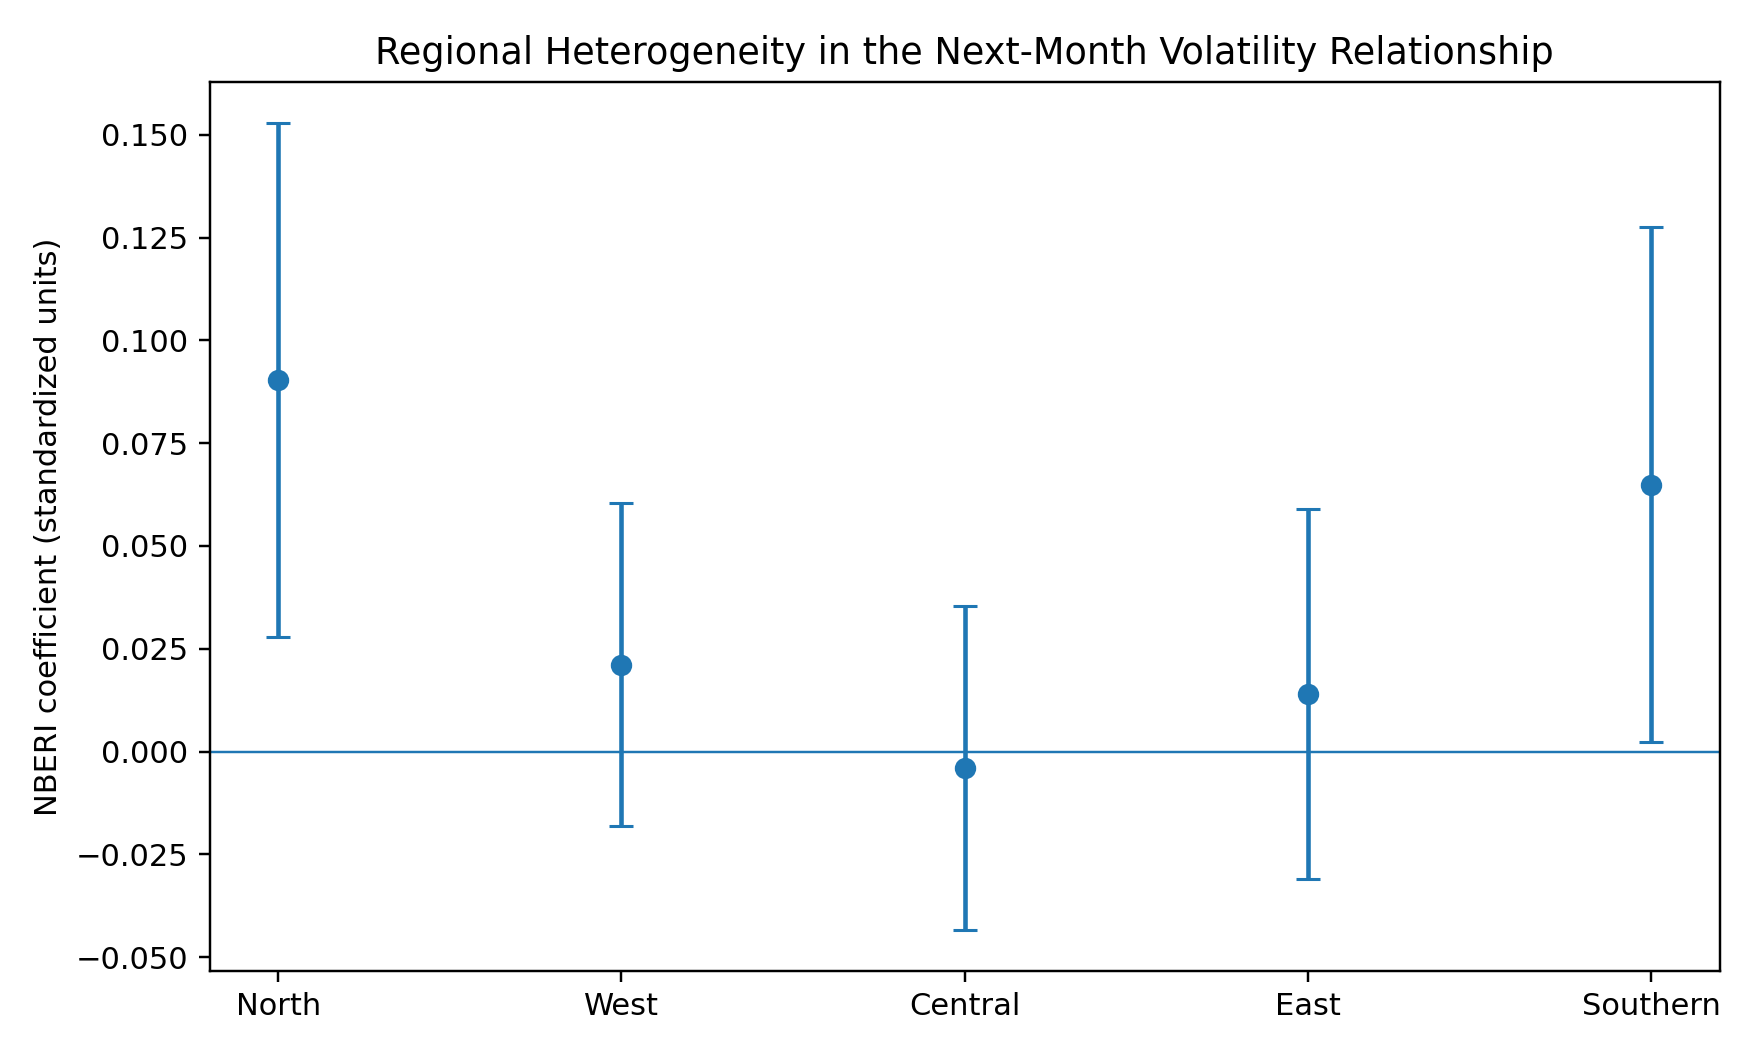
\includegraphics[width=5.9in]{figures/figure2_regional_heterogeneity.png}
\caption{Regional heterogeneity in the next-month NBERI--volatility relationship.}
\label{fig:2}
\end{figure}

North Africa (0.090, p = 0.005) and Southern Africa (0.065, p = 0.042)
have positive individual slopes, whereas the West, Central, and East
estimates are not individually significant. Those point estimates do not
establish statistically different regional mechanisms: the joint Wald
test of equality across the five regional slopes has p = 0.184. The
paper therefore treats the regional pattern as descriptive heterogeneity
rather than evidence of separate structural transmission regimes.

The high-risk threshold model also argues against a crisis-amplification
narrative. Below the country-specific 75th percentile, the NBERI slope
is 0.050 (p = 0.036). The incremental slope above the threshold is
-0.030 (p = 0.339), and the total high-risk slope is not significant (p
= 0.149). There is no evidence that the predictive relationship becomes
systematically stronger once NBERI crosses the high-risk threshold.

\subsection{Pooled panel GARCH-X: a stricter conditional-variance
test}\label{pooled-panel-garch-x-a-stricter-conditional-variance-test}

\textbf{Table 5. Pooled monthly panel GARCH-X results}

\begingroup\footnotesize
\begin{longtable}[]{@{}
  >{\raggedright\arraybackslash}p{(\columnwidth - 12\tabcolsep) * \real{0.1429}}
  >{\raggedright\arraybackslash}p{(\columnwidth - 12\tabcolsep) * \real{0.1429}}
  >{\raggedright\arraybackslash}p{(\columnwidth - 12\tabcolsep) * \real{0.1429}}
  >{\raggedright\arraybackslash}p{(\columnwidth - 12\tabcolsep) * \real{0.1429}}
  >{\raggedright\arraybackslash}p{(\columnwidth - 12\tabcolsep) * \real{0.1429}}
  >{\raggedright\arraybackslash}p{(\columnwidth - 12\tabcolsep) * \real{0.1429}}
  >{\raggedright\arraybackslash}p{(\columnwidth - 12\tabcolsep) * \real{0.1429}}@{}}
\toprule\noalign{}
\begin{minipage}[b]{\linewidth}\raggedright
\textbf{Model}
\end{minipage} & \begin{minipage}[b]{\linewidth}\raggedright
\textbf{Parameter}
\end{minipage} & \begin{minipage}[b]{\linewidth}\raggedright
\textbf{Estimate}
\end{minipage} & \begin{minipage}[b]{\linewidth}\raggedright
\textbf{SE}
\end{minipage} & \begin{minipage}[b]{\linewidth}\raggedright
\textbf{p-value}
\end{minipage} & \begin{minipage}[b]{\linewidth}\raggedright
\textbf{AIC}
\end{minipage} & \begin{minipage}[b]{\linewidth}\raggedright
\textbf{BIC}
\end{minipage} \\
\midrule\noalign{}
\endhead
\bottomrule\noalign{}
\endlastfoot
Panel GARCH & alpha + beta & 0.995 & & & 14985.0 & 15012.1 \\
Panel GARCH-X & NBERI & -0.0046 & 0.0106 & 0.663 & 14986.8 & 15020.7 \\
Panel GARCH-X + inflation & NBERI & -0.0049 & 0.0107 & 0.647 & 14988.8 &
15029.4 \\
Regional GARCH-X: North & NBERI & 0.0120 & 0.0258 & 0.641 & & \\
Regional GARCH-X: West & NBERI & -0.0170 & 0.0197 & 0.388 & & \\
Regional GARCH-X: Central & NBERI & -0.0520 & 0.0301 & 0.084 & & \\
Regional GARCH-X: East & NBERI & 0.0197 & 0.0225 & 0.381 & & \\
Regional GARCH-X: Southern & NBERI & 0.0033 & 0.0243 & 0.891 & & \\
\end{longtable}
\endgroup

\textbf{Notes:} Likelihood-ratio test for GARCH versus GARCH-X: LR =
0.191, p = 0.662. Test of common versus regional NBERI variance
parameters: LR = 4.644, p = 0.326. Models use within-country
standardized monthly returns and Student-t innovations.

\begin{figure}[!htbp]
\centering
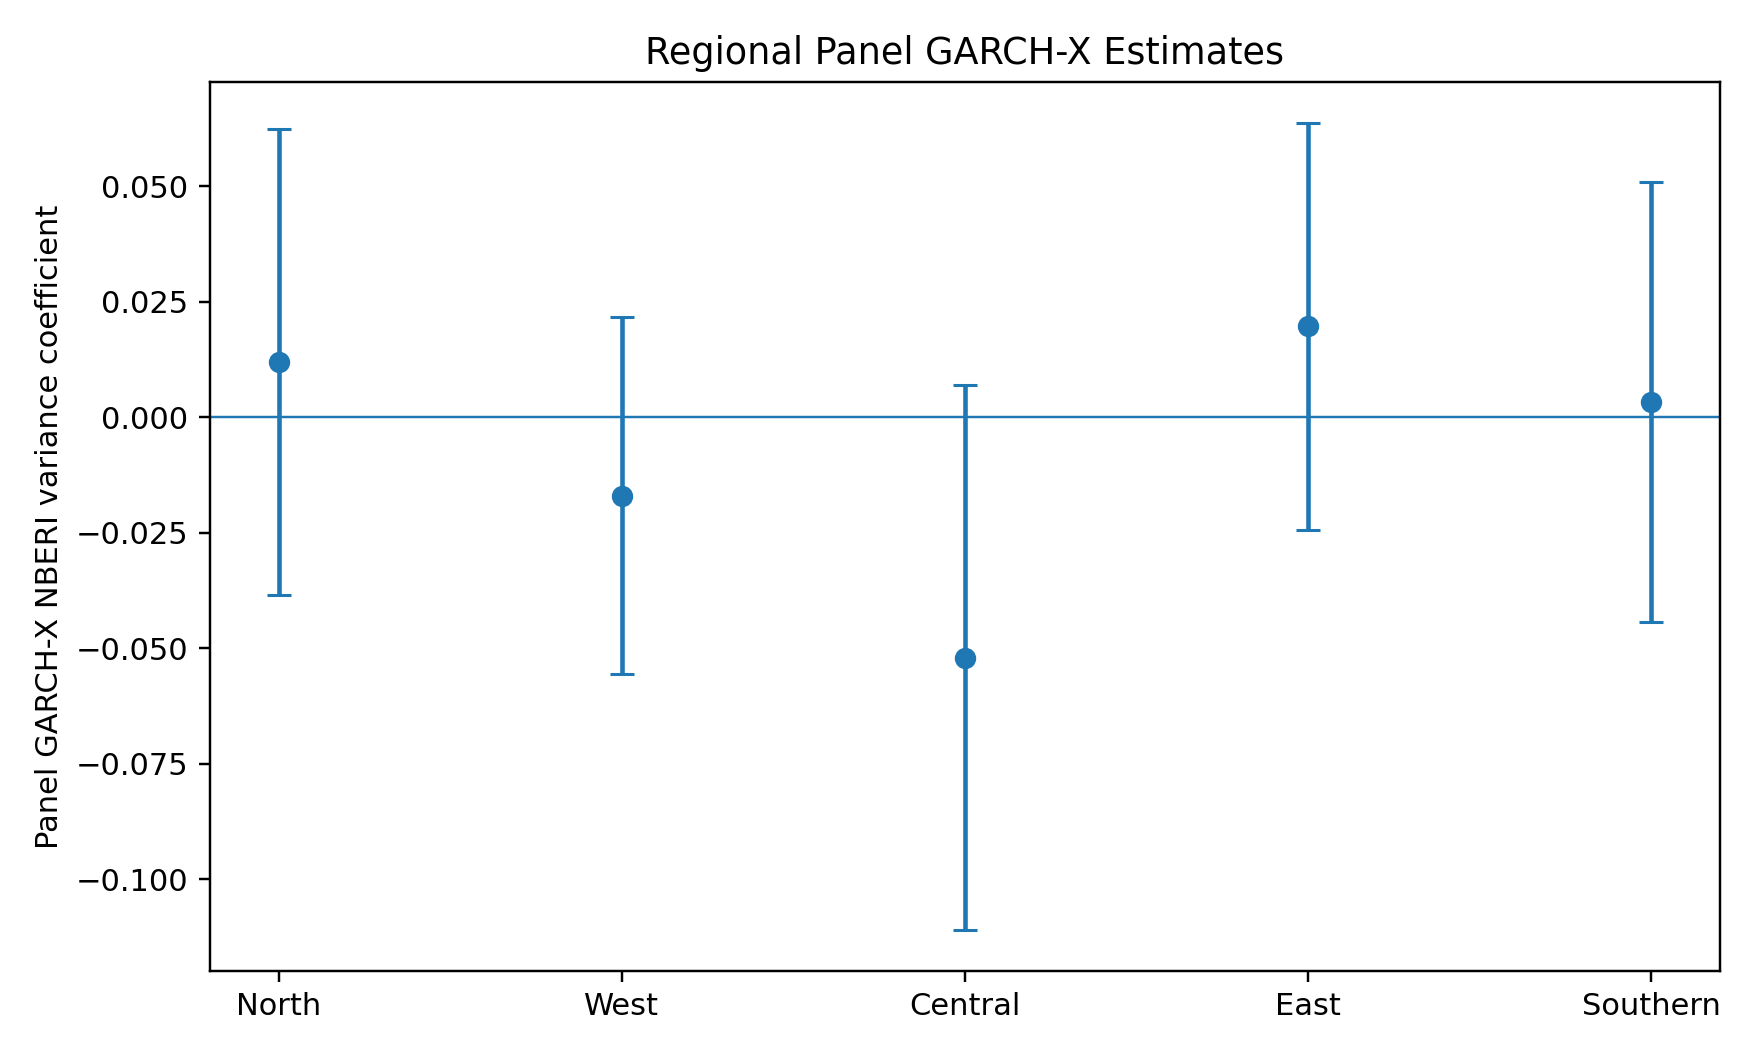
\includegraphics[width=5.9in]{figures/figure3_pooled_garch_regions.png}
\caption{Regional NBERI coefficients in the pooled monthly panel GARCH-X model.}
\label{fig:3}
\end{figure}

The panel GARCH exercise produces a materially different result from the
two-way fixed-effects model. Monthly conditional variance is highly
persistent: alpha + beta is approximately 0.995. Once that recursion is
absorbed, however, the common NBERI variance coefficient is -0.0046 (p =
0.663). The likelihood-ratio test comparing GARCH with GARCH-X is also
insignificant (p = 0.662), and AIC and BIC do not favor the
NBERI-augmented model. Adding inflation does not change the conclusion.
Regional GARCH-X coefficients are individually insignificant, and the
common-versus-regional likelihood-ratio test has p = 0.326.

This result narrows the mechanism supported by the data. The
fixed-effects model asks whether the monthly risk state contains
information about the next month\textquotesingle s observed
exchange-rate movement after controls. The GARCH-X model asks whether
NBERI shifts a common parametric variance recursion after lagged
variance and squared innovations have absorbed nearly all persistence.
The data support the former relationship, not the latter. Treating those
tests as interchangeable would overstate the evidence.

\subsection{Dynamic feedback: PVAR, generalized responses, and
variance
decomposition}\label{dynamic-feedback-pvar-generalized-responses-and-variance-decomposition}

\textbf{Table 6. Fixed-effects PVAR(1) coefficients}

\begingroup\footnotesize
\begin{longtable}[]{@{}
  >{\raggedright\arraybackslash}p{(\columnwidth - 8\tabcolsep) * \real{0.2000}}
  >{\raggedright\arraybackslash}p{(\columnwidth - 8\tabcolsep) * \real{0.2000}}
  >{\raggedright\arraybackslash}p{(\columnwidth - 8\tabcolsep) * \real{0.2000}}
  >{\raggedright\arraybackslash}p{(\columnwidth - 8\tabcolsep) * \real{0.2000}}
  >{\raggedright\arraybackslash}p{(\columnwidth - 8\tabcolsep) * \real{0.2000}}@{}}
\toprule\noalign{}
\begin{minipage}[b]{\linewidth}\raggedright
\textbf{Equation}
\end{minipage} & \begin{minipage}[b]{\linewidth}\raggedright
\textbf{Lagged regressor}
\end{minipage} & \begin{minipage}[b]{\linewidth}\raggedright
\textbf{Coefficient}
\end{minipage} & \begin{minipage}[b]{\linewidth}\raggedright
\textbf{DK SE}
\end{minipage} & \begin{minipage}[b]{\linewidth}\raggedright
\textbf{p-value}
\end{minipage} \\
\midrule\noalign{}
\endhead
\bottomrule\noalign{}
\endlastfoot
NBERI & Lag NBERI & 0.366 & 0.019 & \textless0.001 \\
NBERI & Lag FX return & 0.038 & 0.017 & 0.023 \\
NBERI & Lag FX volatility & 0.036 & 0.017 & 0.031 \\
NBERI & Lag inflation & 0.020 & 0.013 & 0.109 \\
FX return & Lag NBERI & 0.025 & 0.010 & 0.016 \\
FX return & Lag FX return & 0.295 & 0.027 & \textless0.001 \\
FX return & Lag FX volatility & -0.004 & 0.030 & 0.881 \\
FX return & Lag inflation & 0.000 & 0.020 & 0.995 \\
FX volatility & Lag NBERI & 0.030 & 0.010 & 0.004 \\
FX volatility & Lag FX return & 0.075 & 0.032 & 0.022 \\
FX volatility & Lag FX volatility & 0.273 & 0.035 & \textless0.001 \\
FX volatility & Lag inflation & 0.073 & 0.019 & \textless0.001 \\
\end{longtable}
\endgroup

\textbf{Notes:} All variables are standardized within country. Country
and calendar-time effects are included in every equation; lagged
inflation enters as a control. Maximum companion-root modulus = 0.390,
satisfying the stability condition.

The PVAR reinforces the one-step panel result while clarifying feedback.
Lagged NBERI predicts the FX volatility equation with a coefficient of
0.030 (p = 0.004), essentially matching the baseline fixed-effects
estimate. NBERI also predicts next-month FX returns (0.025, p = 0.016).
In the NBERI equation, lagged FX return and lagged FX volatility are
both positive and significant at conventional levels, indicating
feedback in the information environment rather than a strictly
one-directional system. The NBERI autoregressive coefficient is 0.366,
confirming persistence without approaching a unit root in the estimated
transition matrix.

\begin{figure}[!htbp]
\centering
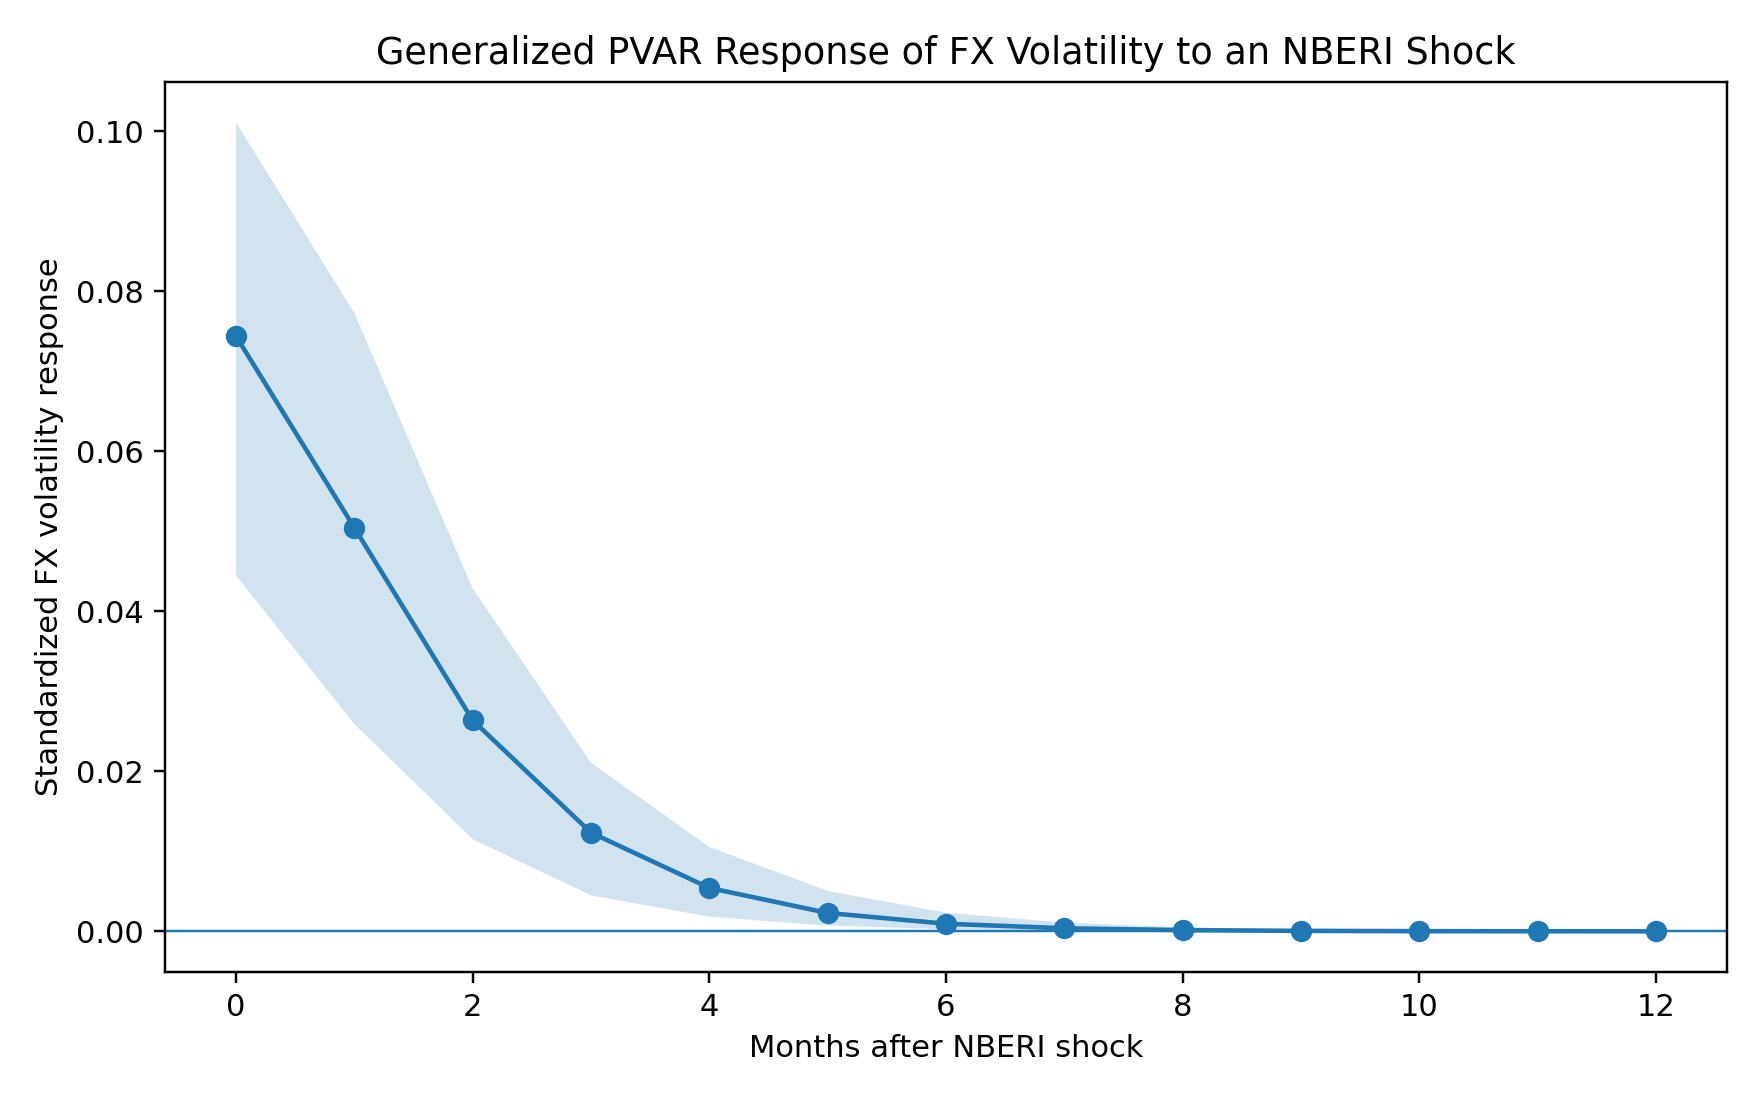
\includegraphics[width=5.75in]{figures/figure4_pvar_girf.png}
\caption{Generalized PVAR response of FX volatility to an NBERI innovation.}
\label{fig:4}
\end{figure}

The generalized response is positive on impact and decays quickly. At
horizon 1 the standardized volatility response is 0.050, with a 95
percent country-block bootstrap interval of approximately 0.026 to
0.077. At horizon 2 the response is 0.026, with an interval of roughly
0.012 to 0.043. The profile approaches zero thereafter. Because the
generalized response is derived from the reduced-form covariance matrix,
it is best read as dynamic propagation conditional on the system rather
than as the effect of an externally identified structural shock.

\begin{figure}[!htbp]
\centering
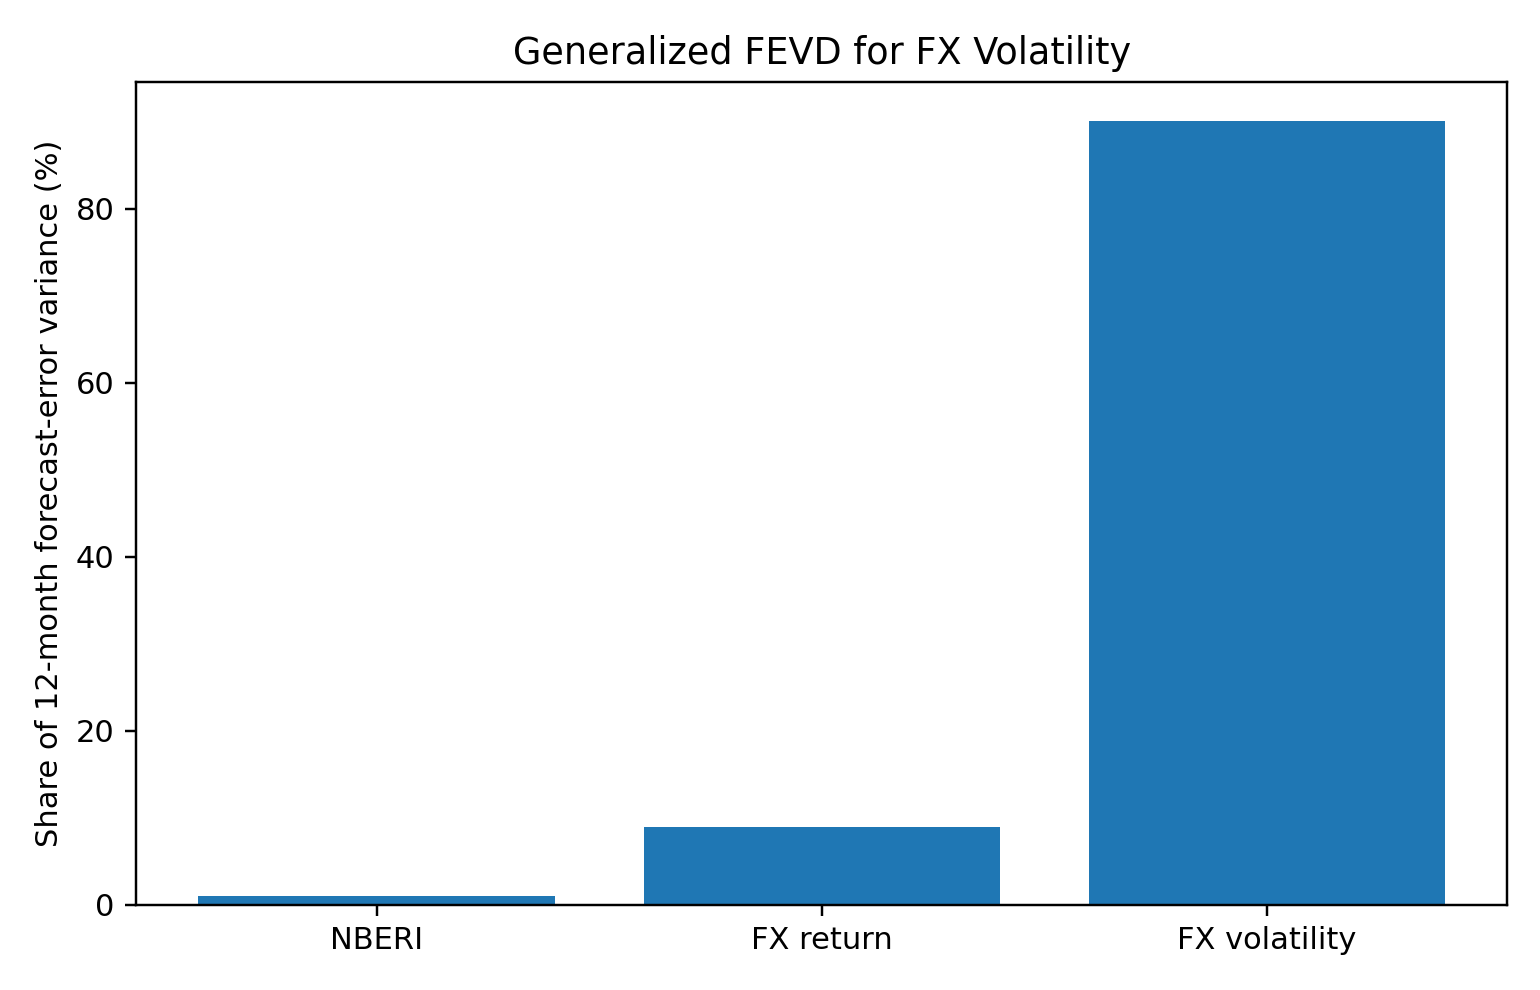
\includegraphics[width=5.45in]{figures/figure5_fevd.png}
\caption{Generalized 12-month forecast-error variance decomposition for FX volatility.}
\label{fig:5}
\end{figure}

The variance decomposition puts the size of the NBERI channel into
perspective. At a 12-month horizon, NBERI innovations account for
approximately 1.05 percent of the forecast-error variance of FX
volatility, compared with 8.90 percent for FX-return innovations and
90.04 percent for volatility\textquotesingle s own innovations. NBERI
therefore carries statistically detectable leading information, but it
is not the dominant source of exchange-rate volatility variation.

\subsection{Local-projection response
profile}\label{local-projection-response-profile}

\begin{figure}[!htbp]
\centering
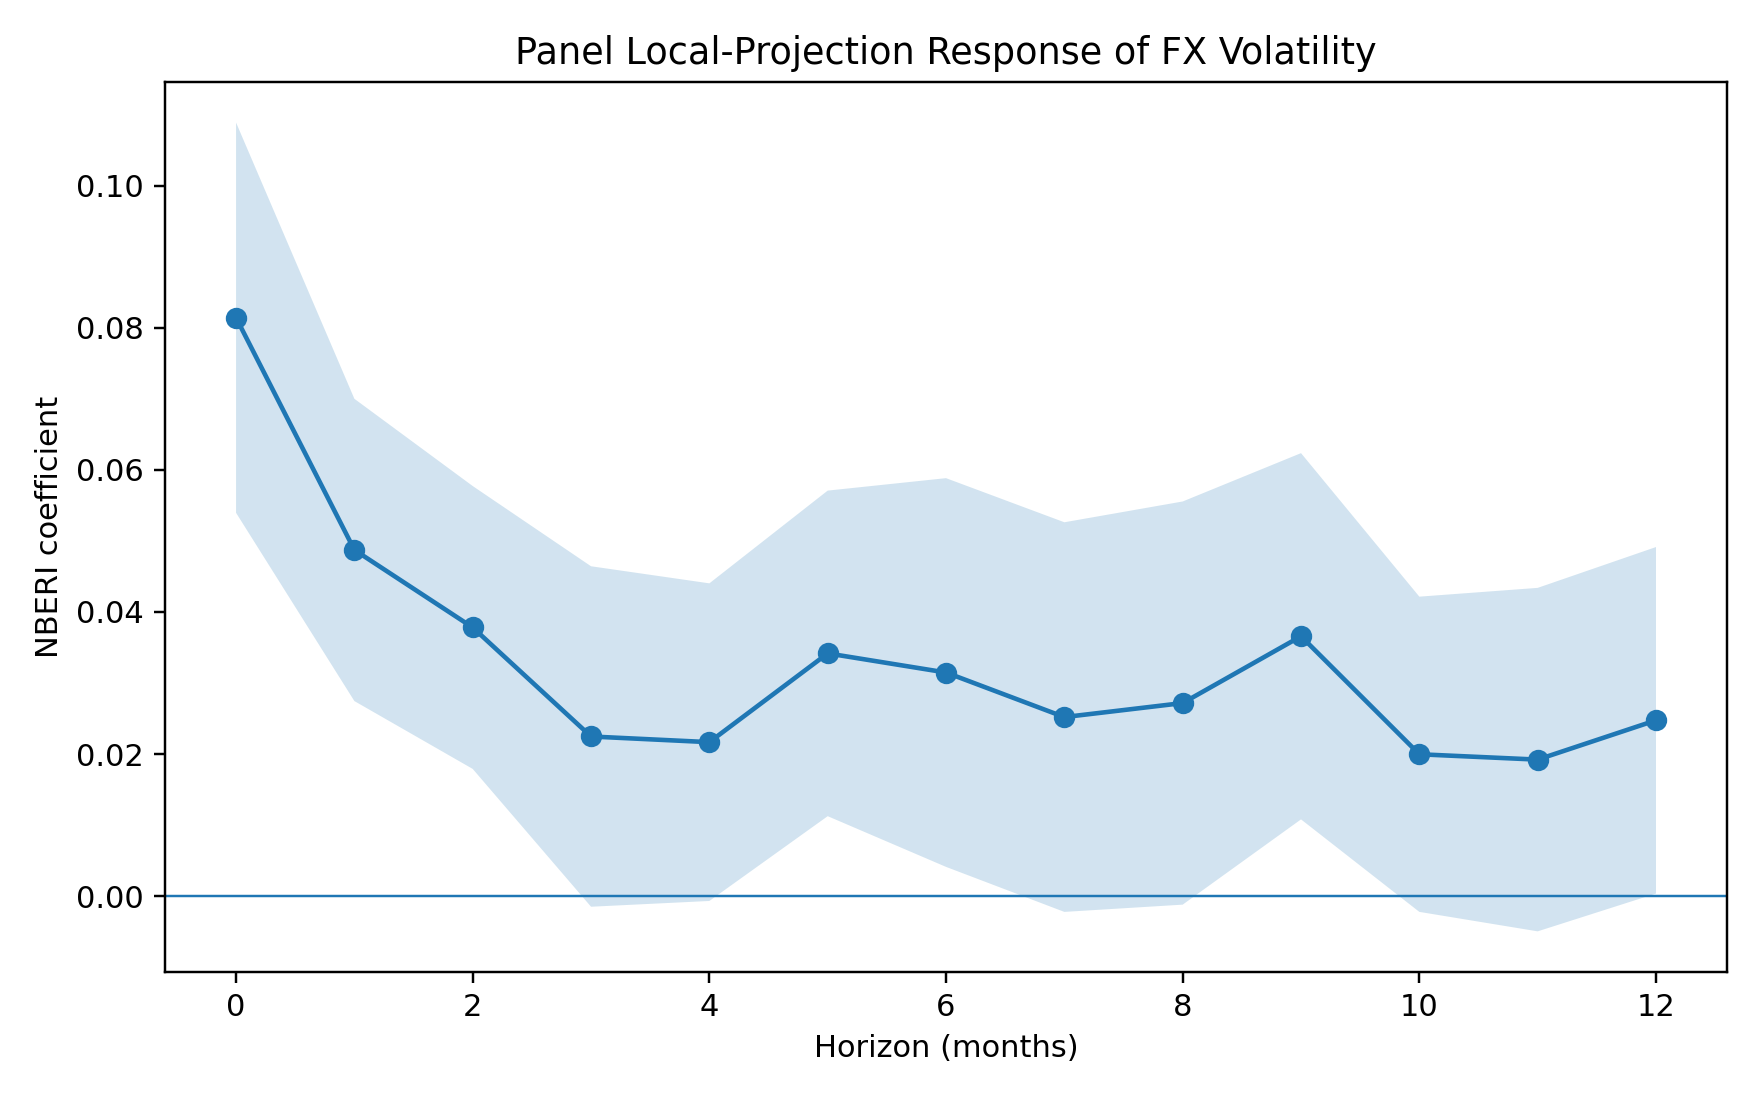
\includegraphics[width=5.85in]{figures/figure6_local_projection_continental.png}
\caption{Panel local-projection response of the monthly FX volatility proxy to NBERI.}
\label{fig:6}
\end{figure}

Local projections yield the same short-horizon direction without
requiring recursive PVAR propagation. The horizon-1 coefficient is 0.049
(p \textless{} 0.001), and the horizon-2 coefficient is 0.038 (p
\textless{} 0.001). The response is smaller and less precise at horizons
3 and 4, becomes positive and significant again at several later
horizons, and remains modest throughout. The profile is therefore not a
smooth geometric decay. The most defensible interpretation is an
immediate and near-term predictive relationship with weaker,
non-monotonic persistence at longer horizons.

\subsection{Out-of-sample predictive
content}\label{out-of-sample-predictive-content}

\textbf{Table 7. Expanding-window forecast horse race, 2023-2025}

\begingroup\footnotesize
\begin{longtable}[]{@{}
  >{\raggedright\arraybackslash}p{(\columnwidth - 10\tabcolsep) * \real{0.1667}}
  >{\raggedright\arraybackslash}p{(\columnwidth - 10\tabcolsep) * \real{0.1667}}
  >{\raggedright\arraybackslash}p{(\columnwidth - 10\tabcolsep) * \real{0.1667}}
  >{\raggedright\arraybackslash}p{(\columnwidth - 10\tabcolsep) * \real{0.1667}}
  >{\raggedright\arraybackslash}p{(\columnwidth - 10\tabcolsep) * \real{0.1667}}
  >{\raggedright\arraybackslash}p{(\columnwidth - 10\tabcolsep) * \real{0.1667}}@{}}
\toprule\noalign{}
\begin{minipage}[b]{\linewidth}\raggedright
\textbf{Result}
\end{minipage} & \begin{minipage}[b]{\linewidth}\raggedright
\textbf{Statistic}
\end{minipage} & \begin{minipage}[b]{\linewidth}\raggedright
\textbf{RMSE / mean}
\end{minipage} & \begin{minipage}[b]{\linewidth}\raggedright
\textbf{QLIKE}
\end{minipage} & \begin{minipage}[b]{\linewidth}\raggedright
\textbf{Improvement}
\end{minipage} & \begin{minipage}[b]{\linewidth}\raggedright
\textbf{p-value}
\end{minipage} \\
\midrule\noalign{}
\endhead
\bottomrule\noalign{}
\endlastfoot
Pooled benchmark & & 2.029 & 32.702 & & \\
Pooled + NBERI & & 2.025 & 31.615 & 0.20\% & \\
Clark-West nested test & Mean statistic & 0.026 & & & 0.001 \\
QLIKE loss-difference test & Baseline - NBERI & 1.050 & & &
\textless0.001 \\
Country distribution & 23 of 43 positive QLIKE gains & & & 53.5\% & \\
\end{longtable}
\endgroup

\textbf{Notes:} The benchmark uses two lags of the log variance proxy,
lagged FX return, two lags of inflation, and country intercepts. The
augmented model adds two lags of NBERI. Standardization parameters are
estimated using training data only at each forecast origin. Country
distribution includes markets with at least 24 forecast observations.

\begin{figure}[!htbp]
\centering
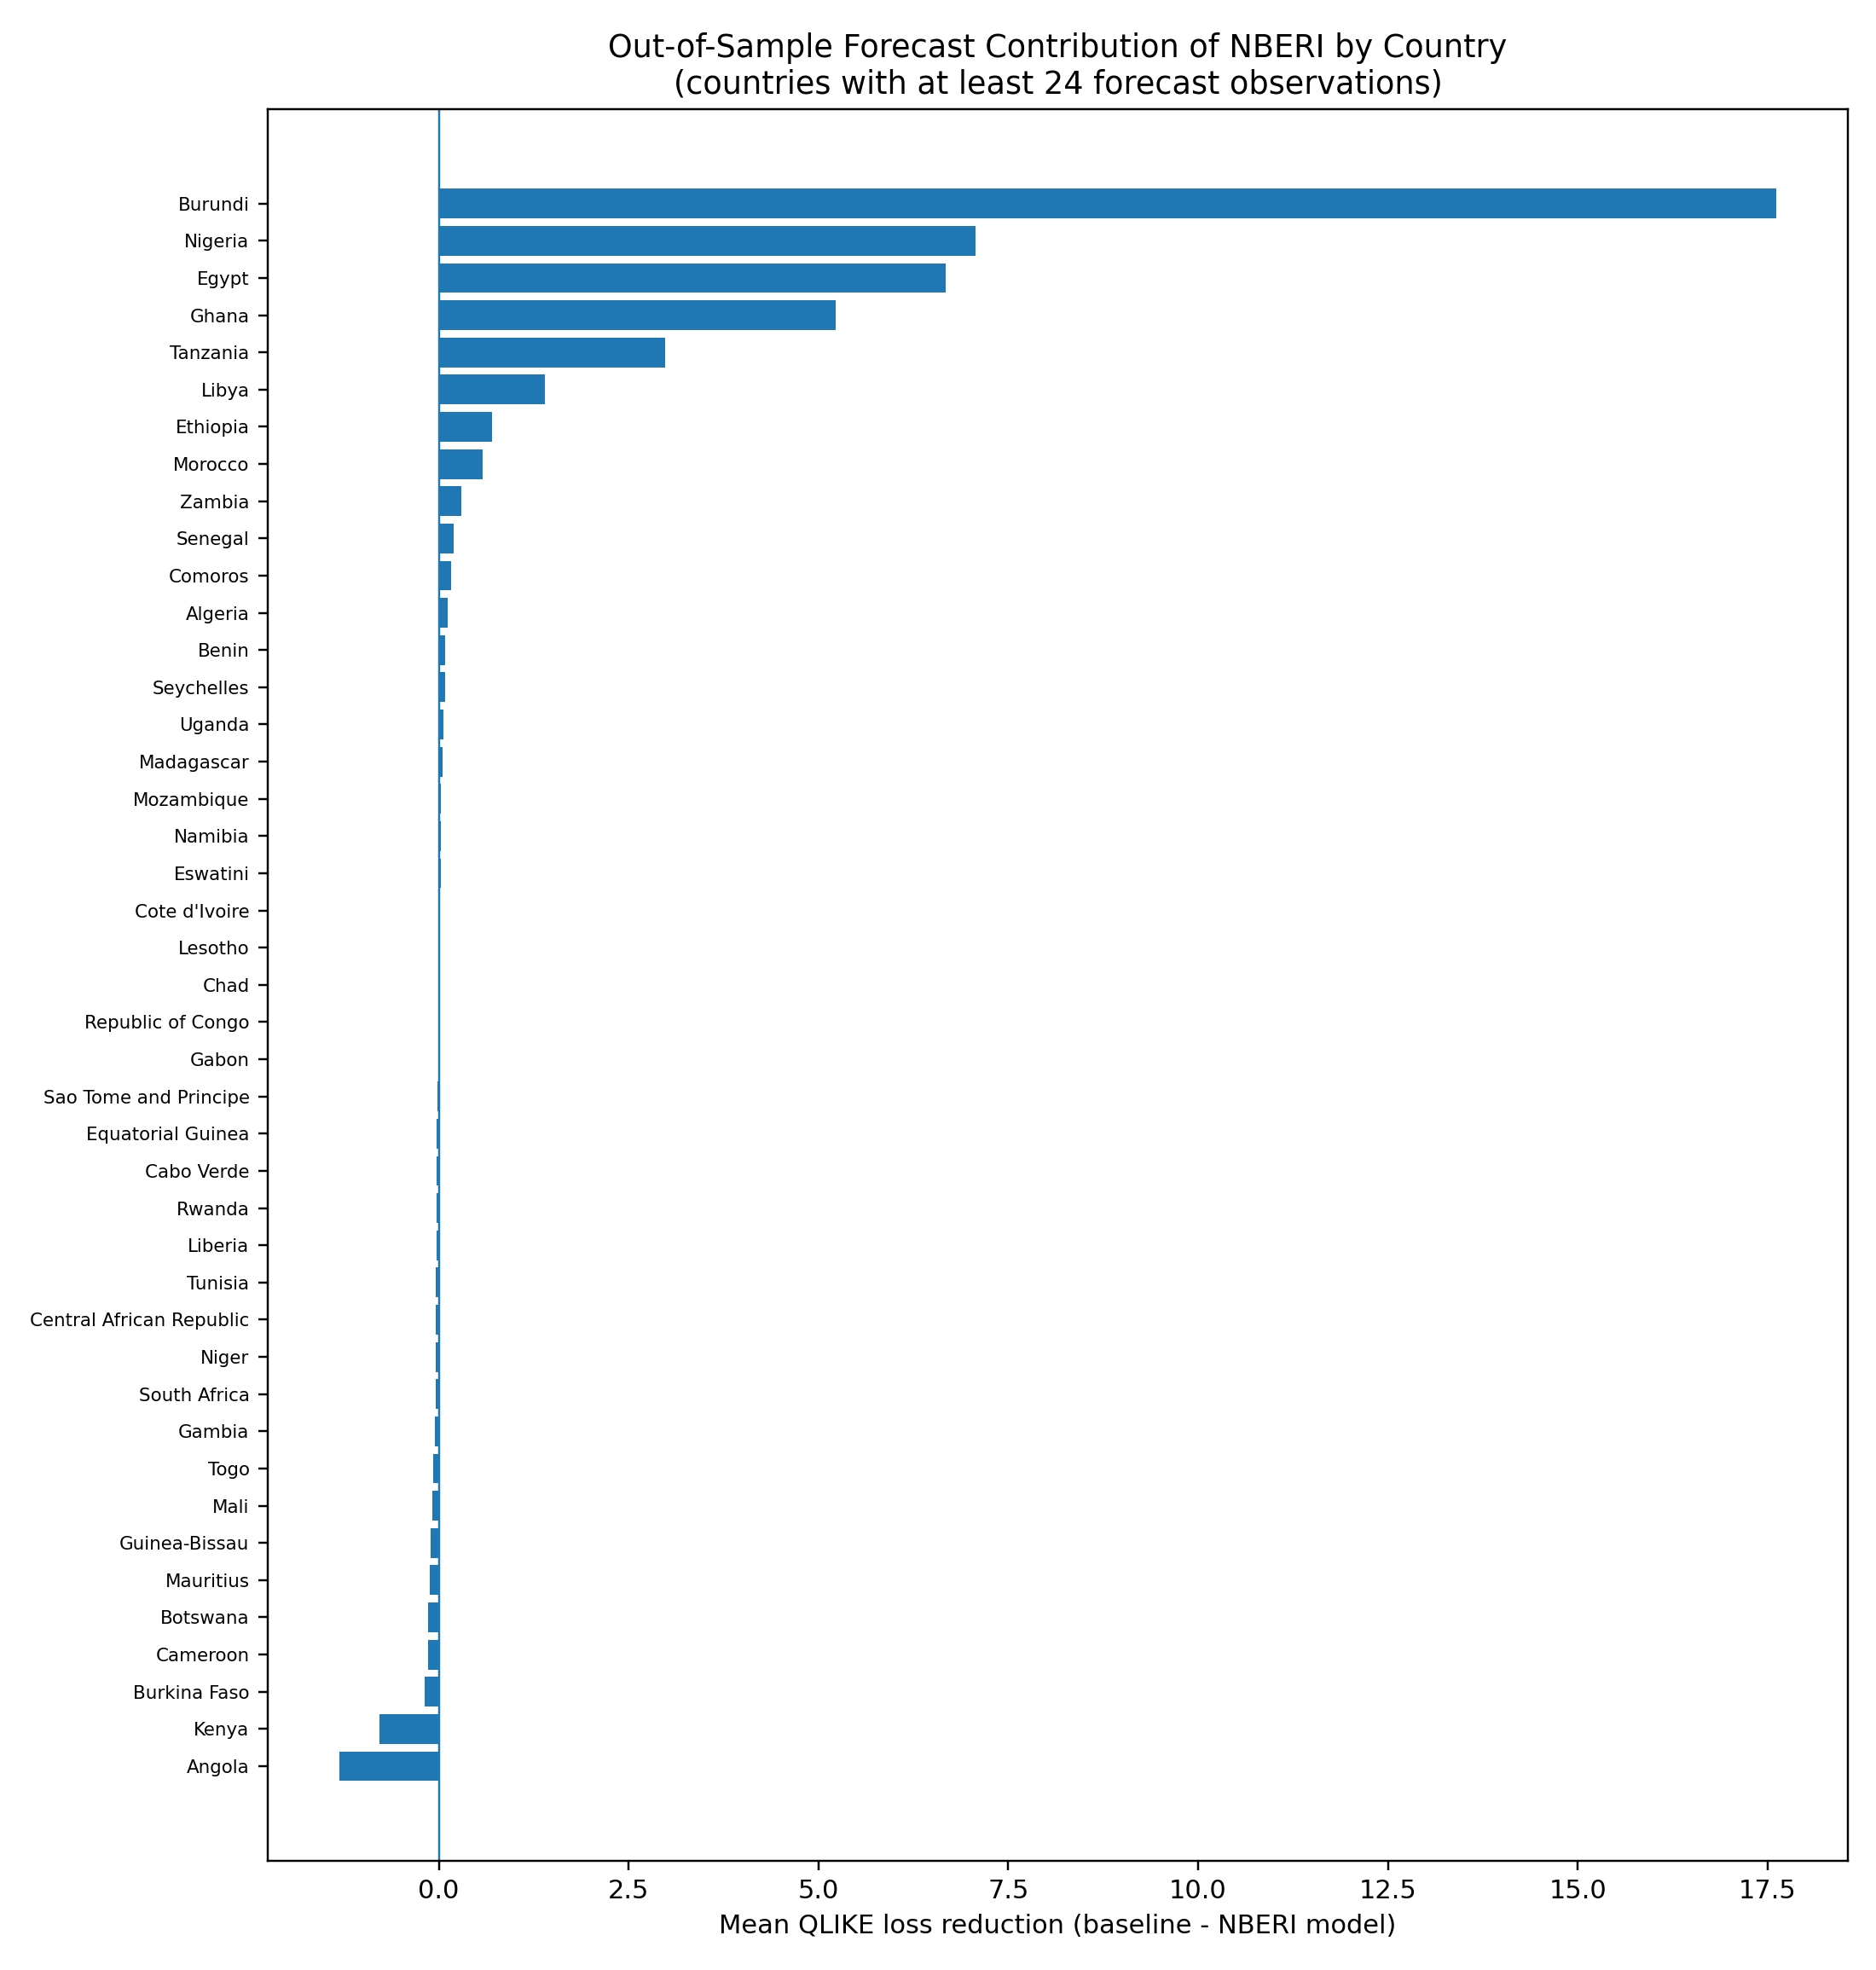
\includegraphics[width=6.1in]{figures/figure7_oos_qlike_continental.png}
\caption{Country-level out-of-sample QLIKE loss reduction from adding NBERI.}
\label{fig:7}
\end{figure}

Out-of-sample evidence supports incremental information, although the
economic magnitude is modest in pooled RMSE. Adding lagged NBERI reduces
pooled RMSE from 2.029 to 2.025, an improvement of approximately 0.20
percent. The Clark-West test rejects equal nested predictive accuracy in
favor of the augmented model (one-sided p = 0.0014). QLIKE also improves
in the pooled sample: the mean monthly loss difference is 1.050, with a
one-sided HAC p-value below 0.001.

The gains are not uniform. Among the 43 countries with at least 24
out-of-sample observations, 23 (53.5 percent) record a positive mean
QLIKE loss reduction. The cross-country distribution includes both
sizable gains and deterioration. This pattern is consistent with NBERI
providing useful incremental information at the continental level while
its forecasting value remains market-dependent.

\subsection{Robustness, persistence, and multiplicity
discipline}\label{robustness-persistence-and-multiplicity-discipline}

The baseline finding is not specific to the log-squared-return
transformation. Replacing the dependent variable with standardized
absolute returns produces an NBERI coefficient of 0.027 (p = 0.010). By
contrast, replacing the lagged NBERI level with its one-month first
difference produces a coefficient of 0.002 (p = 0.803). The predictive
content therefore resides primarily in the sustained risk state rather
than a single-month change in the index.

Country-by-country slope estimates are reported only as diagnostics.
Nine country slopes are nominally significant at the 5 percent level,
but only 1 survives the Benjamini-Hochberg 5 percent
false-discovery-rate correction across 51 countries. The paper
consequently avoids country narratives built on isolated p-values.
Unit-root and stationarity diagnostics are also mixed for NBERI but
considerably stronger for FX returns and the volatility proxy; these
patterns motivate dynamic controls, fixed effects, and
state-versus-change robustness rather than mechanical differencing of
every series.

\clearpage
\subsection{FX-risk/exchange-rate alignment across the top 15
markets}\label{fx-riskexchange-rate-alignment-across-the-top-15-markets}

Table 8. FX-risk pillar and exchange-rate-level alignment, 2015-2025

\begingroup\footnotesize
\begin{longtable}[]{@{}
  >{\raggedright\arraybackslash}p{(\columnwidth - 8\tabcolsep) * \real{0.2000}}
  >{\raggedright\arraybackslash}p{(\columnwidth - 8\tabcolsep) * \real{0.2000}}
  >{\raggedright\arraybackslash}p{(\columnwidth - 8\tabcolsep) * \real{0.2000}}
  >{\raggedright\arraybackslash}p{(\columnwidth - 8\tabcolsep) * \real{0.2000}}
  >{\raggedright\arraybackslash}p{(\columnwidth - 8\tabcolsep) * \real{0.2000}}@{}}
\toprule\noalign{}
\begin{minipage}[b]{\linewidth}\raggedright
\textbf{Country}
\end{minipage} & \begin{minipage}[b]{\linewidth}\raggedright
\textbf{Raw Pearson}
\end{minipage} & \begin{minipage}[b]{\linewidth}\raggedright
\textbf{Spearman}
\end{minipage} & \begin{minipage}[b]{\linewidth}\raggedright
\textbf{Linear-detrended log S}
\end{minipage} & \begin{minipage}[b]{\linewidth}\raggedright
\textbf{Cubic-detrended log S}
\end{minipage} \\
\midrule\noalign{}
\endhead
\bottomrule\noalign{}
\endlastfoot
Zambia & 0.718 & 0.787 & 0.103 & 0.038 \\
Ghana & 0.668 & 0.514 & 0.406 & 0.021 \\
Malawi & 0.649 & 0.467 & 0.358 & 0.225 \\
Tanzania & 0.561 & 0.641 & -0.072 & 0.002 \\
Algeria & 0.549 & 0.562 & 0.542 & 0.477 \\
Burundi & 0.480 & 0.376 & 0.241 & -0.003 \\
Libya & 0.415 & 0.411 & 0.351 & 0.268 \\
Nigeria & 0.322 & 0.150 & 0.439 & 0.338 \\
Tunisia & 0.296 & 0.336 & 0.223 & 0.140 \\
Morocco & 0.285 & 0.237 & 0.327 & 0.283 \\
Liberia & 0.279 & 0.316 & 0.573 & 0.255 \\
Namibia & 0.268 & 0.287 & 0.434 & 0.443 \\
Congo DRC & 0.266 & 0.343 & 0.319 & 0.258 \\
Guinea & 0.263 & 0.382 & -0.062 & -0.180 \\
Benin & 0.247 & 0.325 & 0.256 & 0.289 \\
\end{longtable}
\endgroup

Notes: Raw Pearson correlation is the ranking statistic used to define
the top-15 alignment group. Detrended columns correlate residuals after
removing country-specific linear or cubic time trends from log exchange
rates and the FX-risk pillar. These sensitivity columns diagnose whether
raw level co-movement is dominated by common trending behavior; they are
not used to re-select countries.

\begin{figure}[!htbp]
\centering
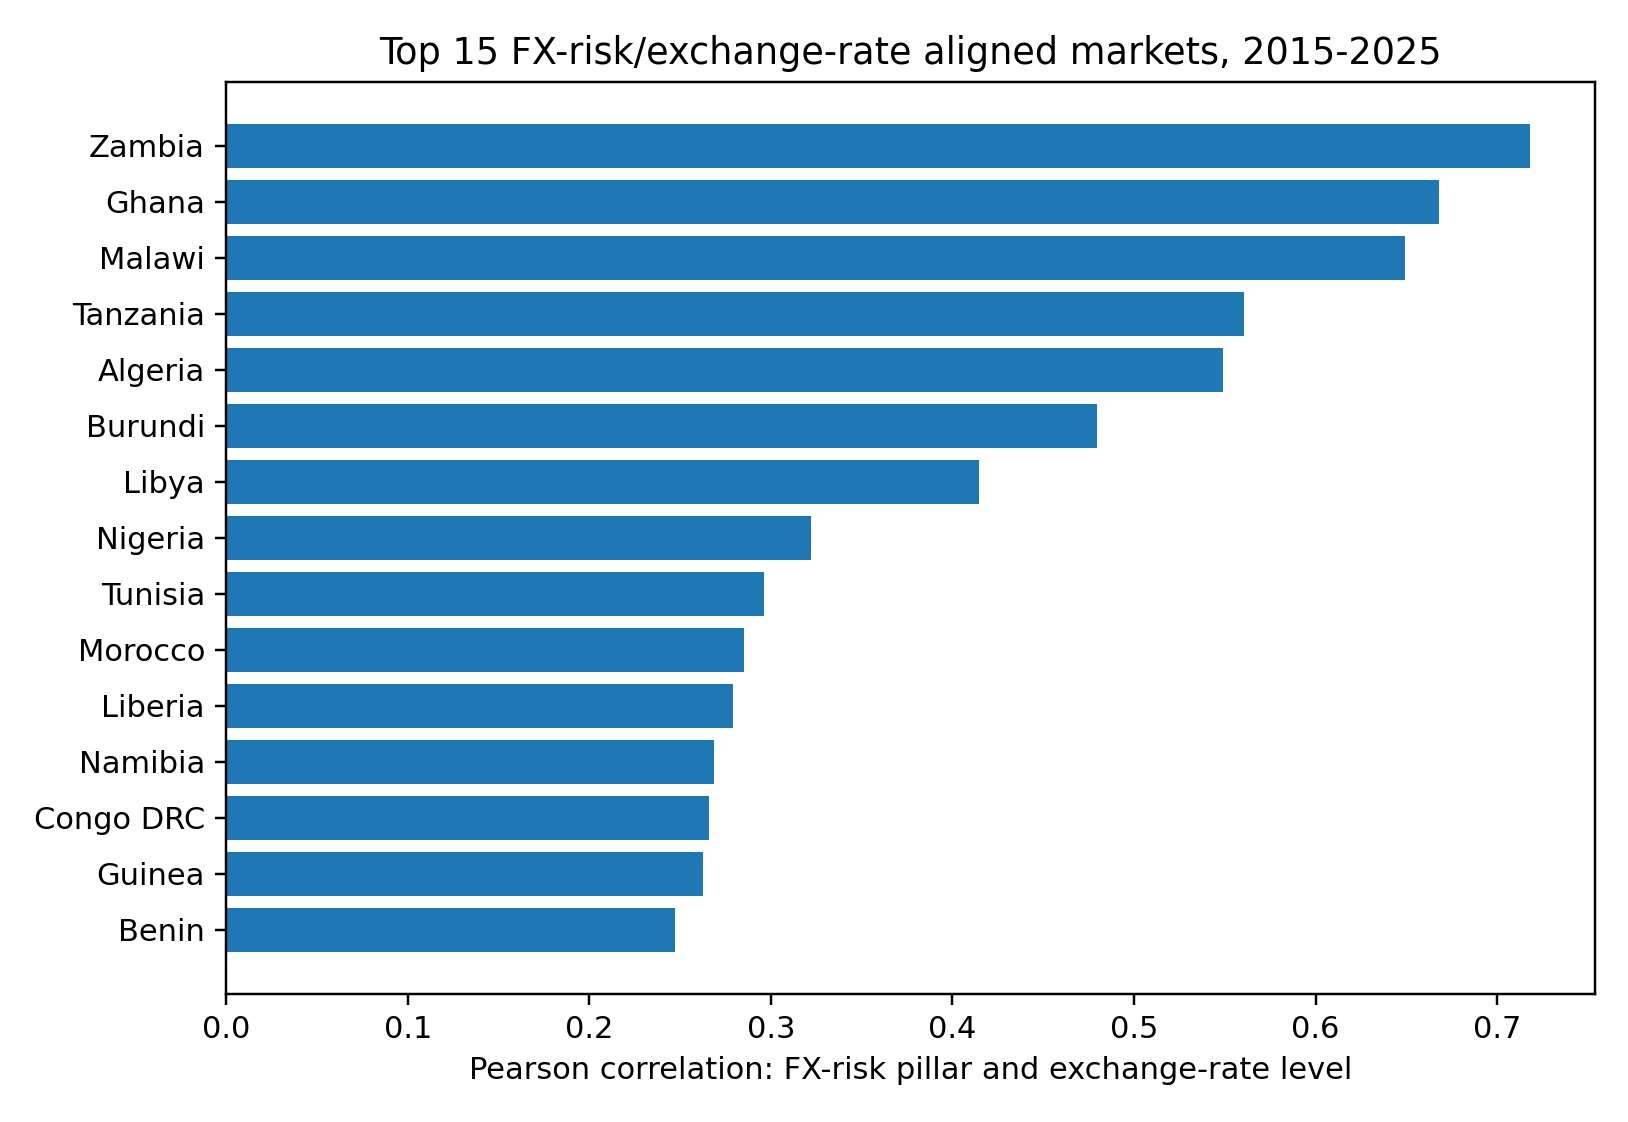
\includegraphics[width=6.3in]{figures/figure8_alignment_top15.png}
\caption{Top 15 FX-risk/exchange-rate aligned markets.}
\label{fig:8}
\end{figure}

The alignment ranking is economically heterogeneous rather than a simple
proxy for trend. Raw correlations range from 0.718 in Zambia to 0.247 in
Benin. Rank correlations remain positive for all 15 markets and exceed
0.40 in several cases, while detrended correlations are strong in
Algeria, Nigeria, Namibia, Liberia, Ghana, Malawi, and Libya but much
weaker in Zambia, Tanzania, and Guinea. This pattern is precisely why
the level correlation is treated as a screening statistic rather than an
identifying variable: it identifies markets in which the news-risk state
and the observed FX state co-move strongly in levels, but the mechanism
behind that co-movement differs across countries.

\subsection{Does alignment identify stronger risk-to-volatility
transmission?}\label{does-alignment-identify-stronger-risk-to-volatility-transmission}

Table 9. Full-sample tests of alignment heterogeneity

\begingroup\footnotesize
\begin{longtable}[]{@{}
  >{\raggedright\arraybackslash}p{(\columnwidth - 6\tabcolsep) * \real{0.2500}}
  >{\raggedright\arraybackslash}p{(\columnwidth - 6\tabcolsep) * \real{0.2500}}
  >{\raggedright\arraybackslash}p{(\columnwidth - 6\tabcolsep) * \real{0.2500}}
  >{\raggedright\arraybackslash}p{(\columnwidth - 6\tabcolsep) * \real{0.2500}}@{}}
\toprule\noalign{}
\begin{minipage}[b]{\linewidth}\raggedright
\textbf{Test}
\end{minipage} & \begin{minipage}[b]{\linewidth}\raggedright
\textbf{Estimate}
\end{minipage} & \begin{minipage}[b]{\linewidth}\raggedright
\textbf{SE / benchmark}
\end{minipage} & \begin{minipage}[b]{\linewidth}\raggedright
\textbf{p-value}
\end{minipage} \\
\midrule\noalign{}
\endhead
\bottomrule\noalign{}
\endlastfoot
FE: remaining eligible slope & 0.017 & 0.012 & 0.147 \\
FE: selected-15 incremental slope & 0.046 & 0.026 & 0.074 \\
FE: selected-15 total slope & 0.063 & 0.023 & 0.007 \\
LP h=1: remaining eligible slope & 0.029 & 0.013 & 0.032 \\
LP h=1: selected-15 incremental slope & 0.072 & 0.030 & 0.019 \\
LP h=1: selected-15 total slope & 0.100 & 0.025 & 0.000 \\
Continuous NBERI x alignment interaction & 0.012 & 0.015 & 0.412 \\
Random-subset benchmark: selected total slope & 0.061 & 94.4th
percentile & 0.057 \\
\end{longtable}
\endgroup

Notes: Fixed-effects and local-projection interaction models are
estimated in the full eligible-country panel with country and
calendar-time effects and the same dynamic controls used in the
benchmark. The random-subset benchmark compares the selected group with
1,000 draws of 15 eligible countries and reports an empirical one-sided
probability.

\begin{figure}[!htbp]
\centering
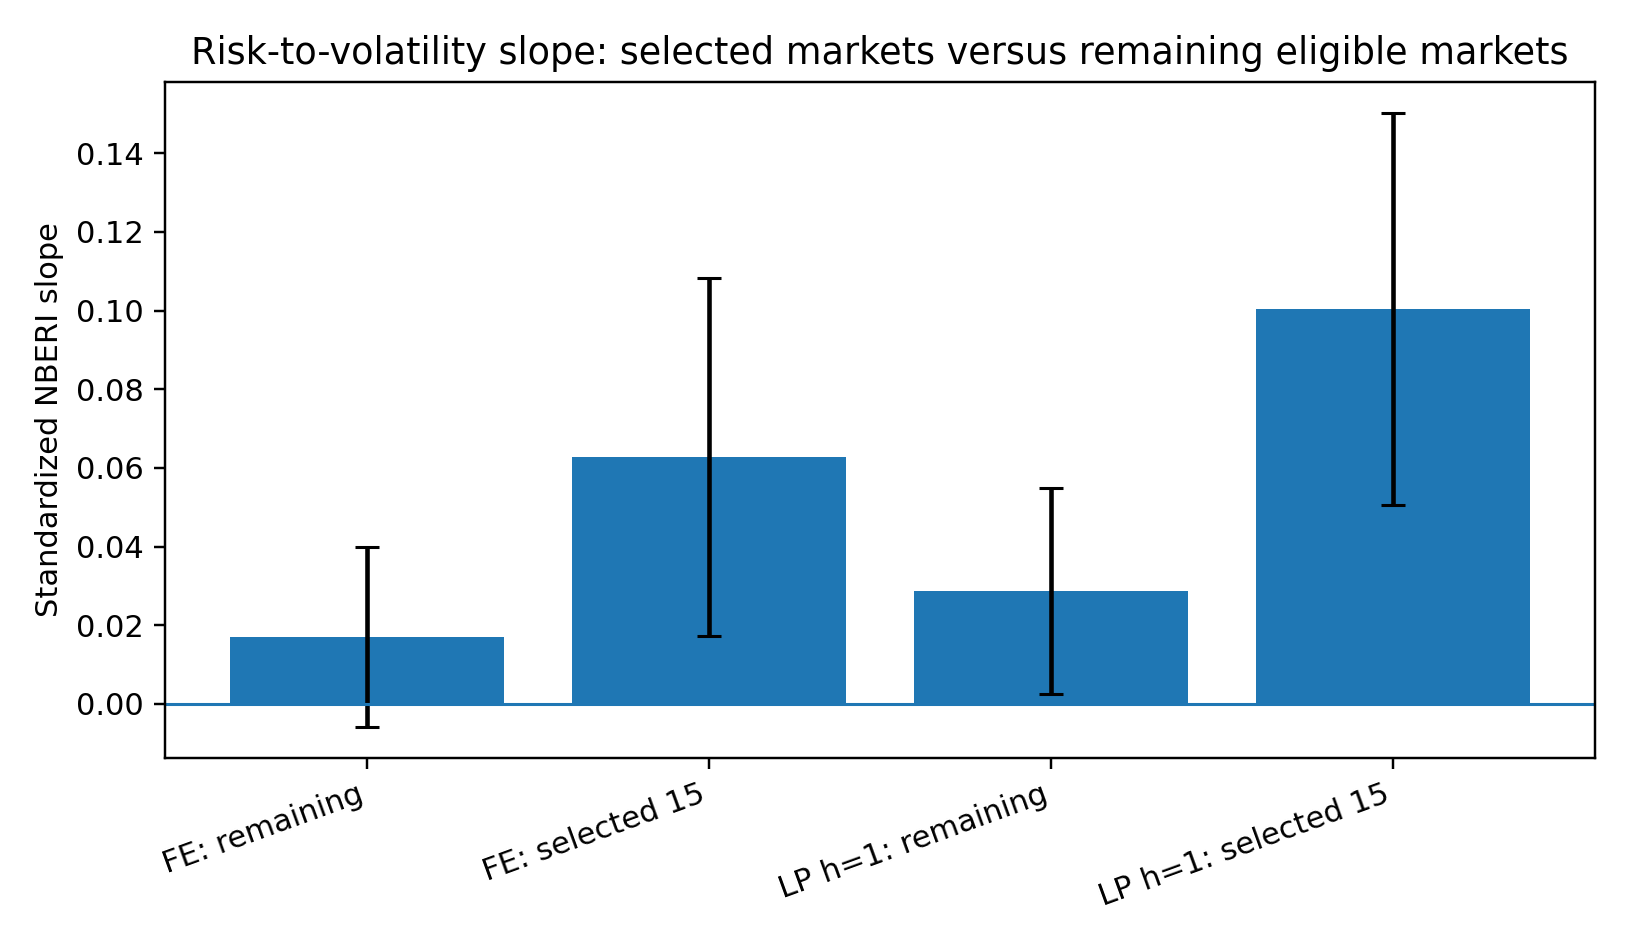
\includegraphics[width=6.2in]{figures/figure9_alignment_group_slopes.png}
\caption{Risk-to-volatility slopes in aligned and remaining eligible markets.}
\label{fig:9}
\end{figure}

The group comparison provides the formal evidence that the alignment
screen is associated with stronger transmission. In the remaining
eligible markets, the lagged-NBERI coefficient is 0.017 (p = 0.147). The
selected-15 total slope is 0.063 (p = 0.007), with an incremental
selected-group effect of 0.046 (p = 0.074). The horizon-1 result is
sharper: the remaining-market slope is 0.029 (p = 0.032), the
selected-group slope is 0.100 (p \textless{} 0.001), and the
selected-group increment is 0.072 (p = 0.019). The selected-group
fixed-effects slope lies near the 94th percentile of 1,000 random
15-country subsets, with a one-sided empirical probability of
approximately 0.057. This is suggestive rather than decisive permutation
evidence, but it shows that the top-15 result is not typical of an
arbitrary 15-country draw.

The continuous interaction between NBERI and the country-level alignment
coefficient is positive but insignificant (0.012, p = 0.412). Alignment
therefore does not act as a linear dose-response moderator. The evidence
is better described as a grouped market-state distinction: the
highest-alignment markets collectively display stronger short-horizon
transmission, but a larger raw level correlation does not mechanically
imply a proportionally larger volatility coefficient.

\subsection{Dynamic and forecast evidence in the aligned-market
subsample}\label{dynamic-and-forecast-evidence-in-the-aligned-market-subsample}

Table 10. Dynamic and forecast evidence in the 15 aligned markets

\begingroup\footnotesize
\begin{longtable}[]{@{}
  >{\raggedright\arraybackslash}p{(\columnwidth - 6\tabcolsep) * \real{0.2500}}
  >{\raggedright\arraybackslash}p{(\columnwidth - 6\tabcolsep) * \real{0.2500}}
  >{\raggedright\arraybackslash}p{(\columnwidth - 6\tabcolsep) * \real{0.2500}}
  >{\raggedright\arraybackslash}p{(\columnwidth - 6\tabcolsep) * \real{0.2500}}@{}}
\toprule\noalign{}
\begin{minipage}[b]{\linewidth}\raggedright
\textbf{Result}
\end{minipage} & \begin{minipage}[b]{\linewidth}\raggedright
\textbf{Estimate}
\end{minipage} & \begin{minipage}[b]{\linewidth}\raggedright
\textbf{SE / interval}
\end{minipage} & \begin{minipage}[b]{\linewidth}\raggedright
\textbf{p-value}
\end{minipage} \\
\midrule\noalign{}
\endhead
\bottomrule\noalign{}
\endlastfoot
Two-way FE: lagged NBERI & 0.068 & 0.027 & 0.013 \\
PVAR volatility equation: lagged NBERI & 0.068 & 0.027 & 0.013 \\
Generalized IRF, h=1 & 0.099 & 95\% CI {[}0.054, 0.131{]} & \\
12-month FEVD share from NBERI & 3.39\% & & \\
Local projection, h=1 & 0.121 & 0.032 & 0.0001 \\
Absolute-return robustness & 0.066 & 0.029 & 0.023 \\
First-difference NBERI robustness & -0.025 & 0.031 & 0.406 \\
Forecast RMSE improvement & 0.89\% & & \\
Forecast QLIKE improvement & 2.85\% & & \\
Clark-West nested test & 0.123 & & p = 0.0005 \\
QLIKE loss-difference test & 1.589 & & p = 0.123 \\
\end{longtable}
\endgroup

\begin{figure}[!htbp]
\centering
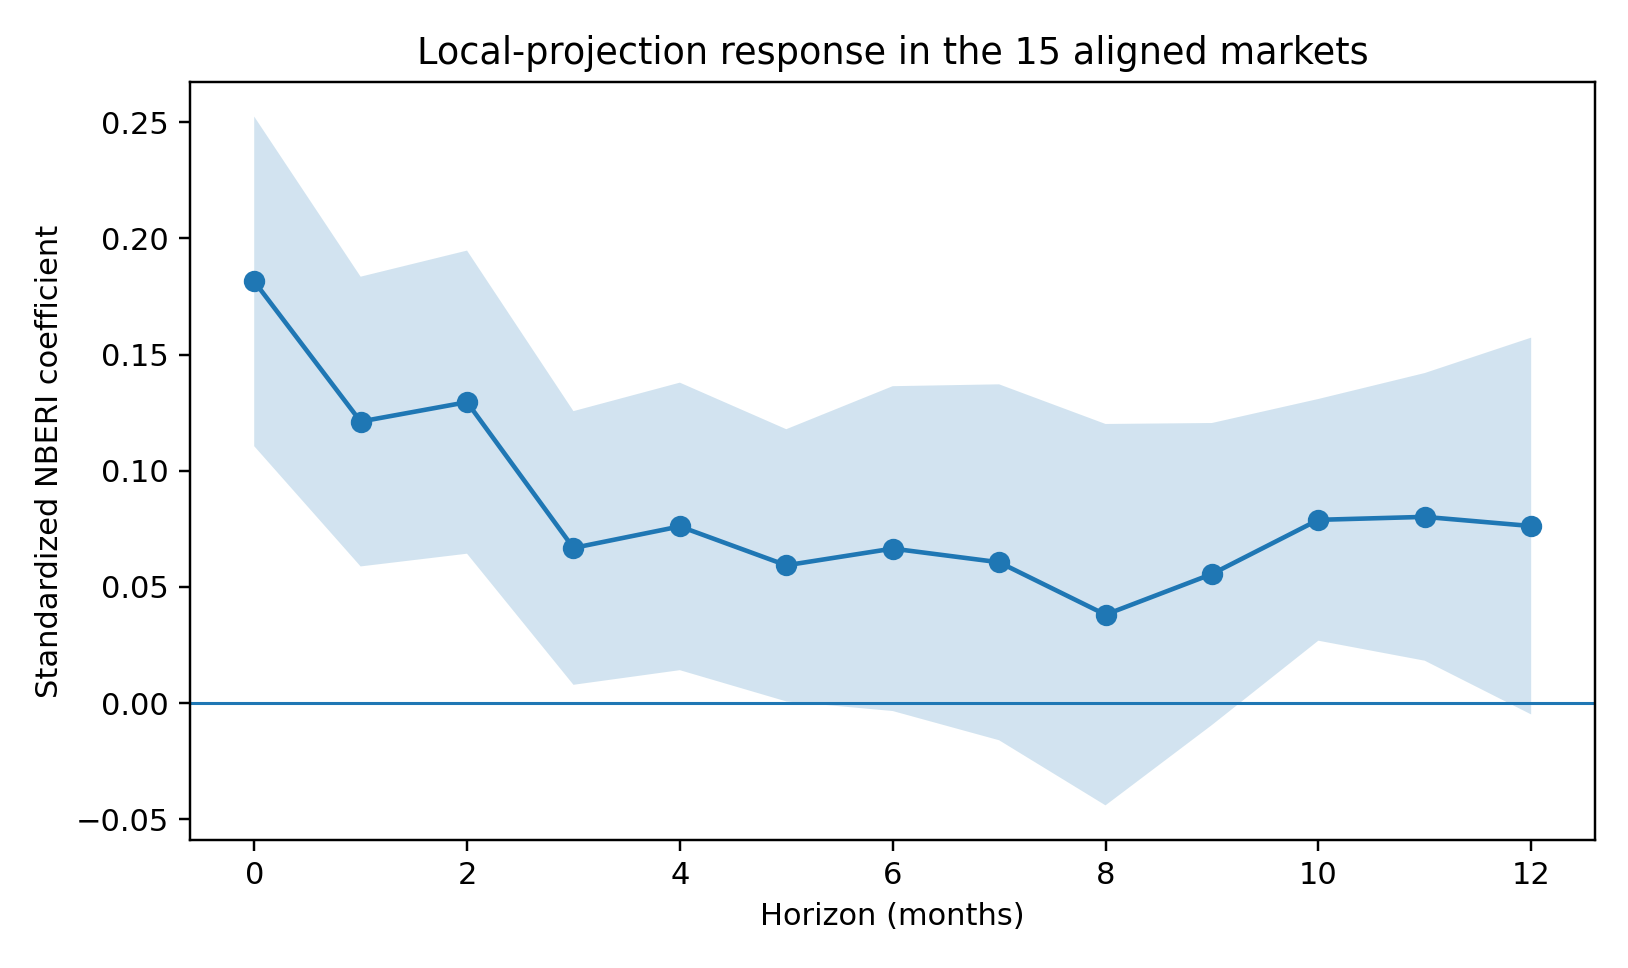
\includegraphics[width=6.2in]{figures/figure10_local_projection_aligned15.png}
\caption{Local-projection response in the 15 aligned markets.}
\label{fig:10}
\end{figure}

The aligned-market subsample strengthens the dynamic signal without
changing its interpretation. The fixed-effects coefficient is 0.068 (p =
0.013), more than twice the continental coefficient. The PVAR returns
the same one-step coefficient and remains dynamically stable, with a
maximum companion-root modulus of 0.483. A one-standard-deviation NBERI
innovation generates a generalized volatility response of 0.099 at
horizon 1, with a 95 percent country-block bootstrap interval of 0.054
to 0.131, and 0.056 at horizon 2. NBERI accounts for 3.39 percent of the
12-month volatility forecast-error variance, compared with 1.05 percent
in the continental system.

Local projections show a broad near-term response: the h=1 coefficient
is 0.121 (p \textless{} 0.001), h=2 is 0.130 (p \textless{} 0.001), and
the response remains positive through several subsequent horizons. The
absolute-return specification is also positive (0.066, p = 0.023),
whereas the first difference of NBERI is insignificant (-0.025, p =
0.406). As in the continental results, the information appears to reside
in a persistent risk state rather than a one-month jump in the index.

\subsection{Country-level GARCH-family evidence and out-of-sample
gains}\label{country-level-garch-family-evidence-and-out-of-sample-gains}

Table 11. Profile-likelihood GARCH-family results surviving
within-family FDR correction

\begingroup\footnotesize
\begin{longtable}[]{@{}
  >{\raggedright\arraybackslash}p{(\columnwidth - 12\tabcolsep) * \real{0.1429}}
  >{\raggedright\arraybackslash}p{(\columnwidth - 12\tabcolsep) * \real{0.1429}}
  >{\raggedright\arraybackslash}p{(\columnwidth - 12\tabcolsep) * \real{0.1429}}
  >{\raggedright\arraybackslash}p{(\columnwidth - 12\tabcolsep) * \real{0.1429}}
  >{\raggedright\arraybackslash}p{(\columnwidth - 12\tabcolsep) * \real{0.1429}}
  >{\raggedright\arraybackslash}p{(\columnwidth - 12\tabcolsep) * \real{0.1429}}
  >{\raggedright\arraybackslash}p{(\columnwidth - 12\tabcolsep) * \real{0.1429}}@{}}
\toprule\noalign{}
\begin{minipage}[b]{\linewidth}\raggedright
\textbf{Country}
\end{minipage} & \begin{minipage}[b]{\linewidth}\raggedright
\textbf{Model}
\end{minipage} & \begin{minipage}[b]{\linewidth}\raggedright
\textbf{delta}
\end{minipage} & \begin{minipage}[b]{\linewidth}\raggedright
\textbf{LR p}
\end{minipage} & \begin{minipage}[b]{\linewidth}\raggedright
\textbf{BH q}
\end{minipage} & \begin{minipage}[b]{\linewidth}\raggedright
\textbf{LB(5) sq. p}
\end{minipage} & \begin{minipage}[b]{\linewidth}\raggedright
\textbf{ARCH-LM(5) p}
\end{minipage} \\
\midrule\noalign{}
\endhead
\bottomrule\noalign{}
\endlastfoot
Ghana & EGARCH-X & 0.766 & 0.0002 & 0.0036 & 0.044 & 0.078 \\
Libya & GARCH-X & 0.645 & 0.0005 & 0.0074 & 1.000 & 1.000 \\
\end{longtable}
\endgroup

Notes: Reported rows are the only country-family X effects that survive
Benjamini-Hochberg q \textless{} 0.10 after profile-likelihood
refinement of the NBERI variance coefficient. Forty-five X models are
tested in total: GARCH-X, EGARCH-X, and GJR/TGARCH-X for each of 15
countries. Full results are reported in Appendix H.

\begin{figure}[!htbp]
\centering
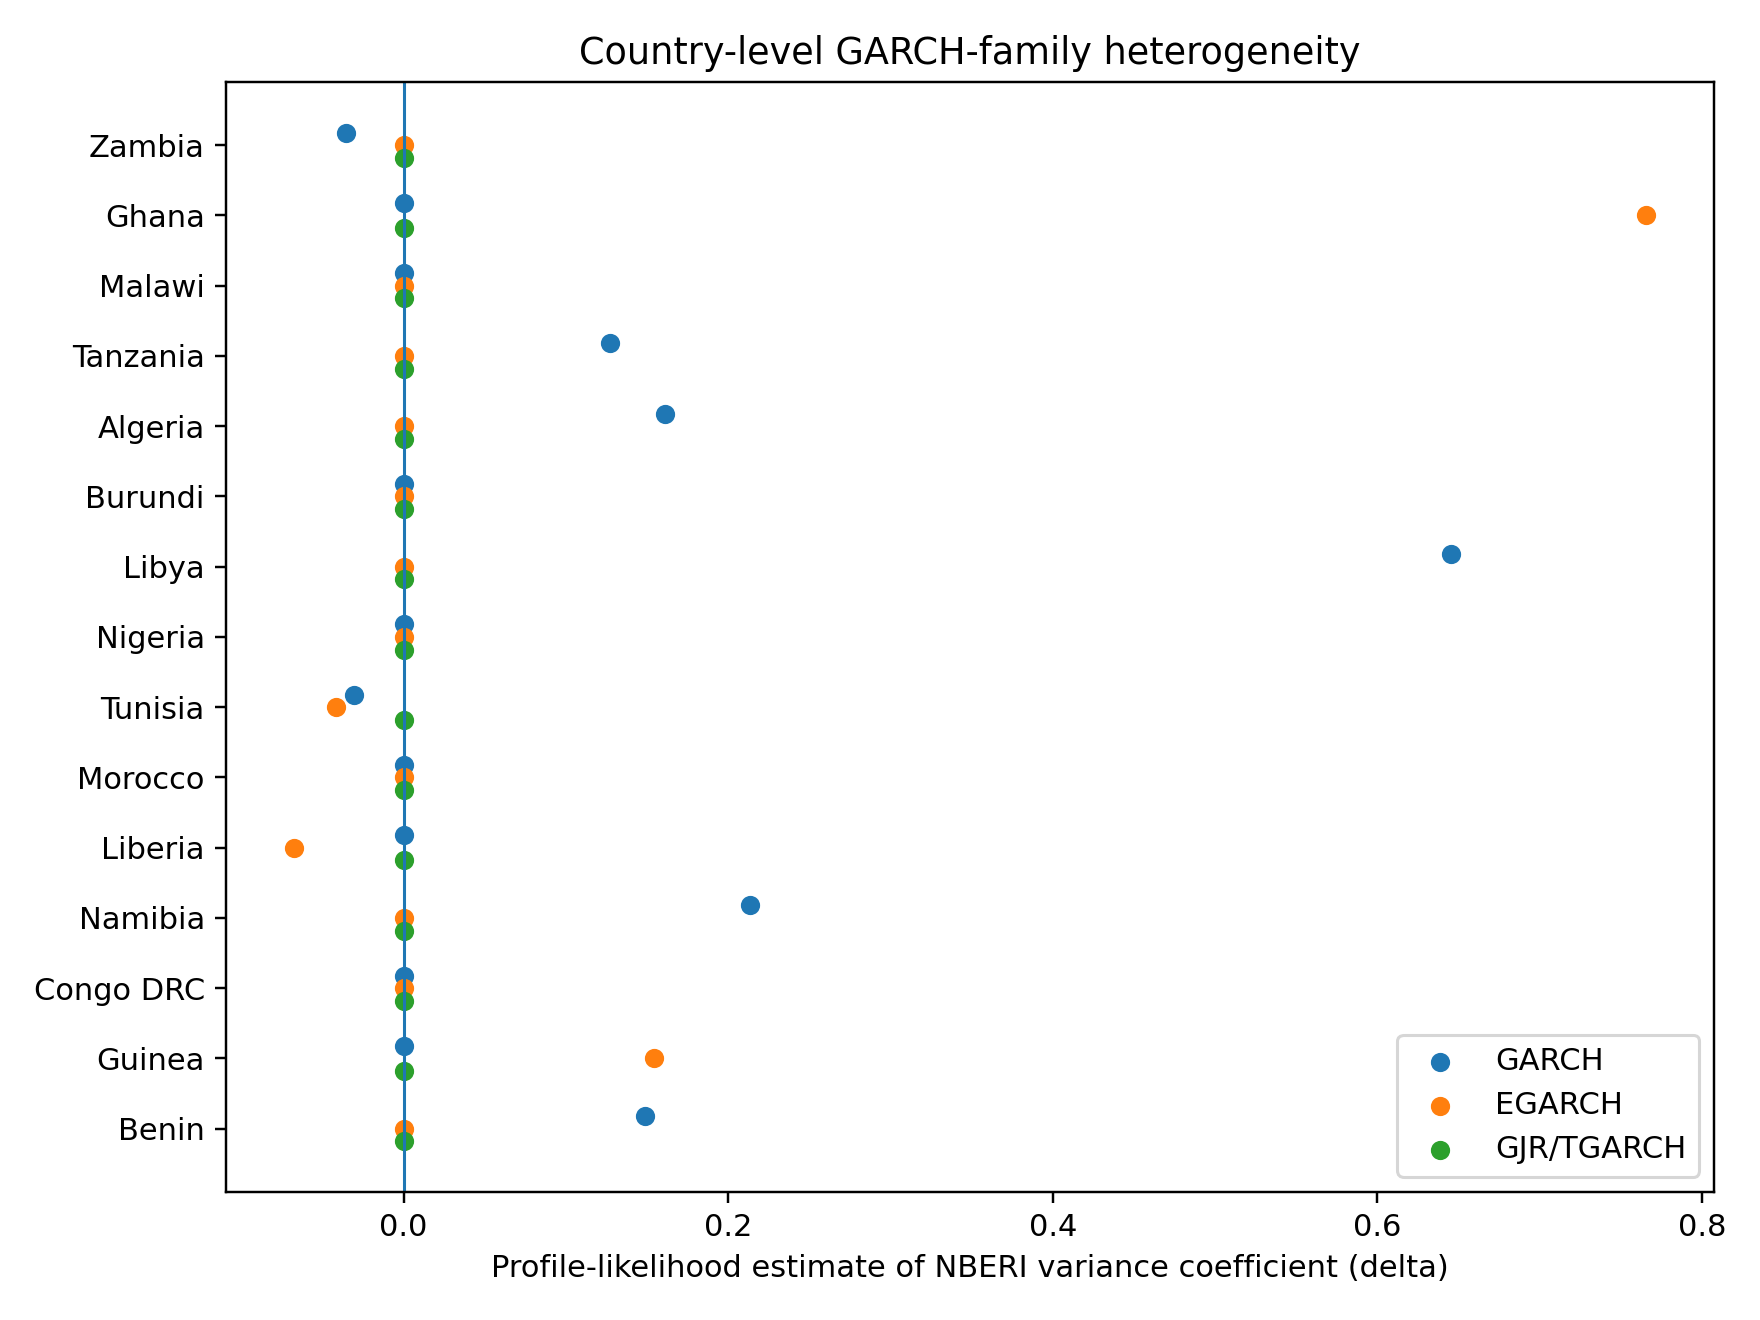
\includegraphics[width=6.4in]{figures/figure11_profile_garch.png}
\caption{Profile-likelihood NBERI variance coefficients across the 15-country GARCH family.}
\label{fig:11}
\end{figure}

The profile-likelihood exercise sharply disciplines the country-level
GARCH evidence. Only two effects survive within-family false-discovery
control: Ghana under EGARCH-X (delta = 0.766; LR p = 0.00024; q =
0.0036) and Libya under GARCH-X (delta = 0.645; LR p = 0.00050; q =
0.0074). Libya passes the squared-residual and ARCH diagnostics
comfortably. Ghana\textquotesingle s ARCH-LM diagnostic is acceptable at
conventional levels, although the Ljung-Box test on squared standardized
residuals is borderline at p = 0.044; the Ghana result is therefore
interpreted with additional caution. The remaining 43 country-family X
tests do not survive q \textless{} 0.10 after the profile-likelihood
refinement.\footnote{The false-discovery-rate adjustment is applied within model family across the 15 aligned countries. This is deliberately stricter than highlighting isolated nominal p-values from dozens of country-model combinations.} This result is more informative than a large collection of
nominal country p-values: it shows that conditional-variance
transmission exists in specific markets but is not a general feature of
the aligned sample.

\begin{figure}[!htbp]
\centering
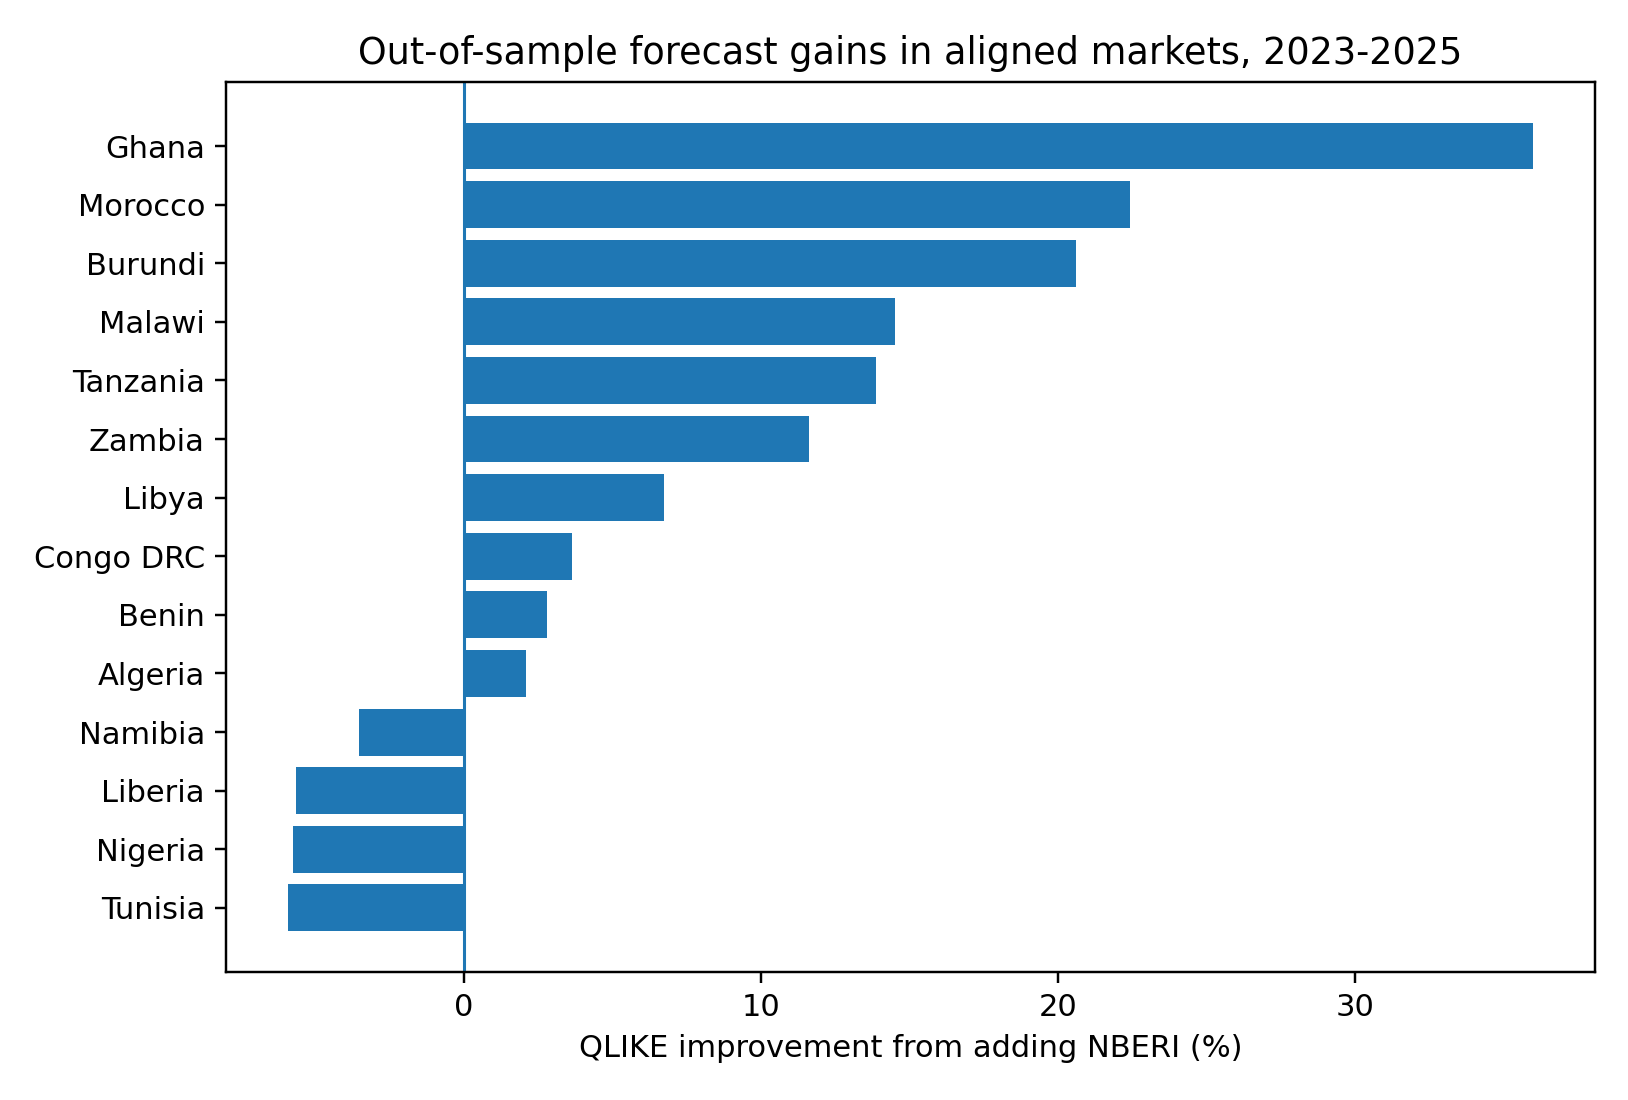
\includegraphics[width=6.25in]{figures/figure12_oos_qlike_aligned15.png}
\caption{Country-level QLIKE improvement from adding NBERI in the aligned-market forecast experiment.}
\label{fig:12}
\end{figure}

The forecast horse race adds a genuine prediction test. Across the
aligned markets, adding lagged NBERI lowers pooled RMSE by 0.89 percent,
from 2.254 to 2.234, and the Clark-West test favors the augmented model
(p = 0.0005). Mean QLIKE falls by 2.85 percent, although the HAC test of
the pooled QLIKE loss difference is not significant at conventional
levels (p = 0.123). The country distribution is heterogeneous: Ghana
records the largest QLIKE improvement, followed by Morocco and Burundi,
while several countries show small deteriorations. The forecast evidence
therefore supports incremental predictive content without implying
uniform country-level dominance.

\section{Discussion, Conclusion, and Limitations}\label{discussion}

\subsection{Continental leading information and the boundary of the
claim}\label{continental-leading-information-and-the-boundary-of-the-claim}

The continental evidence establishes the baseline result: NBERI contains
leading information about subsequent monthly exchange-rate instability.
The coefficient survives market-history controls, inflation, country
effects, common time shocks, and the collapse of repeated currency-union
paths. PVARs, generalized responses, local projections, absolute-return
robustness, and out-of-sample tests all point in the same direction. The
size is economically modest, which is appropriate for an incremental
information variable rather than a stand-alone market model.

The pooled GARCH-X null remains an important boundary. The common
monthly variance recursion is extremely persistent and does not admit a
statistically meaningful continent-wide NBERI variance coefficient. The
new country-family exercise does not overturn that result; it explains
it. After profile-likelihood refinement and multiplicity control, only
Ghana and Libya exhibit robust family-specific X effects. The absence of
a universal variance parameter is therefore not evidence that NBERI
lacks information. It indicates that the information enters market
dynamics through heterogeneous channels rather than one common GARCH
mechanism.

\subsection{Market alignment as an organizing device for
heterogeneity}\label{market-alignment-as-an-organizing-device-for-heterogeneity}

The market-alignment extension provides the paper\textquotesingle s main
heterogeneity result. The top-15 aligned markets have a larger total
fixed-effects slope than the remaining eligible countries and a
significantly larger horizon-1 local-projection response. The
selected-group coefficient also lies near the 94th percentile of random
15-country subsets. At the same time, the continuous alignment
interaction is insignificant, so the raw correlation should not be
interpreted as a structural moderator measured on a cardinal scale. The
useful insight is categorical and empirical: markets in which FX-risk
narratives and the observed exchange-rate state are most tightly
synchronized, as a group, transmit the news-risk state into subsequent
volatility more strongly.

\subsection{Why the GARCH-family and forecast results
matter}\label{why-the-garch-family-and-forecast-results-matter}

The combined evidence separates three objects that are often conflated:
information, conditional variance, and forecasting value. NBERI is
informative in the panel and local-projection sense;
conditional-variance effects are concentrated in a small number of
countries; and out-of-sample gains are positive on average but uneven
across markets and loss functions. This distinction is operationally
useful. A surveillance system can treat NBERI as a state variable that
enriches the information set without assuming that it enters every
currency\textquotesingle s variance equation or improves every forecast
origin.

\subsection{Contribution to empirical FX-risk
measurement}\label{contribution-to-empirical-fx-risk-measurement}

The paper contributes an empirical architecture for evaluating
text-based market-risk measures rather than merely documenting
correlation. The architecture begins with a broad panel, separates news
risk from market outcomes, tests effective currency-market dependence,
distinguishes predictive regressions from conditional-variance
recursions, traces dynamic propagation, imposes real-time forecast
evaluation, and then uses an alignment screen only as a disciplined
heterogeneity extension. The resulting conclusion is stronger because it
is narrower: NBERI is a leading information state with economically
meaningful market heterogeneity, not a universal structural volatility
factor.

\subsection{Conclusion}

This paper evaluates a news-based exchange-rate risk measure across the
broadest African sample supported by the supplied monthly data and adds
a new market-alignment framework for understanding why the signal is
stronger in some currency markets than others. Of 54 source countries,
51 pass pre-specified coverage and variation screens. The design keeps
the news measure separate from market outcomes, adjusts inference for
serial and cross-sectional dependence, collapses shared-currency paths,
and combines panel prediction, dynamic propagation, conditional-variance
models, and real-time forecast evaluation in one framework.

The continental result is a positive but moderate leading relationship:
a one-standard-deviation increase in lagged NBERI predicts approximately
0.03 standard deviations more next-month FX volatility after controls,
and the relationship survives the 36-cluster currency-market robustness.
The alignment extension adds a second result. In the top 15
FX-risk/exchange-rate aligned markets, the fixed-effects coefficient is
0.068 (p = 0.013), the horizon-1 local-projection response is 0.121 (p
\textless{} 0.001), and NBERI explains 3.39 percent of the 12-month
volatility forecast-error variance. Full-sample interaction tests show
that the aligned group has a significantly larger horizon-1 slope than
the remaining eligible markets.

Out-of-sample performance is consistent with incremental rather than
dominant predictive value. In the aligned markets, NBERI lowers pooled
RMSE by 0.89 percent and passes the Clark-West nested forecast test,
while the pooled QLIKE improvement is positive but not statistically
decisive under the HAC loss-difference test. The country-level GARCH
family provides an equally important boundary: after profile-likelihood
refinement and false-discovery correction, robust NBERI variance effects
survive only in Ghana and Libya. The common pooled GARCH-X null and the
selective country-family evidence are therefore mutually consistent.

The paper\textquotesingle s novel contribution is the separation of
broad informational content from market-specific volatility
transmission. News-based FX risk contains measurable leading information
across the continent, but the strength and mechanism of that information
depend on market context. The market-alignment layer identifies a group
with stronger short-horizon transmission without converting a
descriptive level correlation into a causal claim. For surveillance,
this implies that text-based FX-risk measures are most useful as
disciplined additions to the market information set, with
country-specific model validation determining when they should enter
conditional-variance or forecasting systems.

\subsection{Limitations}

The main limitation is data frequency. Monthly exchange rates cannot
recover intramonth quadratic variation, so the panel outcome is a
monthly volatility proxy and the GARCH-family models have relatively
short time series. This is why the panel, dynamic, and forecast evidence
carries more weight than any single country-level variance recursion.
Higher-frequency exchange-rate data would permit sharper GARCH-X,
EGARCH-X, and threshold-volatility tests.

A second limitation concerns the market-alignment screen. Exchange-rate
levels can be persistent or trending, and a contemporaneous level
correlation is not an identification strategy. The paper therefore
treats the top-15 ranking as descriptive, reports rank and detrended
sensitivity measures, performs full-sample interaction tests, and
compares the selected group with random 15-country subsets. These checks
strengthen the heterogeneity interpretation but do not make the
alignment coefficient causal.

Finally, NBERI is observational and the 2023-2025 forecast evaluation
window is short relative to the full estimation period. Lagging the
index, fixed effects, reverse PVAR paths, state-versus-change
robustness, profile-likelihood volatility tests, multiplicity control,
and genuine out-of-sample evaluation narrow several alternative
explanations but do not identify an exogenous structural shock. The
paper therefore maintains predictive language and treats
country-specific mechanisms as hypotheses for future work with
higher-frequency prices and richer institutional covariates.

\phantomsection\addcontentsline{toc}{section}{References}
\begin{thebibliography}{99}
\setlength{\itemsep}{0.35em}

\bibitem[Abrigo and Love(2016)]{abrigo2016}
Abrigo, M. R. M., \& Love, I. (2016). Estimation of panel vector autoregression in Stata. \textit{Stata Journal}, 16(3), 778--804.

\bibitem[Akosah(2014)]{akosah2014}
Akosah, N. K. (2014). Volatility and asymmetry of the USD/GHS exchange rate: Monetary policy implications in Ghana. \textit{Ghanaian Journal of Economics}, 2(1).

\bibitem[Andersen et~al.(2003)]{andersen2003}
Andersen, T. G., Bollerslev, T., Diebold, F. X., \& Vega, C. (2003). Micro effects of macro announcements: Real-time price discovery in foreign exchange. \textit{American Economic Review}, 93(1), 38--62.

\bibitem[Baker et~al.(2016)]{baker2016}
Baker, S. R., Bloom, N., \& Davis, S. J. (2016). Measuring economic policy uncertainty. \textit{Quarterly Journal of Economics}, 131(4), 1593--1636.

\bibitem[Benjamini and Hochberg(1995)]{benjamini1995}
Benjamini, Y., \& Hochberg, Y. (1995). Controlling the false discovery rate: A practical and powerful approach to multiple testing. \textit{Journal of the Royal Statistical Society: Series B}, 57(1), 289--300.

\bibitem[Bollerslev(1986)]{bollerslev1986}
Bollerslev, T. (1986). Generalized autoregressive conditional heteroskedasticity. \textit{Journal of Econometrics}, 31(3), 307--327.

\bibitem[Caldara and Iacoviello(2022)]{caldara2022}
Caldara, D., \& Iacoviello, M. (2022). Measuring geopolitical risk. \textit{American Economic Review}, 112(4), 1194--1225.

\bibitem[Cermeño and Grier(2006)]{cermeno2006}
Cermeño, R., \& Grier, K. B. (2006). Conditional heteroskedasticity and cross-sectional dependence in panel data: An empirical study of inflation uncertainty in the G7 countries. \textit{Contributions to Economic Analysis}, 274, 259--277.

\bibitem[Clark and West(2007)]{clark2007}
Clark, T. E., \& West, K. D. (2007). Approximately normal tests for equal predictive accuracy in nested models. \textit{Journal of Econometrics}, 138(1), 291--311.

\bibitem[Dahiru and Asemota(2013)]{dahiru2013}
Dahiru, B. A., \& Asemota, J. O. (2013). Exchange-rates volatility in Nigeria: Application of GARCH models with exogenous break. \textit{CBN Journal of Applied Statistics}, 4(1), 89--116.

\bibitem[Driscoll and Kraay(1998)]{driscoll1998}
Driscoll, J. C., \& Kraay, A. C. (1998). Consistent covariance matrix estimation with spatially dependent panel data. \textit{Review of Economics and Statistics}, 80(4), 549--560.

\bibitem[Engle(1982)]{engle1982}
Engle, R. F. (1982). Autoregressive conditional heteroscedasticity with estimates of the variance of United Kingdom inflation. \textit{Econometrica}, 50(4), 987--1007.

\bibitem[Francq and Thieu(2019)]{francq2019}
Francq, C., \& Thieu, L. Q. (2019). QML inference for volatility models with covariates. \textit{Econometric Theory}, 35(1), 37--72.

\bibitem[Glosten et~al.(1993)]{glosten1993}
Glosten, L. R., Jagannathan, R., \& Runkle, D. E. (1993). On the relation between the expected value and the volatility of the nominal excess return on stocks. \textit{Journal of Finance}, 48(5), 1779--1801.

\bibitem[Jordà(2005)]{jorda2005}
Jordà, O. (2005). Estimation and inference of impulse responses by local projections. \textit{American Economic Review}, 95(1), 161--182.

\bibitem[Nelson(1991)]{nelson1991}
Nelson, D. B. (1991). Conditional heteroskedasticity in asset returns: A new approach. \textit{Econometrica}, 59(2), 347--370.

\bibitem[Olowe(2009)]{olowe2009}
Olowe, R. A. (2009). Modelling naira/dollar exchange rate volatility: Application of GARCH and asymmetric models. \textit{International Review of Business Research Papers}, 5(3), 377--398.

\bibitem[Patton(2011)]{patton2011}
Patton, A. J. (2011). Volatility forecast comparison using imperfect volatility proxies. \textit{Journal of Econometrics}, 160(1), 246--256.

\bibitem[Pedersen and Rahbek(2019)]{pedersen2019}
Pedersen, R. S., \& Rahbek, A. (2019). Testing in GARCH-X type models. \textit{Econometric Theory}, 35(5), 1012--1047.

\bibitem[Pesaran and Shin(1998)]{pesaran1998}
Pesaran, H. H., \& Shin, Y. (1998). Generalized impulse response analysis in linear multivariate models. \textit{Economics Letters}, 58(1), 17--29.

\end{thebibliography}

\appendix
\section{Country Coverage and Screening}\label{appendix-a.-country-coverage-and-screening}

The table reports the pre-model coverage screen for every country in the
source exchange-rate panel. Eligibility requires at least 60 usable
adjacent monthly returns, at least 5 percent nonzero monthly changes,
and nonzero return variance.

\textbf{Table A1. Country coverage screen}

\begingroup\footnotesize
\begin{longtable}[]{@{}
  >{\raggedright\arraybackslash}p{(\columnwidth - 12\tabcolsep) * \real{0.1429}}
  >{\raggedright\arraybackslash}p{(\columnwidth - 12\tabcolsep) * \real{0.1429}}
  >{\raggedright\arraybackslash}p{(\columnwidth - 12\tabcolsep) * \real{0.1429}}
  >{\raggedright\arraybackslash}p{(\columnwidth - 12\tabcolsep) * \real{0.1429}}
  >{\raggedright\arraybackslash}p{(\columnwidth - 12\tabcolsep) * \real{0.1429}}
  >{\raggedright\arraybackslash}p{(\columnwidth - 12\tabcolsep) * \real{0.1429}}
  >{\raggedright\arraybackslash}p{(\columnwidth - 12\tabcolsep) * \real{0.1429}}@{}}
\toprule\noalign{}
\begin{minipage}[b]{\linewidth}\raggedright
\textbf{Country}
\end{minipage} & \begin{minipage}[b]{\linewidth}\raggedright
\textbf{Region}
\end{minipage} & \begin{minipage}[b]{\linewidth}\raggedright
\textbf{Usable returns}
\end{minipage} & \begin{minipage}[b]{\linewidth}\raggedright
\textbf{Nonzero}
\end{minipage} & \begin{minipage}[b]{\linewidth}\raggedright
\textbf{Return SD}
\end{minipage} & \begin{minipage}[b]{\linewidth}\raggedright
\textbf{Eligible}
\end{minipage} & \begin{minipage}[b]{\linewidth}\raggedright
\textbf{Currency cluster}
\end{minipage} \\
\midrule\noalign{}
\endhead
\bottomrule\noalign{}
\endlastfoot
Algeria & North & 131 & 100.0\% & 0.973 & Yes & Algeria \\
Angola & Central & 131 & 97.7\% & 4.495 & Yes & Angola \\
Benin & West & 131 & 100.0\% & 1.673 & Yes & WAEMU-XOF \\
Botswana & Southern & 131 & 100.0\% & 2.886 & Yes & Botswana \\
Burkina Faso & West & 131 & 100.0\% & 1.673 & Yes & WAEMU-XOF \\
Burundi & East & 125 & 100.0\% & 2.368 & Yes & Burundi \\
Cabo Verde & West & 131 & 99.2\% & 1.716 & Yes & Cabo Verde \\
Cameroon & Central & 131 & 100.0\% & 1.673 & Yes & CEMAC-XAF \\
Central African Republic & Central & 131 & 100.0\% & 1.673 & Yes &
CEMAC-XAF \\
Chad & Central & 131 & 100.0\% & 1.673 & Yes & CEMAC-XAF \\
Comoros & East & 131 & 100.0\% & 1.673 & Yes & Comoros \\
DR Congo & Central & 127 & 100.0\% & 2.513 & Yes & DR Congo \\
Republic of Congo & Central & 131 & 100.0\% & 1.673 & Yes & CEMAC-XAF \\
Cote d\textquotesingle Ivoire & West & 131 & 100.0\% & 1.673 & Yes &
WAEMU-XOF \\
Djibouti & East & 131 & 0.0\% & 0.000 & No & Djibouti \\
Egypt & North & 131 & 99.2\% & 6.715 & Yes & Egypt \\
Equatorial Guinea & Central & 131 & 100.0\% & 1.673 & Yes & CEMAC-XAF \\
Eritrea & East & 131 & 0.8\% & 0.172 & No & Eritrea \\
Eswatini & Southern & 131 & 100.0\% & 3.339 & Yes & CMA-ZAR-linked \\
Ethiopia & East & 128 & 100.0\% & 5.150 & Yes & Ethiopia \\
Gabon & Central & 131 & 100.0\% & 1.673 & Yes & CEMAC-XAF \\
Gambia & West & 131 & 100.0\% & 1.976 & Yes & Gambia \\
Ghana & West & 131 & 100.0\% & 5.331 & Yes & Ghana \\
Guinea & West & 76 & 100.0\% & 1.117 & Yes & Guinea \\
Guinea-Bissau & West & 131 & 100.0\% & 1.673 & Yes & WAEMU-XOF \\
Kenya & East & 131 & 100.0\% & 1.498 & Yes & Kenya \\
Lesotho & Southern & 131 & 100.0\% & 3.339 & Yes & CMA-ZAR-linked \\
Liberia & West & 127 & 96.1\% & 2.841 & Yes & Liberia \\
Libya & North & 130 & 100.0\% & 10.560 & Yes & Libya \\
Madagascar & East & 131 & 100.0\% & 1.836 & Yes & Madagascar \\
Malawi & Southern & 116 & 100.0\% & 3.835 & Yes & Malawi \\
Mali & West & 131 & 100.0\% & 1.673 & Yes & WAEMU-XOF \\
Mauritania & West & 115 & 97.4\% & 0.985 & Yes & Mauritania \\
Mauritius & East & 131 & 100.0\% & 1.322 & Yes & Mauritius \\
Morocco & North & 131 & 100.0\% & 1.377 & Yes & Morocco \\
Mozambique & Southern & 127 & 74.0\% & 3.271 & Yes & Mozambique \\
Namibia & Southern & 131 & 100.0\% & 3.354 & Yes & CMA-ZAR-linked \\
Niger & West & 131 & 100.0\% & 1.673 & Yes & WAEMU-XOF \\
Nigeria & West & 131 & 87.0\% & 6.399 & Yes & Nigeria \\
Rwanda & East & 131 & 100.0\% & 0.412 & Yes & Rwanda \\
Sao Tome and Principe & Central & 128 & 99.2\% & 1.687 & Yes & Sao Tome
and Principe \\
Senegal & West & 131 & 100.0\% & 1.673 & Yes & WAEMU-XOF \\
Seychelles & East & 131 & 100.0\% & 2.977 & Yes & Seychelles \\
Sierra Leone & West & 108 & 100.0\% & 2.190 & Yes & Sierra Leone \\
Somalia & East & 41 & 97.6\% & 2.414 & No & Somalia \\
South Africa & Southern & 131 & 100.0\% & 3.339 & Yes &
CMA-ZAR-linked \\
South Sudan & East & 124 & 91.9\% & 14.231 & Yes & South Sudan \\
Sudan & North & 97 & 42.3\% & 17.465 & Yes & Sudan \\
Tanzania & East & 123 & 99.2\% & 1.311 & Yes & Tanzania \\
Togo & West & 131 & 100.0\% & 1.673 & Yes & WAEMU-XOF \\
Tunisia & North & 129 & 100.0\% & 1.488 & Yes & Tunisia \\
Uganda & East & 131 & 100.0\% & 1.510 & Yes & Uganda \\
Zambia & Southern & 131 & 99.2\% & 5.235 & Yes & Zambia \\
Zimbabwe & Southern & 81 & 98.8\% & 20.503 & Yes & Zimbabwe \\
\end{longtable}
\endgroup

\section{Diagnostics}

\textbf{Table B1. Panel diagnostic summary}

\begingroup\footnotesize
\begin{longtable}[]{@{}
  >{\raggedright\arraybackslash}p{(\columnwidth - 10\tabcolsep) * \real{0.1667}}
  >{\raggedright\arraybackslash}p{(\columnwidth - 10\tabcolsep) * \real{0.1667}}
  >{\raggedright\arraybackslash}p{(\columnwidth - 10\tabcolsep) * \real{0.1667}}
  >{\raggedright\arraybackslash}p{(\columnwidth - 10\tabcolsep) * \real{0.1667}}
  >{\raggedright\arraybackslash}p{(\columnwidth - 10\tabcolsep) * \real{0.1667}}
  >{\raggedright\arraybackslash}p{(\columnwidth - 10\tabcolsep) * \real{0.1667}}@{}}
\toprule\noalign{}
\begin{minipage}[b]{\linewidth}\raggedright
\textbf{Variable}
\end{minipage} & \begin{minipage}[b]{\linewidth}\raggedright
\textbf{Countries}
\end{minipage} & \begin{minipage}[b]{\linewidth}\raggedright
\textbf{ADF rejects}
\end{minipage} & \begin{minipage}[b]{\linewidth}\raggedright
\textbf{ADF \%}
\end{minipage} & \begin{minipage}[b]{\linewidth}\raggedright
\textbf{KPSS rejects}
\end{minipage} & \begin{minipage}[b]{\linewidth}\raggedright
\textbf{KPSS \%}
\end{minipage} \\
\midrule\noalign{}
\endhead
\bottomrule\noalign{}
\endlastfoot
NBERI & 51 & 33 & 64.7\% & 25 & 49.0\% \\
FX return & 51 & 46 & 90.2\% & 1 & 2.0\% \\
Volatility proxy & 51 & 46 & 90.2\% & 9 & 17.6\% \\
ARCH-LM(5): FX return & 51 & 13 & 25.5\% & & \\
\end{longtable}
\endgroup

\textbf{Notes:} ADF null: unit root. KPSS null: level stationarity.
ARCH-LM row reports rejection of no ARCH at 5 percent under the ADF
columns for compactness. Tests are country-specific.

\section{Full Local-Projection Horizon Estimates}\label{appendix-c.-full-local-projection-horizon-estimates}

\textbf{Table C1. Local-projection estimates}

\begingroup\footnotesize
\begin{longtable}[]{@{}
  >{\raggedright\arraybackslash}p{(\columnwidth - 12\tabcolsep) * \real{0.1429}}
  >{\raggedright\arraybackslash}p{(\columnwidth - 12\tabcolsep) * \real{0.1429}}
  >{\raggedright\arraybackslash}p{(\columnwidth - 12\tabcolsep) * \real{0.1429}}
  >{\raggedright\arraybackslash}p{(\columnwidth - 12\tabcolsep) * \real{0.1429}}
  >{\raggedright\arraybackslash}p{(\columnwidth - 12\tabcolsep) * \real{0.1429}}
  >{\raggedright\arraybackslash}p{(\columnwidth - 12\tabcolsep) * \real{0.1429}}
  >{\raggedright\arraybackslash}p{(\columnwidth - 12\tabcolsep) * \real{0.1429}}@{}}
\toprule\noalign{}
\begin{minipage}[b]{\linewidth}\raggedright
\textbf{Horizon}
\end{minipage} & \begin{minipage}[b]{\linewidth}\raggedright
\textbf{NBERI beta}
\end{minipage} & \begin{minipage}[b]{\linewidth}\raggedright
\textbf{DK SE}
\end{minipage} & \begin{minipage}[b]{\linewidth}\raggedright
\textbf{p-value}
\end{minipage} & \begin{minipage}[b]{\linewidth}\raggedright
\textbf{95\% low}
\end{minipage} & \begin{minipage}[b]{\linewidth}\raggedright
\textbf{95\% high}
\end{minipage} & \begin{minipage}[b]{\linewidth}\raggedright
\textbf{N}
\end{minipage} \\
\midrule\noalign{}
\endhead
\bottomrule\noalign{}
\endlastfoot
0 & 0.081 & 0.014 & \textless0.001 & 0.054 & 0.109 & 6,340 \\
1 & 0.049 & 0.011 & \textless0.001 & 0.027 & 0.070 & 6,297 \\
2 & 0.038 & 0.010 & \textless0.001 & 0.018 & 0.058 & 6,249 \\
3 & 0.022 & 0.012 & 0.066 & -0.001 & 0.046 & 6,200 \\
4 & 0.022 & 0.011 & 0.057 & -0.001 & 0.044 & 6,151 \\
5 & 0.034 & 0.012 & 0.003 & 0.011 & 0.057 & 6,102 \\
6 & 0.031 & 0.014 & 0.024 & 0.004 & 0.059 & 6,053 \\
7 & 0.025 & 0.014 & 0.071 & -0.002 & 0.053 & 6,004 \\
8 & 0.027 & 0.014 & 0.060 & -0.001 & 0.056 & 5,956 \\
9 & 0.037 & 0.013 & 0.005 & 0.011 & 0.062 & 5,907 \\
10 & 0.020 & 0.011 & 0.077 & -0.002 & 0.042 & 5,859 \\
11 & 0.019 & 0.012 & 0.119 & -0.005 & 0.043 & 5,810 \\
12 & 0.025 & 0.012 & 0.046 & 0.000 & 0.049 & 5,761 \\
\end{longtable}
\endgroup

\section{Country-Specific Dynamic Slopes}\label{appendix-d.-country-specific-dynamic-slopes}

Country-specific coefficients are diagnostic rather than the basis for
the paper\textquotesingle s main inference. Benjamini-Hochberg q-values
control the false discovery rate across 51 country tests.

\begin{figure}[!htbp]
\centering
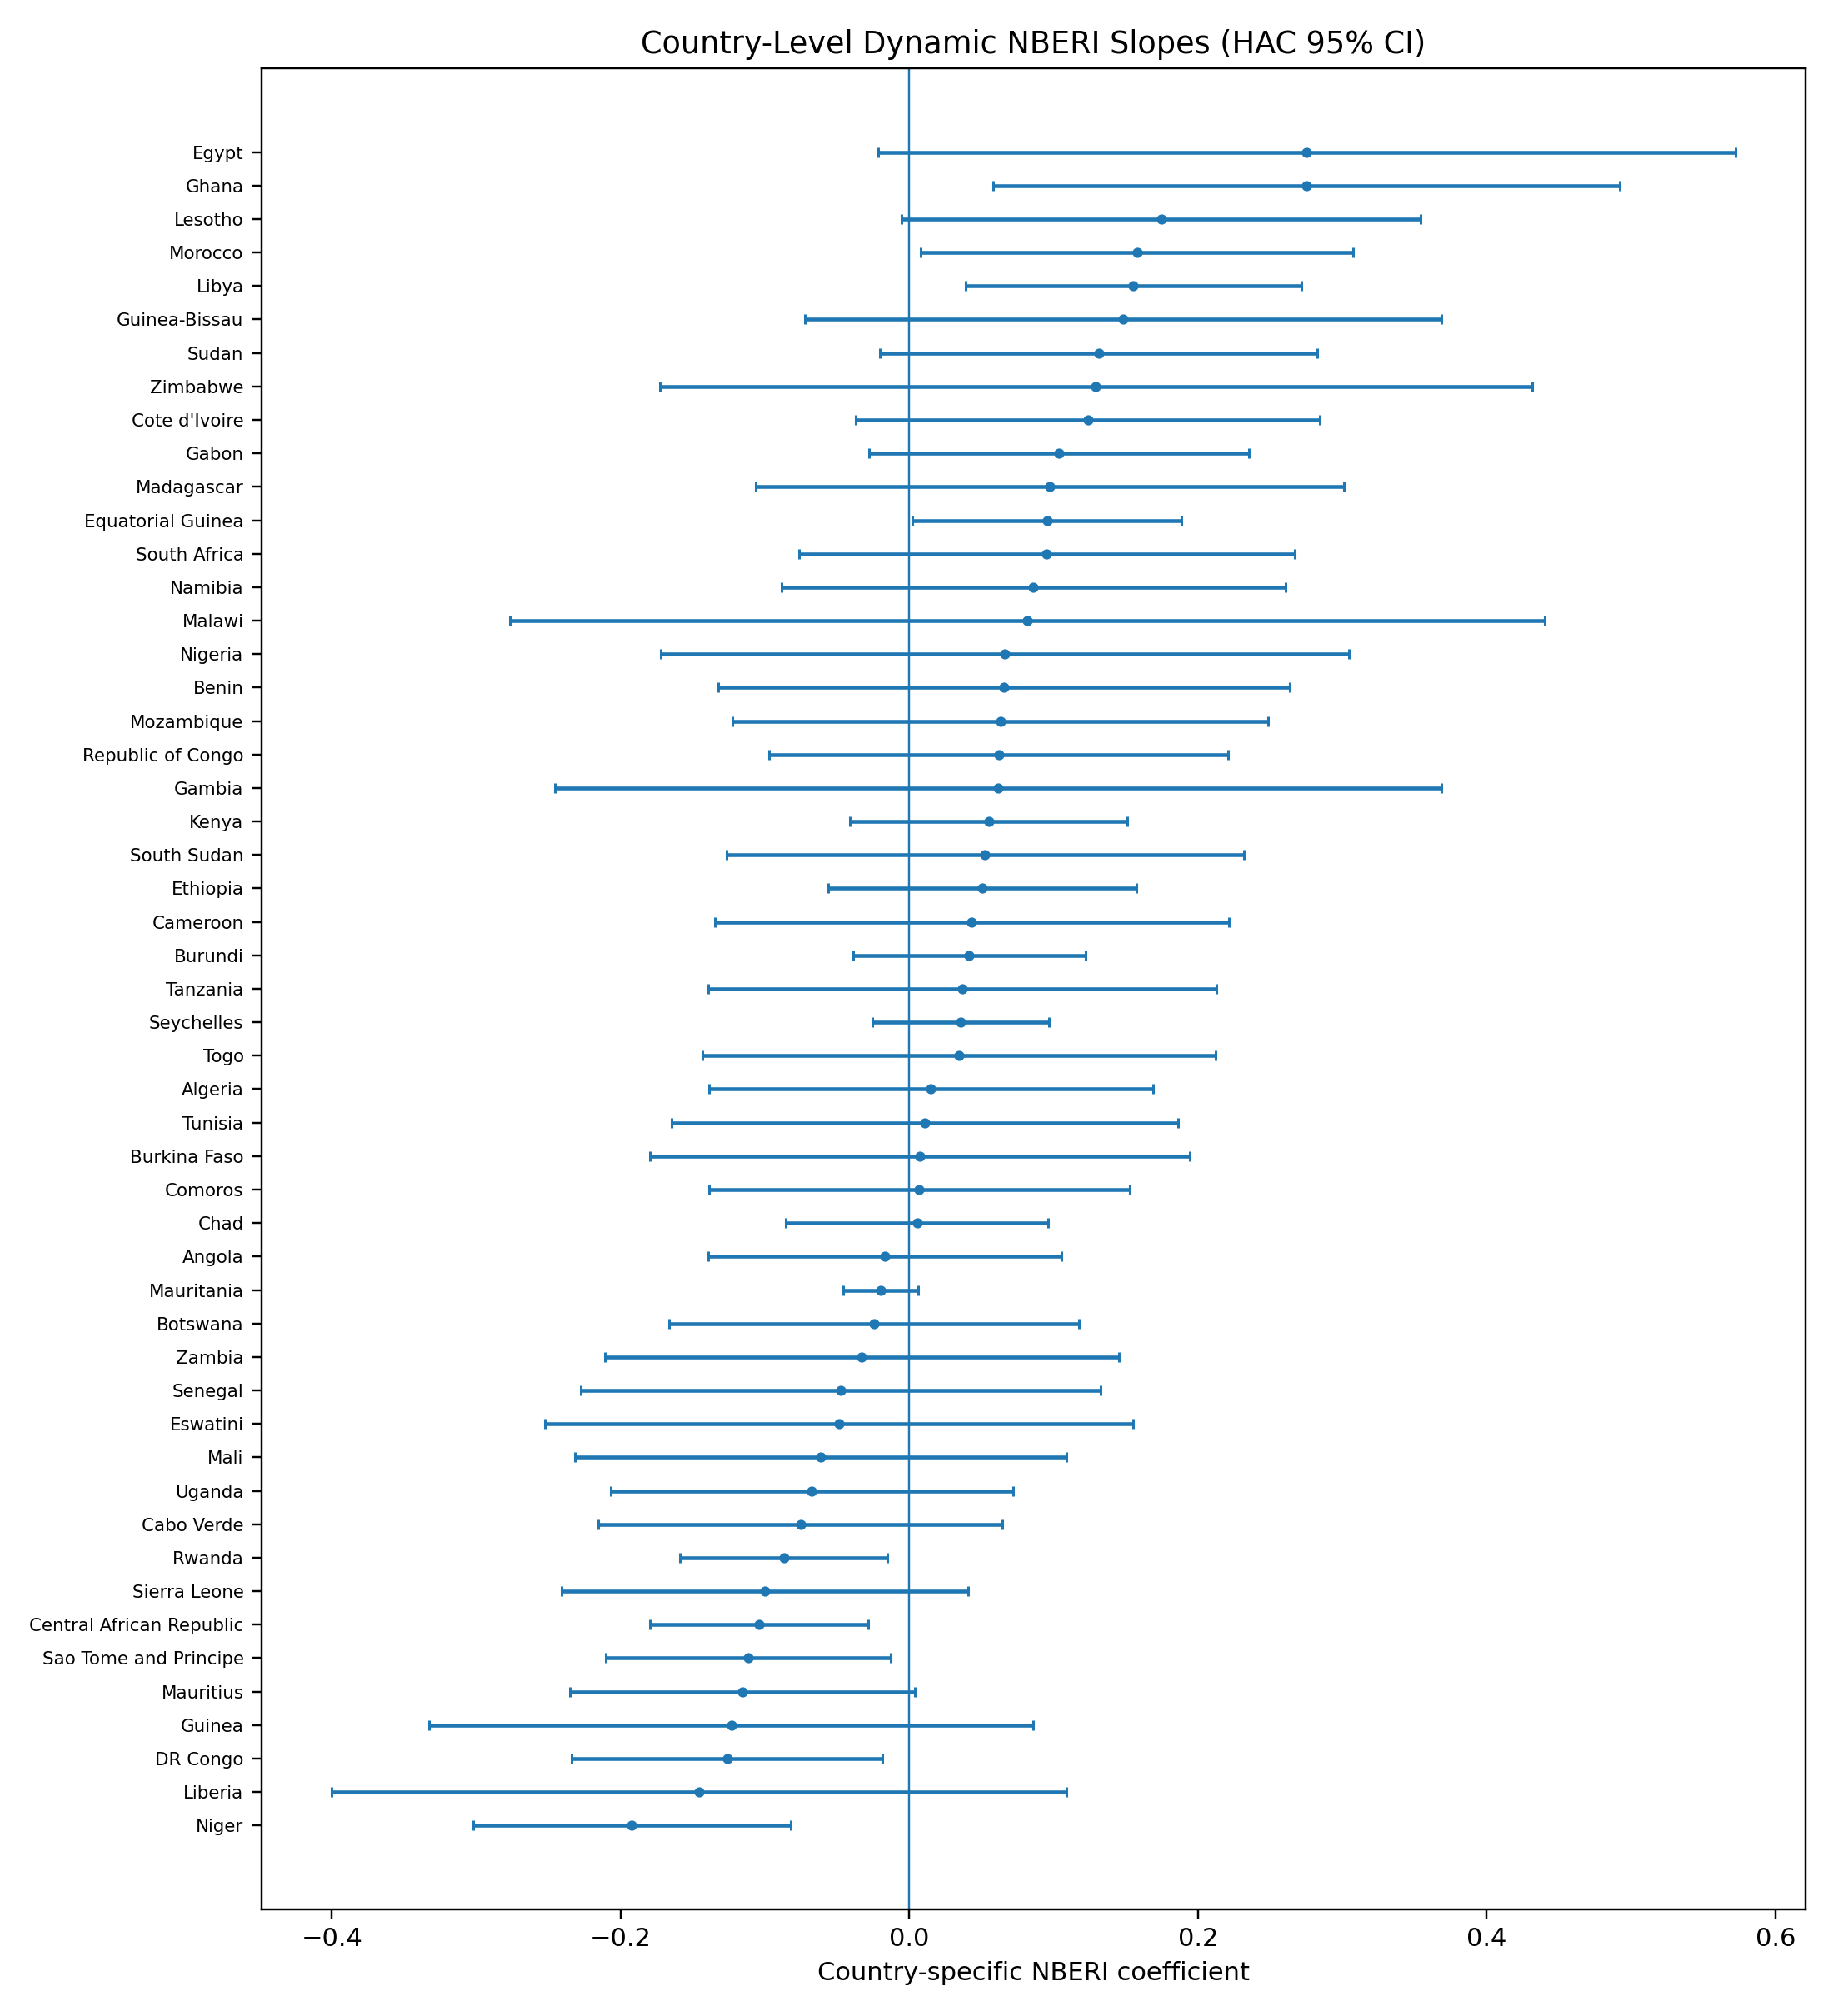
\includegraphics[width=6.3in]{figures/figureD1_country_dynamic_slopes.png}
\caption{Country-level dynamic NBERI slopes with HAC 95 percent confidence intervals.}
\label{fig:13}
\end{figure}

\textbf{Table D1. Country-specific dynamic NBERI slopes}

\begingroup\footnotesize
\begin{longtable}[]{@{}
  >{\raggedright\arraybackslash}p{(\columnwidth - 12\tabcolsep) * \real{0.1429}}
  >{\raggedright\arraybackslash}p{(\columnwidth - 12\tabcolsep) * \real{0.1429}}
  >{\raggedright\arraybackslash}p{(\columnwidth - 12\tabcolsep) * \real{0.1429}}
  >{\raggedright\arraybackslash}p{(\columnwidth - 12\tabcolsep) * \real{0.1429}}
  >{\raggedright\arraybackslash}p{(\columnwidth - 12\tabcolsep) * \real{0.1429}}
  >{\raggedright\arraybackslash}p{(\columnwidth - 12\tabcolsep) * \real{0.1429}}
  >{\raggedright\arraybackslash}p{(\columnwidth - 12\tabcolsep) * \real{0.1429}}@{}}
\toprule\noalign{}
\begin{minipage}[b]{\linewidth}\raggedright
\textbf{Country}
\end{minipage} & \begin{minipage}[b]{\linewidth}\raggedright
\textbf{Region}
\end{minipage} & \begin{minipage}[b]{\linewidth}\raggedright
\textbf{N}
\end{minipage} & \begin{minipage}[b]{\linewidth}\raggedright
\textbf{Beta}
\end{minipage} & \begin{minipage}[b]{\linewidth}\raggedright
\textbf{HAC SE}
\end{minipage} & \begin{minipage}[b]{\linewidth}\raggedright
\textbf{p-value}
\end{minipage} & \begin{minipage}[b]{\linewidth}\raggedright
\textbf{BH q}
\end{minipage} \\
\midrule\noalign{}
\endhead
\bottomrule\noalign{}
\endlastfoot
Angola & Central & 130 & -0.017 & 0.062 & 0.786 & 0.871 \\
Cameroon & Central & 130 & 0.043 & 0.091 & 0.633 & 0.832 \\
Central African Republic & Central & 126 & -0.104 & 0.039 & 0.007 &
0.152 \\
Chad & Central & 130 & 0.006 & 0.046 & 0.905 & 0.937 \\
DR Congo & Central & 114 & -0.126 & 0.055 & 0.022 & 0.183 \\
Equatorial Guinea & Central & 130 & 0.095 & 0.048 & 0.045 & 0.253 \\
Gabon & Central & 130 & 0.104 & 0.067 & 0.122 & 0.430 \\
Republic of Congo & Central & 126 & 0.062 & 0.081 & 0.445 & 0.732 \\
Sao Tome and Principe & Central & 127 & -0.112 & 0.050 & 0.027 &
0.194 \\
Burundi & East & 124 & 0.042 & 0.041 & 0.311 & 0.621 \\
Comoros & East & 129 & 0.007 & 0.074 & 0.924 & 0.937 \\
Ethiopia & East & 127 & 0.051 & 0.055 & 0.353 & 0.621 \\
Kenya & East & 130 & 0.055 & 0.049 & 0.261 & 0.609 \\
Madagascar & East & 129 & 0.097 & 0.104 & 0.349 & 0.621 \\
Mauritius & East & 130 & -0.116 & 0.061 & 0.058 & 0.268 \\
Rwanda & East & 130 & -0.087 & 0.037 & 0.018 & 0.181 \\
Seychelles & East & 130 & 0.036 & 0.031 & 0.256 & 0.609 \\
South Sudan & East & 114 & 0.053 & 0.091 & 0.564 & 0.822 \\
Tanzania & East & 122 & 0.037 & 0.090 & 0.683 & 0.832 \\
Uganda & East & 130 & -0.068 & 0.071 & 0.342 & 0.621 \\
Algeria & North & 130 & 0.015 & 0.079 & 0.848 & 0.921 \\
Egypt & North & 130 & 0.275 & 0.151 & 0.069 & 0.293 \\
Libya & North & 125 & 0.155 & 0.059 & 0.009 & 0.152 \\
Morocco & North & 130 & 0.158 & 0.076 & 0.039 & 0.247 \\
Sudan & North & 96 & 0.131 & 0.077 & 0.089 & 0.351 \\
Tunisia & North & 128 & 0.011 & 0.090 & 0.905 & 0.937 \\
Botswana & Southern & 130 & -0.024 & 0.072 & 0.737 & 0.835 \\
Eswatini & Southern & 130 & -0.049 & 0.104 & 0.640 & 0.832 \\
Lesotho & Southern & 130 & 0.174 & 0.092 & 0.057 & 0.268 \\
Malawi & Southern & 115 & 0.082 & 0.183 & 0.654 & 0.832 \\
Mozambique & Southern & 126 & 0.063 & 0.095 & 0.505 & 0.773 \\
Namibia & Southern & 130 & 0.086 & 0.089 & 0.334 & 0.621 \\
South Africa & Southern & 130 & 0.095 & 0.088 & 0.276 & 0.613 \\
Zambia & Southern & 130 & -0.033 & 0.091 & 0.718 & 0.832 \\
Zimbabwe & Southern & 68 & 0.129 & 0.154 & 0.402 & 0.683 \\
Benin & West & 130 & 0.066 & 0.101 & 0.515 & 0.773 \\
Burkina Faso & West & 130 & 0.008 & 0.095 & 0.937 & 0.937 \\
Cabo Verde & West & 130 & -0.075 & 0.071 & 0.292 & 0.620 \\
Cote d\textquotesingle Ivoire & West & 130 & 0.124 & 0.082 & 0.131 &
0.430 \\
Gambia & West & 130 & 0.062 & 0.157 & 0.694 & 0.832 \\
Ghana & West & 130 & 0.275 & 0.111 & 0.013 & 0.166 \\
Guinea & West & 75 & -0.123 & 0.107 & 0.249 & 0.609 \\
Guinea-Bissau & West & 130 & 0.148 & 0.112 & 0.188 & 0.531 \\
Liberia & West & 126 & -0.145 & 0.130 & 0.263 & 0.609 \\
Mali & West & 129 & -0.061 & 0.087 & 0.480 & 0.764 \\
Mauritania & West & 114 & -0.020 & 0.013 & 0.135 & 0.430 \\
Niger & West & 130 & -0.192 & 0.056 & \textless0.001 & 0.032 \\
Nigeria & West & 130 & 0.066 & 0.122 & 0.587 & 0.832 \\
Senegal & West & 130 & -0.047 & 0.092 & 0.606 & 0.832 \\
Sierra Leone & West & 107 & -0.100 & 0.072 & 0.165 & 0.494 \\
Togo & West & 130 & 0.035 & 0.091 & 0.702 & 0.832 \\
\end{longtable}
\endgroup

\section{Conditional-Variance Robustness}\label{appendix-e.-conditional-variance-robustness}

A pooled GJR-GARCH-X model tests whether a common sign-dependent
innovation response alters the NBERI conclusion. The asymmetry parameter
is effectively zero, and the NBERI coefficient remains statistically
insignificant. This result does not support a common leverage channel in
the monthly panel.

\textbf{Table E1. Pooled GJR-GARCH-X robustness}

\begingroup\footnotesize
\begin{longtable}[]{@{}
  >{\raggedright\arraybackslash}p{(\columnwidth - 12\tabcolsep) * \real{0.1429}}
  >{\raggedright\arraybackslash}p{(\columnwidth - 12\tabcolsep) * \real{0.1429}}
  >{\raggedright\arraybackslash}p{(\columnwidth - 12\tabcolsep) * \real{0.1429}}
  >{\raggedright\arraybackslash}p{(\columnwidth - 12\tabcolsep) * \real{0.1429}}
  >{\raggedright\arraybackslash}p{(\columnwidth - 12\tabcolsep) * \real{0.1429}}
  >{\raggedright\arraybackslash}p{(\columnwidth - 12\tabcolsep) * \real{0.1429}}
  >{\raggedright\arraybackslash}p{(\columnwidth - 12\tabcolsep) * \real{0.1429}}@{}}
\toprule\noalign{}
\begin{minipage}[b]{\linewidth}\raggedright
\textbf{Model}
\end{minipage} & \begin{minipage}[b]{\linewidth}\raggedright
\textbf{Parameter}
\end{minipage} & \begin{minipage}[b]{\linewidth}\raggedright
\textbf{Estimate}
\end{minipage} & \begin{minipage}[b]{\linewidth}\raggedright
\textbf{SE}
\end{minipage} & \begin{minipage}[b]{\linewidth}\raggedright
\textbf{p-value}
\end{minipage} & \begin{minipage}[b]{\linewidth}\raggedright
\textbf{AIC}
\end{minipage} & \begin{minipage}[b]{\linewidth}\raggedright
\textbf{BIC}
\end{minipage} \\
\midrule\noalign{}
\endhead
\bottomrule\noalign{}
\endlastfoot
Panel GJR-GARCH & omega & 0.0289 & & & 14986.9873 & 15020.8434 \\
Panel GJR-GARCH & alpha & 0.3530 & & & 14986.9873 & 15020.8434 \\
Panel GJR-GARCH & gamma\_asymmetry & 0.0000 & & & 14986.9873 &
15020.8434 \\
Panel GJR-GARCH & beta & 0.6420 & & & 14986.9873 & 15020.8434 \\
Panel GJR-GARCH & Student\_t\_df & 4.1409 & & & 14986.9873 &
15020.8434 \\
Panel GJR-GARCH-X & omega & 0.0288 & & & 14988.7966 & 15029.4239 \\
Panel GJR-GARCH-X & alpha & 0.3533 & & & 14988.7966 & 15029.4239 \\
Panel GJR-GARCH-X & gamma\_asymmetry & 0.0000 & & & 14988.7966 &
15029.4239 \\
Panel GJR-GARCH-X & beta & 0.6417 & & & 14988.7966 & 15029.4239 \\
Panel GJR-GARCH-X & delta\_NBERI & -0.0046 & 0.011 & 0.663 & 14988.7966
& 15029.4239 \\
Panel GJR-GARCH-X & Student\_t\_df & 4.1419 & & & 14988.7966 &
15029.4239 \\
\end{longtable}
\endgroup

\section{Reproducibility Definitions}\label{appendix-f.-reproducibility-definitions}

The principal analysis uses the following fixed definitions: (i) monthly
FX return equals 100 times the first log difference of local currency
per U.S. dollar; (ii) the monthly volatility proxy equals \(\ln(1+r^2)\);
(iii) pooled variables are standardized within country; (iv) the
principal dynamic panel uses one lag of NBERI, volatility, return, and
inflation; (v) Driscoll-Kraay bandwidth is four months; (vi) the
shared-currency robustness reduces 51 country series to 36 market
clusters; and (vii) the forecast horse race uses an expanding window
with training-only standardization at every forecast origin. These
definitions are fixed across the reported tables and figures.

\section{Market-Alignment Robustness}\label{appendix-g.-market-alignment-robustness}

The market-alignment ranking is descriptive and is not used as a causal
identifying assumption. Table G1 reports rank-based and detrended
sensitivity measures for the selected countries. Positive raw
correlation is common across the group, but detrended associations vary
materially, which is consistent with using alignment as a heterogeneity
screen rather than a structural parameter.

Table G1. Market-alignment sensitivity diagnostics

\begingroup\footnotesize
\begin{longtable}[]{@{}
  >{\raggedright\arraybackslash}p{(\columnwidth - 8\tabcolsep) * \real{0.2000}}
  >{\raggedright\arraybackslash}p{(\columnwidth - 8\tabcolsep) * \real{0.2000}}
  >{\raggedright\arraybackslash}p{(\columnwidth - 8\tabcolsep) * \real{0.2000}}
  >{\raggedright\arraybackslash}p{(\columnwidth - 8\tabcolsep) * \real{0.2000}}
  >{\raggedright\arraybackslash}p{(\columnwidth - 8\tabcolsep) * \real{0.2000}}@{}}
\toprule\noalign{}
\begin{minipage}[b]{\linewidth}\raggedright
\textbf{Country}
\end{minipage} & \begin{minipage}[b]{\linewidth}\raggedright
\textbf{Raw Pearson}
\end{minipage} & \begin{minipage}[b]{\linewidth}\raggedright
\textbf{Spearman}
\end{minipage} & \begin{minipage}[b]{\linewidth}\raggedright
\textbf{Linear detrended}
\end{minipage} & \begin{minipage}[b]{\linewidth}\raggedright
\textbf{Cubic detrended}
\end{minipage} \\
\midrule\noalign{}
\endhead
\bottomrule\noalign{}
\endlastfoot
Zambia & 0.718 & 0.787 & 0.103 & 0.038 \\
Ghana & 0.668 & 0.514 & 0.406 & 0.021 \\
Malawi & 0.649 & 0.467 & 0.358 & 0.225 \\
Tanzania & 0.561 & 0.641 & -0.072 & 0.002 \\
Algeria & 0.549 & 0.562 & 0.542 & 0.477 \\
Burundi & 0.480 & 0.376 & 0.241 & -0.003 \\
Libya & 0.415 & 0.411 & 0.351 & 0.268 \\
Nigeria & 0.322 & 0.150 & 0.439 & 0.338 \\
Tunisia & 0.296 & 0.336 & 0.223 & 0.140 \\
Morocco & 0.285 & 0.237 & 0.327 & 0.283 \\
Liberia & 0.279 & 0.316 & 0.573 & 0.255 \\
Namibia & 0.268 & 0.287 & 0.434 & 0.443 \\
Congo DRC & 0.266 & 0.343 & 0.319 & 0.258 \\
Guinea & 0.263 & 0.382 & -0.062 & -0.180 \\
Benin & 0.247 & 0.325 & 0.256 & 0.289 \\
\end{longtable}
\endgroup

\section{Full Profile-Likelihood GARCH-Family Results}\label{appendix-h.-full-profile-likelihood-garch-family-results}

Tables H1a-H1c report all 45 country-family X tests after
profile-likelihood refinement. BH q-values are computed separately
within GARCH-X, EGARCH-X, and GJR/TGARCH-X across the 15 countries.

Table H1a. GARCH-X country results

\begingroup\footnotesize
\begin{longtable}[]{@{}
  >{\raggedright\arraybackslash}p{(\columnwidth - 14\tabcolsep) * \real{0.1250}}
  >{\raggedright\arraybackslash}p{(\columnwidth - 14\tabcolsep) * \real{0.1250}}
  >{\raggedright\arraybackslash}p{(\columnwidth - 14\tabcolsep) * \real{0.1250}}
  >{\raggedright\arraybackslash}p{(\columnwidth - 14\tabcolsep) * \real{0.1250}}
  >{\raggedright\arraybackslash}p{(\columnwidth - 14\tabcolsep) * \real{0.1250}}
  >{\raggedright\arraybackslash}p{(\columnwidth - 14\tabcolsep) * \real{0.1250}}
  >{\raggedright\arraybackslash}p{(\columnwidth - 14\tabcolsep) * \real{0.1250}}
  >{\raggedright\arraybackslash}p{(\columnwidth - 14\tabcolsep) * \real{0.1250}}@{}}
\toprule\noalign{}
\begin{minipage}[b]{\linewidth}\raggedright
\textbf{Country}
\end{minipage} & \begin{minipage}[b]{\linewidth}\raggedright
\textbf{delta}
\end{minipage} & \begin{minipage}[b]{\linewidth}\raggedright
\textbf{LR p}
\end{minipage} & \begin{minipage}[b]{\linewidth}\raggedright
\textbf{BH q}
\end{minipage} & \begin{minipage}[b]{\linewidth}\raggedright
\textbf{AIC}
\end{minipage} & \begin{minipage}[b]{\linewidth}\raggedright
\textbf{LB sq. p}
\end{minipage} & \begin{minipage}[b]{\linewidth}\raggedright
\textbf{ARCH-LM p}
\end{minipage} & \begin{minipage}[b]{\linewidth}\raggedright
\textbf{Profile grid}
\end{minipage} \\
\midrule\noalign{}
\endhead
\bottomrule\noalign{}
\endlastfoot
Algeria & 0.161 & 0.4252 & 1.0000 & 311.1 & 0.976 & 0.980 & 0.15 \\
Benin & 0.149 & 0.4531 & 1.0000 & 502.2 & 0.240 & 0.272 & 0.15 \\
Burundi & 0.000 & 1.0000 & 1.0000 & -346.0 & 1.000 & 1.000 & -0.50 \\
Congo DRC & 0.000 & 1.0000 & 1.0000 & 285.4 & 0.967 & 0.975 & 0.75 \\
Ghana & 0.000 & 1.0000 & 1.0000 & 624.9 & 0.017 & 0.024 & 1.00 \\
Guinea & 0.000 & 1.0000 & 1.0000 & 142.5 & 0.471 & 0.422 & 0.00 \\
Liberia & 0.000 & 1.0000 & 1.0000 & 500.0 & 0.886 & 0.899 & 0.50 \\
Libya & 0.645 & 0.0005 & 0.0074 & 375.9 & 1.000 & 1.000 & 0.75 \\
Malawi & 0.000 & 1.0000 & 1.0000 & 278.1 & 1.000 & 1.000 & 0.50 \\
Morocco & 0.000 & 1.0000 & 1.0000 & 433.3 & 0.786 & 0.732 & 0.15 \\
Namibia & 0.214 & 0.1639 & 1.0000 & 686.2 & 0.983 & 0.986 & 0.15 \\
Nigeria & 0.000 & 1.0000 & 1.0000 & 440.3 & 0.997 & 0.997 & 0.30 \\
Tanzania & 0.127 & 0.2634 & 1.0000 & -4.6 & 0.998 & 0.999 & 0.15 \\
Tunisia & -0.031 & 0.7384 & 1.0000 & 453.3 & 0.841 & 0.856 & 0.00 \\
Zambia & -0.036 & 0.7422 & 1.0000 & 748.8 & 0.954 & 0.945 & 0.00 \\
\end{longtable}
\endgroup

Table H1b. EGARCH-X country results

\begingroup\footnotesize
\begin{longtable}[]{@{}
  >{\raggedright\arraybackslash}p{(\columnwidth - 14\tabcolsep) * \real{0.1250}}
  >{\raggedright\arraybackslash}p{(\columnwidth - 14\tabcolsep) * \real{0.1250}}
  >{\raggedright\arraybackslash}p{(\columnwidth - 14\tabcolsep) * \real{0.1250}}
  >{\raggedright\arraybackslash}p{(\columnwidth - 14\tabcolsep) * \real{0.1250}}
  >{\raggedright\arraybackslash}p{(\columnwidth - 14\tabcolsep) * \real{0.1250}}
  >{\raggedright\arraybackslash}p{(\columnwidth - 14\tabcolsep) * \real{0.1250}}
  >{\raggedright\arraybackslash}p{(\columnwidth - 14\tabcolsep) * \real{0.1250}}
  >{\raggedright\arraybackslash}p{(\columnwidth - 14\tabcolsep) * \real{0.1250}}@{}}
\toprule\noalign{}
\begin{minipage}[b]{\linewidth}\raggedright
\textbf{Country}
\end{minipage} & \begin{minipage}[b]{\linewidth}\raggedright
\textbf{delta}
\end{minipage} & \begin{minipage}[b]{\linewidth}\raggedright
\textbf{LR p}
\end{minipage} & \begin{minipage}[b]{\linewidth}\raggedright
\textbf{BH q}
\end{minipage} & \begin{minipage}[b]{\linewidth}\raggedright
\textbf{AIC}
\end{minipage} & \begin{minipage}[b]{\linewidth}\raggedright
\textbf{LB sq. p}
\end{minipage} & \begin{minipage}[b]{\linewidth}\raggedright
\textbf{ARCH-LM p}
\end{minipage} & \begin{minipage}[b]{\linewidth}\raggedright
\textbf{Profile grid}
\end{minipage} \\
\midrule\noalign{}
\endhead
\bottomrule\noalign{}
\endlastfoot
Algeria & 0.000 & 1.0000 & 1.0000 & 325.3 & 0.968 & 0.970 & 0.00 \\
Benin & 0.000 & 1.0000 & 1.0000 & 502.3 & 0.382 & 0.337 & 0.00 \\
Burundi & 0.000 & 1.0000 & 1.0000 & -138.5 & 1.000 & 1.000 & 1.00 \\
Congo DRC & 0.000 & 1.0000 & 1.0000 & 223.5 & 0.983 & 0.979 & -0.30 \\
Ghana & 0.766 & 0.0002 & 0.0036 & 574.0 & 0.044 & 0.078 & 1.00 \\
Guinea & 0.154 & 0.5751 & 1.0000 & 124.5 & 0.856 & 0.737 & 0.15 \\
Liberia & -0.068 & 0.4264 & 1.0000 & 466.7 & 0.943 & 0.930 & 0.00 \\
Libya & 0.000 & 1.0000 & 1.0000 & 467.6 & 1.000 & 1.000 & 0.75 \\
Malawi & 0.000 & 1.0000 & 1.0000 & 519.0 & 0.999 & 0.999 & 1.00 \\
Morocco & 0.000 & 1.0000 & 1.0000 & 436.1 & 0.301 & 0.167 & 0.15 \\
Namibia & 0.000 & 1.0000 & 1.0000 & 685.7 & 0.454 & 0.568 & 0.00 \\
Nigeria & 0.000 & 1.0000 & 1.0000 & 731.2 & 0.998 & 0.998 & 1.00 \\
Tanzania & 0.000 & 1.0000 & 1.0000 & 218.9 & 0.458 & 0.013 & 0.30 \\
Tunisia & -0.042 & 0.3696 & 1.0000 & 454.2 & 0.765 & 0.793 & 0.00 \\
Zambia & 0.000 & 1.0000 & 1.0000 & 767.6 & 0.992 & 0.993 & 0.00 \\
\end{longtable}
\endgroup

Table H1c. GJR/TGARCH-X country results

\begingroup\footnotesize
\begin{longtable}[]{@{}
  >{\raggedright\arraybackslash}p{(\columnwidth - 14\tabcolsep) * \real{0.1250}}
  >{\raggedright\arraybackslash}p{(\columnwidth - 14\tabcolsep) * \real{0.1250}}
  >{\raggedright\arraybackslash}p{(\columnwidth - 14\tabcolsep) * \real{0.1250}}
  >{\raggedright\arraybackslash}p{(\columnwidth - 14\tabcolsep) * \real{0.1250}}
  >{\raggedright\arraybackslash}p{(\columnwidth - 14\tabcolsep) * \real{0.1250}}
  >{\raggedright\arraybackslash}p{(\columnwidth - 14\tabcolsep) * \real{0.1250}}
  >{\raggedright\arraybackslash}p{(\columnwidth - 14\tabcolsep) * \real{0.1250}}
  >{\raggedright\arraybackslash}p{(\columnwidth - 14\tabcolsep) * \real{0.1250}}@{}}
\toprule\noalign{}
\begin{minipage}[b]{\linewidth}\raggedright
\textbf{Country}
\end{minipage} & \begin{minipage}[b]{\linewidth}\raggedright
\textbf{delta}
\end{minipage} & \begin{minipage}[b]{\linewidth}\raggedright
\textbf{LR p}
\end{minipage} & \begin{minipage}[b]{\linewidth}\raggedright
\textbf{BH q}
\end{minipage} & \begin{minipage}[b]{\linewidth}\raggedright
\textbf{AIC}
\end{minipage} & \begin{minipage}[b]{\linewidth}\raggedright
\textbf{LB sq. p}
\end{minipage} & \begin{minipage}[b]{\linewidth}\raggedright
\textbf{ARCH-LM p}
\end{minipage} & \begin{minipage}[b]{\linewidth}\raggedright
\textbf{Profile grid}
\end{minipage} \\
\midrule\noalign{}
\endhead
\bottomrule\noalign{}
\endlastfoot
Algeria & 0.000 & 1.0000 & 1.0000 & 337.8 & 0.989 & 0.990 & 0.00 \\
Benin & 0.000 & 1.0000 & 1.0000 & 505.7 & 0.127 & 0.155 & 0.00 \\
Burundi & 0.000 & 1.0000 & 1.0000 & 335.9 & 1.000 & 1.000 & 0.00 \\
Congo DRC & 0.000 & 1.0000 & 1.0000 & 429.4 & 0.956 & 0.957 & 0.00 \\
Ghana & 0.000 & 1.0000 & 1.0000 & 695.2 & 0.775 & 0.721 & 0.75 \\
Guinea & 0.000 & 1.0000 & 1.0000 & 143.7 & 0.484 & 0.417 & 0.30 \\
Liberia & 0.000 & 1.0000 & 1.0000 & 502.4 & 0.868 & 0.874 & 0.00 \\
Libya & 0.000 & 1.0000 & 1.0000 & 745.5 & 1.000 & 1.000 & 0.00 \\
Malawi & 0.000 & 1.0000 & 1.0000 & 516.8 & 0.999 & 0.999 & -0.15 \\
Morocco & 0.000 & 1.0000 & 1.0000 & 440.3 & 0.180 & 0.061 & 0.30 \\
Namibia & 0.000 & 1.0000 & 1.0000 & 689.7 & 0.543 & 0.640 & 0.00 \\
Nigeria & 0.000 & 1.0000 & 1.0000 & 726.4 & 0.998 & 0.998 & 1.00 \\
Tanzania & 0.000 & 1.0000 & 1.0000 & 51.4 & 0.977 & 0.880 & 0.15 \\
Tunisia & 0.000 & 1.0000 & 1.0000 & 460.8 & 0.802 & 0.836 & 0.00 \\
Zambia & 0.000 & 1.0000 & 1.0000 & 771.1 & 0.966 & 0.958 & 0.30 \\
\end{longtable}
\endgroup

\section{Random-Subset Benchmark}\label{appendix-i.-random-subset-benchmark}

To assess whether the selected-15 fixed-effects slope is unusually large
relative to arbitrary country groupings, 1,000 subsets of 15 countries
are drawn without replacement from the 51 eligible markets. The selected
group\textquotesingle s incremental slope is at the 94.1st percentile of
the random distribution and its total slope is at the 94.4th percentile.
The corresponding one-sided empirical probabilities are 0.060 and 0.057.
These values are suggestive rather than conventionally significant and
are interpreted accordingly.

Table I1. Random 15-country subset benchmark

\begingroup\footnotesize
\begin{longtable}[]{@{}
  >{\raggedright\arraybackslash}p{(\columnwidth - 10\tabcolsep) * \real{0.1667}}
  >{\raggedright\arraybackslash}p{(\columnwidth - 10\tabcolsep) * \real{0.1667}}
  >{\raggedright\arraybackslash}p{(\columnwidth - 10\tabcolsep) * \real{0.1667}}
  >{\raggedright\arraybackslash}p{(\columnwidth - 10\tabcolsep) * \real{0.1667}}
  >{\raggedright\arraybackslash}p{(\columnwidth - 10\tabcolsep) * \real{0.1667}}
  >{\raggedright\arraybackslash}p{(\columnwidth - 10\tabcolsep) * \real{0.1667}}@{}}
\toprule\noalign{}
\begin{minipage}[b]{\linewidth}\raggedright
\textbf{Statistic}
\end{minipage} & \begin{minipage}[b]{\linewidth}\raggedright
\textbf{Observed}
\end{minipage} & \begin{minipage}[b]{\linewidth}\raggedright
\textbf{Random mean}
\end{minipage} & \begin{minipage}[b]{\linewidth}\raggedright
\textbf{Random SD}
\end{minipage} & \begin{minipage}[b]{\linewidth}\raggedright
\textbf{Percentile}
\end{minipage} & \begin{minipage}[b]{\linewidth}\raggedright
\textbf{Empirical p}
\end{minipage} \\
\midrule\noalign{}
\endhead
\bottomrule\noalign{}
\endlastfoot
Selected-15 incremental slope & 0.044 & -0.001 & 0.030 & 94.1 & 0.060 \\
Selected-15 total slope & 0.061 & 0.028 & 0.021 & 94.4 & 0.057 \\
\end{longtable}
\endgroup


\end{document}
